\RequirePackage[ngerman=ngerman-x-latest]{hyphsubst}
\documentclass[english,ngerman]{tudscrreprt}
\usepackage{babel}
\usepackage{selinput}
\SelectInputMappings{adieresis={ä},germandbls={ß}}
\usepackage[T1]{fontenc}
\usepackage{fixltx2e}
\usepackage{scrhack}
\usepackage{tudscrsupervisor}
\usepackage{xcolor}
\usepackage{gensymb}

%%%
% Glossar
%
\AfterPackage*{hyperref}{%
	\usepackage[%
		automake,% Alphabetische Sortierung, da xindy aktiv, kein makeindex benötigt
		% mit Tex Live einfach verwendbar
		xindy={language=german-din}, % Alphabetische Sortierung nach UTF-8 und Duden oder DIN.
		acronym,% Abkürzungen
		symbols,% Formelzeichen
		%nomain,% kein Glossar
		translate=babel,% Überschriften der Glossare in der Dokumentsprache gesetzt
		nogroupskip,% automatischer Abstand zwischen den Einträgen zur Gruppierung innerhalb eines Glossars entfernen
		toc,% fügt die Verzeichnisse dem Inhaltsverzeichnis hinzu
		section=chapter,% bestimmt die Gliederungsebene der Überschrift
	]{glossaries}
	\makeglossaries
	
\newglossarystyle{acrotabu}{%
	\renewenvironment{theglossary}{%
		\begin{tabu}spread 0pt{@{}lX<{\strut}l@{}}%
	}{%
		\end{tabu}\par\bigskip%
	}%
	\renewcommand*{\glossaryheader}{}%
	\renewcommand*{\glsgroupheading}[1]{}%
	\renewcommand*{\glsgroupskip}{}%
	\renewcommand*{\glossentry}[2]{%
		\glsentryitem{##1}% Entry number if required
		\glstarget{##1}{\sffamily\bfseries\glossentryname{##1}} &
		\glsentrydesc{##1} &
		##2\tabularnewline
	}
}

\newcommand*{\newsymbol}[5][]{%
	\newglossaryentry{#2}{%
		type=symbols,%
		description={},%
		name={#3},%
		symbol={\ensuremath{#4}},%
		user1={\ensuremath{\mathrm{#5}}},%
		sort={#2},%
		#1%
	}%
}

\defglsentryfmt[symbols]{%
	\ifmmode%
	\glssymbol{\glslabel}%
	\else%
	\glsgenentryfmt~\glsentrysymbol{\glslabel}%
	\fi%
}
\newglossarystyle{symblongtabu}{%
	\renewenvironment{theglossary}{%
		\begin{longtabu}spread 0pt[l]{ccX<{\strut}l}%
		}{%
		\end{longtabu}%
	}%
	\renewcommand*{\glossaryheader}{%
		\toprule
		\bfseries Symbol & \bfseries Einheit &
		\bfseries Name & \bfseries Seite(n)
		\tabularnewline\midrule\endhead%
		\bottomrule\endfoot%
	}%
	\renewcommand*{\glsgroupheading}[1]{}%
	\renewcommand*{\glsgroupskip}{}%
	\renewcommand*{\glossentry}[2]{%
		\glsentryitem{##1}% Entry number if required
		\glstarget{##1}{\glossentrysymbol{##1}} &
		\glsentryuseri{##1} &
		\glossentryname{##1} &
		##2\tabularnewline%
	}%
}
}% Ende von AfterPackage*

%%%
% Zitate
%
\usepackage{csquotes}
\usepackage[backend=biber,style=alphabetic]{biblatex}
\addbibresource{bib/MMandCountourTrees.bib}
\addbibresource{bib/Polyeder.bib}

%%%
% Caption
%
\usepackage{caption}
\captionsetup{font=sf,labelfont=bf,labelsep=space}
\usepackage{floatrow}
\floatsetup{font=sf}
\floatsetup[table]{style=plaintop}
\captionsetup{singlelinecheck=off,format=hang,justification=raggedright}
\DeclareCaptionSubType[alph]{figure}
\DeclareCaptionSubType[alph]{table}
\captionsetup[subfloat]{labelformat=brace,list=off}

%%%
% Tabellen
%
\usepackage{booktabs} % Linien für Tabellen.
\usepackage{array} % Definitionen für Spalten.
\usepackage{tabularx} % Tabellen mit gleicher Spaltenbreite.
\usepackage{tabulary}
\usepackage{tabu}


%%%
% Index
%
\usepackage{imakeidx}
\indexsetup{%
	level=\chapter*,
	noclearpage, firstpagestyle=headings, headers={\indexname}{\indexname},
	othercode={\renewcommand*\subitem{\@idxitem\hspace*{15\p@}}}
}\makeindex

%%%
% Bilder
%
\usepackage{graphicx}
\graphicspath{ {./media/} }

%%%
% Quellcode
%
\usepackage{listings}
% UTF8
\lstset{%
	inputencoding = utf8,
	extendedchars = true, % lets you use non-ASCII characters; for 8-bits encodings only, does not work with UTF-8
	literate=%
	{ä}{{\"a}}1 {ö}{{\"o}}1 {ü}{{\"u}}1
	{Ä}{{\"A}}1 {Ö}{{\"O}}1 {Ü}{{\"U}}1
	{~}{{\textasciitilde}}1 {ß}{{\ss}}1
}
\definecolor{dkgreen}{rgb}{0,0.6,0}
\definecolor{mygray}{rgb}{0.5,0.5,0.5}
\definecolor{mymauve}{rgb}{0.58,0,0.82}
\lstset{ %
	backgroundcolor=\color{white},   % choose the background color; you must add \usepackage{color} or \usepackage{xcolor}
	basicstyle=\footnotesize,        % the size of the fonts that are used for the code
	breakatwhitespace=false,         % sets if automatic breaks should only happen at whitespace
	breaklines=true,                 % sets automatic line breaking
	captionpos=b,                    % sets the caption-position to bottom
	commentstyle=\color{dkgreen},    % comment style
	deletekeywords={...},            % if you want to delete keywords from the given language
	escapeinside={\%*}{*)},          % if you want to add LaTeX within your code
	frame=single,                    % adds a frame around the code
	keepspaces=true,                 % keeps spaces in text, useful for keeping indentation of code (possibly needs columns=flexible)
	keywordstyle=\color{blue},       % keyword style
	language=Octave,                 % the language of the code
	morekeywords={*,...},            % if you want to add more keywords to the set
	numbers=left,                    % where to put the line-numbers; possible values are (none, left, right)
	numbersep=5pt,                   % how far the line-numbers are from the code
	numberstyle=\tiny\color{mygray}, % the style that is used for the line-numbers
	rulecolor=\color{black},         % if not set, the frame-color may be changed on line-breaks within not-black text (e.g. comments (green here))
	showspaces=false,                % show spaces everywhere adding particular underscores; it overrides 'showstringspaces'
	showstringspaces=false,          % underline spaces within strings only
	showtabs=false,                  % show tabs within strings adding particular underscores
	stepnumber=2,                    % the step between two line-numbers. If it's 1, each line will be numbered
	stringstyle=\color{mymauve},     % string literal style
	tabsize=2,                       % sets default tabsize to 2 spaces
	title=\lstname                   % show the filename of files included with \lstinputlisting; also try caption instead of title
}

%%%
% Links
%
\usepackage{hyperref} % Möglichst am Ende stehen, da es viele Befehle neu definiert.
\hypersetup{
	colorlinks   = true, %Colours links instead of ugly boxes
	urlcolor     = HKS41!70, %Colour for external hyperlinks
	linkcolor    = HKS44!70, %Colour of internal links
	citecolor    = HKS33!80 %Colour of citations
}

\usepackage{quoting}

\usepackage[babel]{microtype}

\usepackage{xfrac}

%%%
% Aufzählungen
%
\usepackage{enumitem}
\setlist[itemize]{noitemsep}
\setlist[description]{noitemsep}

\usepackage{isodate}

\usepackage{ellipsis}
\let\ellipsispunctuation\relax

\usepackage{amssymb} % Muss nach hyperref kommen, sonst Fehler "\newsymbol already defined". Alternative: http://tex.stackexchange.com/questions/73684/are-there-any-situtations-where-it-is-better-to-load-a-package-after-other-code

\usepackage{tikz}
\usetikzlibrary{arrows,positioning,scopes,trees}
%%%
% Index
%
\newcommand{\CFD}{\gls{cfd}\index{CFD-Algorithmus}}
\newcommand{\SECC}{\gls{secc}\index{SECC-Algorithmus}}

%Allgemein
\newcommand{\tool}[1]{\textit{#1}\index{#1}} %und libs. Wg vieler Abkürzungen evtl ins Glossar! (z.B. ANN, OpenMP, PPL)
\newcommand{\tools}[2]{\textit{#1}\index{#2}}
\newcommand{\propername}[1]{\textit{#1}\index{#1}} % Allgemein.
\newcommand{\propernames}[2]{\textit{#1}\index{#2}} % Allgemein.
\newcommand{\SEPlugin}[1]{\textit{#1}\index{#1}} % Programmaufbau, evtl in Glossar umwandeln!
\newcommand{\SEPlugins}[2]{\textit{#1}\index{#2}} % Programmaufbau.

%Visualisierung
\newcommand{\visattr}[1]{\textit{#1}\index{#1}}
\newcommand{\visattrs}[2]{\textit{#1}\index{#2}}
\newcommand{\vis}[1]{\textit{#1}\index{#1}} %Visuelles
\newcommand{\viss}[2]{\textit{#1}\index{#2}} %Visuelles
\newcommand{\dataparam}[1]{\textit{#1}\index{#1}}
\newcommand{\dataparams}[2]{\textit{#1}\index{#2}}

% Berechnung
\newcommand{\contour}[1]{\textit{#1}\index{#1}}
\newcommand{\contours}[2]{\textit{#1}\index{#2}}
\newcommand{\SECterm}[1]{\textit{#1}\index{#1}}
\newcommand{\SECterms}[2]{\textit{#1}\index{#2}}
\newcommand{\CFDterm}[1]{\textit{#1}\index{#1}}
\newcommand{\CFDterms}[2]{\textit{#1}\index{#2}}

%%%
% Auszeichnungen
%
\newcommand{\wichtig}[1]{\textit{#1}}
\newcommand{\mrkg}[1]{\textcolor{orange}{#1}} % Markierung, etwa in Gleichungen
\newcommand{\mrkgb}[1]{\textcolor{magenta}{#1}} % Markierung, etwa in Gleichungen
\newcommand{\libNoIndex}[1]{\textit{#1}}

%%%
% Tabelle
%
\newcolumntype{F}{>{\hspace{0pt}}X}
\newcolumntype{L}{>{\raggedright}F}
\newcolumntype{C}{>{\centering}F}
\newcolumntype{D}{>{\centering}F}
\newcolumntype{R}{>{\raggedleft}F}

%%%
% Symbole
%
\newcommand{\kreuz}{ $\times$ }
\newcommand{\esfolgt}{ $\to$ }
\newcommand{\eqtxt}[1]{\stackrel{\text{#1}}{=}} %Gleichheitszeichen mit Text drüber
\newcommand{\intxt}[1]{\stackrel{\text{#1}}{\in}} %Element von mit Text drüber
\newcommand{\abs}[1]{\lvert#1\rvert}
\newcommand{\norm}[1]{\lVert#1\rVert}
\newcommand{\qed}{$_\square$} %Was zu beweisen war; quod erat demonstrandum

%%%
% TikZ
%
\tikzset {
	value/.style={rectangle, draw},
	vocab/.style={rectangle, draw, rounded corners=.8ex},
	verticalChild/.style={grow=down, xshift=.5em, anchor=west, font = \small,
					edge from parent path={(\tikzparentnode.south) |- (\tikzchildnode.west)}},
	first/.style={level distance=6ex},
	second/.style={level distance=12ex},
	third/.style={level distance=18ex},
	fourth/.style={level distance=24ex},
	level 1/.style={sibling distance=3cm}
}
\newglossaryentry{platonischer Körper}{
	name = {platonischer Körper},
	description = {fünf},
	plural = {platonische Körper},
	sort = {Körper}
}

\newglossaryentry{3dRaum} {
	name = {\ensuremath{\mathbb{R}^3}},
	description = {Dreidimensionaler Raum},
	sort = {R}
}

\newacronym[
	longplural={Relationale Datenbankmanagementsysteme}
	description={Relationales Datenbankmanagementsystem}
]{rdbms}{RDBMS}{Relationalen Datenbankmanagementsystems}

\newacronym[
	longplural={Hue-Saturation-Brightness}
	description={Ein Farbschema mit drei Dimensionen für Farbwert (0°-360°), Sättigung und Helligkeit.}
]{hsb}{HSB}{Hue-Saturation-Brightness}



\newacronym[
	longplural={Pixel}
	description={Eine Einheit.}
]{px}{px}{Pixel}



\newacronym[
longplural={MegaMol Structure Events}
description={Das Dateiformat für die Structure Events.}
]{mmse}{MMSE}{MegaMol Structure Event}

\newacronym[
longplural={Structure Events Cluster Compare}
description={Vergleich von Clustern über zwei Frames.}
]{secc}{SECC}{Structure Events Cluster Compare}

\newacronym[
longplural={Structure Events Data Call}
description={Der MegaMol Call, der zum Übertragen von Structure Events Daten genutzt wird.}
]{sedc}{SEDC}{Structure Events Data Call}

%\usepackage{tudscrman}

\begin{document}

\faculty{Fakultät für Informatik}
%\department{Institut für Software- und Multimediatechnik}
\institute{Institut für Software- und Multimediatechnik}
\chair{Professur Computergraphik und Visualisierung}

\subject{Bachelorarbeit}
%\subject{bachelor}
\title{Visualisierung von Strukturveränderungen in Molekulardynamikdaten}
%Zweittitel: Ritterspiele im Bällebad (Glyphen/blaues Kreuz (Death) in bunten Kugeln) - props to Caro
\thesis{Bachelor}
%\thesis{bachelor}

\graduation[B.Sc.]{Bachelor of Science}
\author{%
	Richard Hähne
	\matriculationnumber{2873574}
	\dateofbirth{10.2.1982}
	\placeofbirth{Dresden}
	\matriculationyear{2011}
	\course{Medieninformatik}
	%\discipline{Informationsvisualisierung}
}

%\referee{Dr. Grottel}
\supervisor{Sebastian Grottel \and Ludwig Schmutzler}
\professor{Prof. Dr. Stefan Gumhold}
\date{2015-08-10}
%\defensedate{2945-12-31}

%\frontmatter %Vorspann: Römische Seitennummerierung

%\makecover
\maketitle

\confirmation \tableofcontents %\listoffigures \listoftables

%\printglossaries %uncomment for using makeglossaries.exe
%\printglossary
\printacronyms[style=acrotabu] \printsymbols[style=symblongtabu]

%\mainmatter %Hauptteil: Normale Seitennummerierung

\chapter{Aufgabenstellung}

Die visuelle Analyse spielt für komplexe, partikelbasierte Daten, wie sie beispielsweise in der Molekulardynamik entstehen, eine immer wichtiger werdende Rolle. Da die Datensätze immer größer werden, gewinnen abstrahierte Visualisierungen zur Vermittlung eines Überblicks zunehmend an Bedeutung. Kritisch ist hierbei vor allem die Darstellung zeitlicher Entwicklungen. Üblicherweise werden diese als Animation oder in rein abstrakter Form dargestellt. Diese Visualisierungen bieten nur einen schlechten zeitlichen Überblick oder stellen kaum Bezug zum ursprünglich simulierten Ortsraum dar.

Ziel dieser Arbeit ist es daher an einem konkreten Beispiel eine Visualisierung zu entwickeln, die im geometrischen Kontext der Originaldaten die zeitliche Entwicklung der Struktur des Datensatzes darstellt. Der zu untersuchende Datensatz (exp2mill.mmpld, 2 Mio. Partikel, 150 Zeitschritte) zeigt einen Flüssigkeitsfilm im Vakuum, der aufgrund seines übergroßen Innendrucks explodiert. Hierbei bilden sich Molekülcluster, -Tröpfchen und –Filamentstrukturen, welche sich über die Zeit hinweg verändern (aufspalten und verschmelzen).

Zunächst soll der Datensatz in mehreren Stufen analysiert werden. Ein erster Schritt bestimmt die Interface-Grenzen zwischen der flüssigen Phase und dem Vakuum, bzw. in späteren Zeitschritten der Gasphase. In einem zweiten Schritt wird auf dieser Basis eine vorzeichenbehaftete Distanzfunktion aufgestellt, die für alle Partikel die Entfernung zum Rand bestimmt. Für diese beiden Arbeitsschritte kann auf bestehenden Quellcode zurückgegriffen werden. Anschließend wird, auf Basis eines vom Benutzer vorgegebenen Schwellwerts die Struktur der Daten, in Form von Clustern/Knoten und Verbindungen, vergleichbar zu einem Contour-Tree extrahiert. Besondere zeitliche Ereignisse sind gekennzeichnet durch Änderungen in dieser Struktur (Split, Merge, Birth, Death). Diese Ereignisse werden, beispielsweise über Glyphen, in einer zeitunabhängigen Ansicht in Ortsraumkoordinaten des Originaldatensatzes visualisiert.

Die entstandene Lösung soll in zweierlei Hinsicht evaluiert werden. Zum einen betrifft dies die Berechnungsgeschwindigkeit. Hierbei ist jedoch eine umfassende Optimierung nicht so wichtig wie die grundsätzliche Komplexität und Skalierbarkeit der eingesetzten Algorithmen. Als zweites soll die entstandene Visualisierung in einer informellen Diskussion mit Experten (auch per E-Mail) bewertet werden.


\chapter{Einleitung}\label{sec:einleitung}
%eigene Interpretation Aufgabenstellung
%eigene Schwerpunkte
%Probleme/Herausforderung
%Vorabblick auf die Lösung

Atome und Moleküle bestimmten Orten in festen, flüssigen, gasförmigen oder plasmatischen Phasen zuzuordnen, ist eine wesentliche Grundlage zahlreicher Anwendungen der Materialwissenschaft, der Physik oder der Chemie. %TODO Quellen dünne Schichten, Turbinen, Laser cluster (TUDD), droplet
%\cite{yang2008waterDroplet} \cite{alexander2011clusteringBioPymol}.
%In der Molekulardynamik variiert die Art der Zuordnung je nach zugrundeliegenden Datentyps, Datengröße sowie Zielstellung der Berechnung oder Visualisierung .
Durch Diffusion oder Konvektion kann sich die Zugehörigkeit dieser Teilchen zu bestimmten Agglomerationen über die Zeit ändern. Agglomerationen können Molekülcluster, -tröpfchen und –filamentstrukturen sein. Da in den Agglomerationen die Teilchen eine räumliche Nähe zueinander aufweisen und auch durch chemische Bindungen zusammenhängen können, können sie als Zusammenhangskomponente betrachtet werden.

Molekulardynamische Berechnungen ermöglichen die Vorhersage von Materialverhalten, etwa unter bestimmten äußeren Bedingungen wie beispielsweise thermische Einflüsse. Sie werden aufgrund des hohen Berechnungsaufwandes verursacht durch die komplexen Struktur-Eigenschafts-Beziehungen von Atomen und Molekülen meist im nanoskopischen Bereich mit begrenzter Anzahl von betrachteten Teilchen und einer begrenzten Zeitspanne durchgeführt. Dieser Arbeit liegt ein Datensatz mit zwei Millionen Partikeln in einer Flüssigkeitsphase zugrunde, die sich im Zentrum eines evakuiertem Quaders befindet. Durch den hohen Druckunterschied zwischen der Flüssigkeit und dem des sie umgebenden Vakuums expandiert sie explosionsartig. Dabei entstehen Filamentstrukturen und Tröpfchen. Auch gehen Partikel von der Flüssigkeits- in die Gasphase über (siehe \autoref{sec:simulation}). Dabei verändert sich die Struktur der Flüssigkeit und diese Veränderungen sollen verfolgt werden, um daraus Strukturereignisse abzuleiten. Die Erkennung von Strukturereignissen kann dabei helfen, die Abhängigkeit des Materialverhaltens von äußeren Faktoren sowie des Materials selbst besser einschätzen zu können. Die Strukturereignisse werden, wie in \autoref{fig:strukturereignisse} zu sehen, in vier Kategorien einsortiert. Birth beschreibt dabei die Bildung von Agglomerationen aus Gaspartikeln, Death dagegen ihr Verschwinden, also der Übergang all ihrer Teilchen in die Gasphase. Merge steht für die Verschmelzung von Agglomerationen, Split für ihre Trennung.

\begin{figure}
	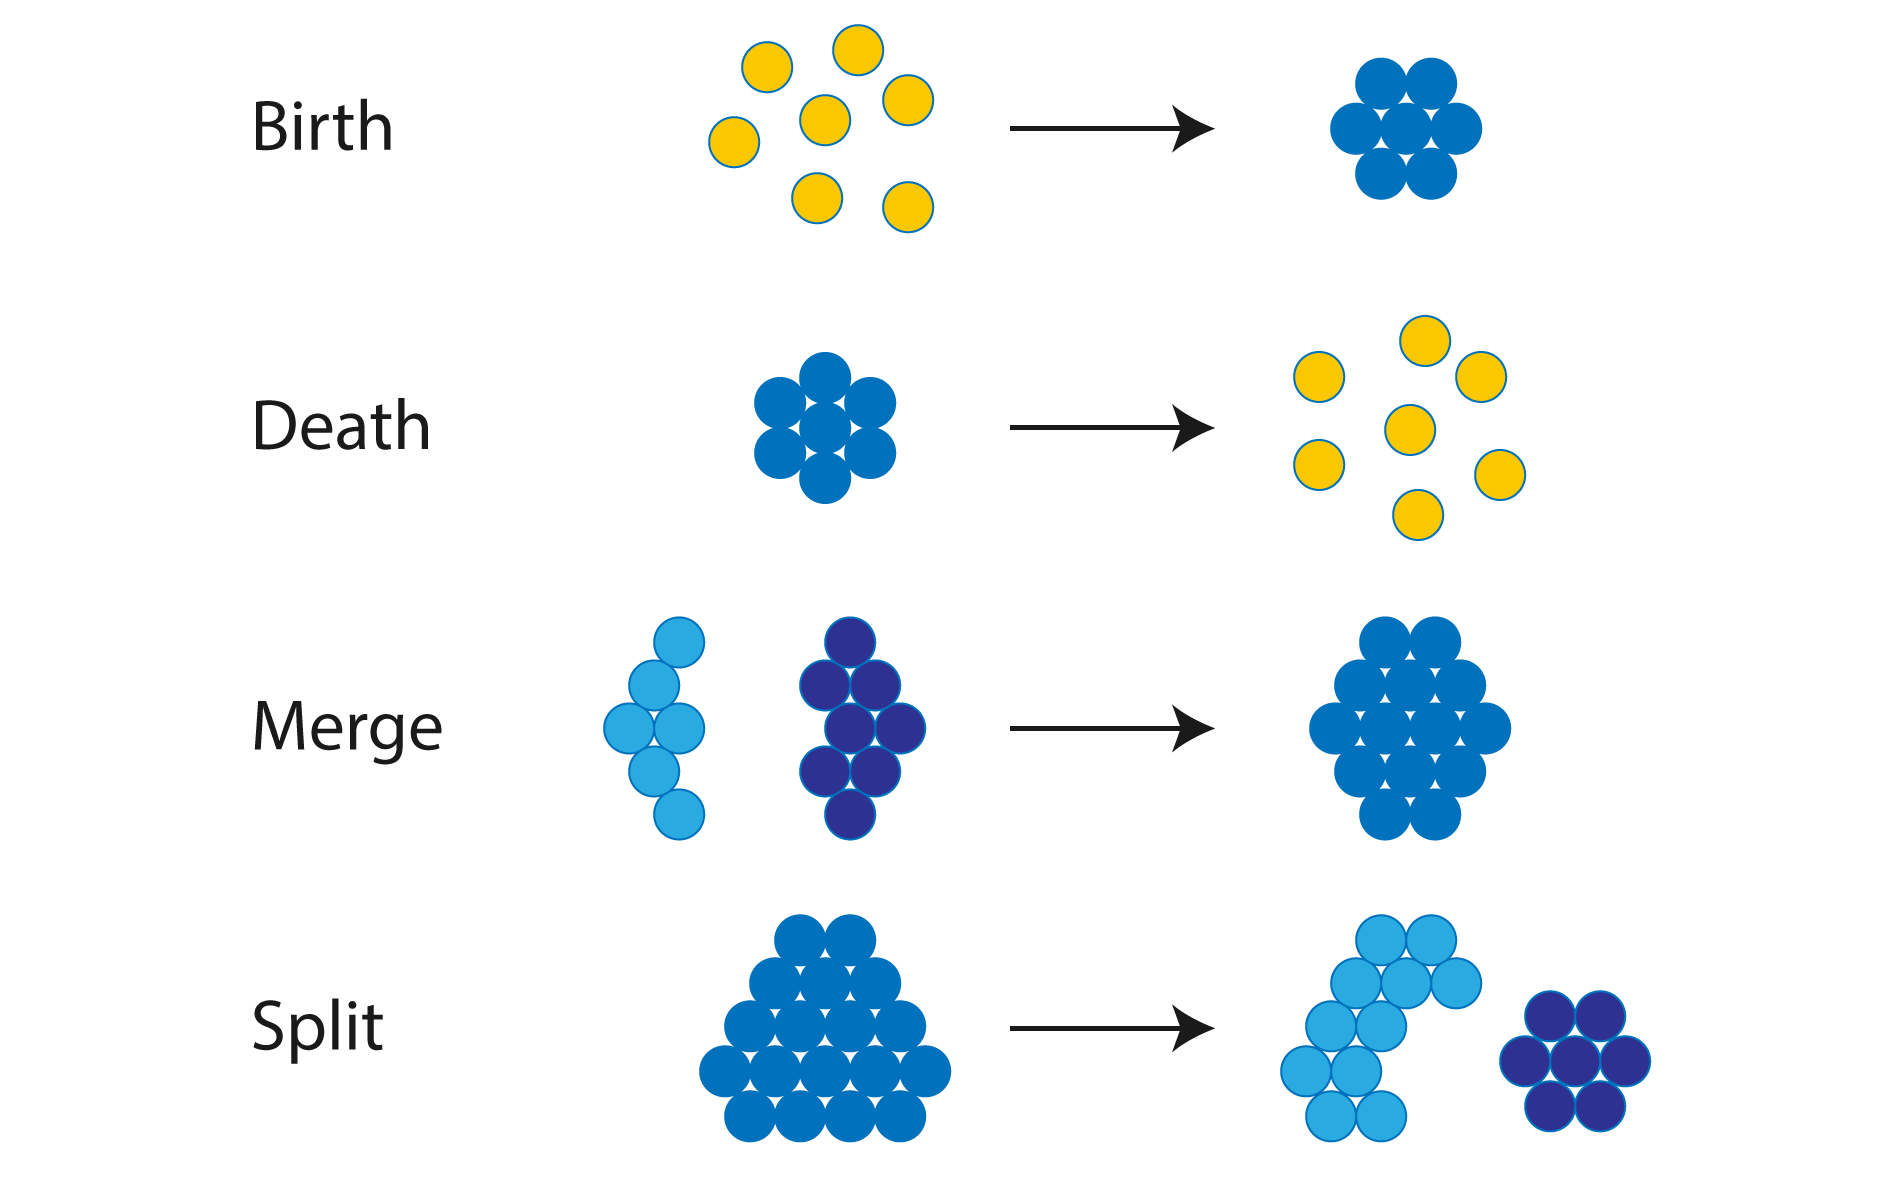
\includegraphics[width=1\textwidth]{strukturereignisse}
	\caption{Die vier Arten der Strukturereignisse: Birth, Death, Merge und Split. Die gefüllten Kreise symbolisieren Partikel. Die gelbe Füllung steht für die Gasphase, die blaue für die Flüssigkeitsphase.}\label{fig:strukturereignisse}
\end{figure}

Die Partikel liegen als diskrete Topologie, das heißt mit voneinander disjunkten Positionen vor. Bis auf die räumliche Nähe weisen sie keine Zusammenhänge auf. Jeder Partikel besitzt einen \contour{Tiefenwert}, der unter anderem markiert, ob er sich in der flüssigen oder gasförmigen Phase befindet.

Um die Bewegung der Partikel verfolgen zu können, werden sie in Gruppen eingeteilt, ähnlich der Zusammenhangskomponenten. Da jedoch auch Strukturereignisse innerhalb dieser Komponenten erkannt werden sollen, erfolgt eine wesentlich feinere Zuordnung in sogenannte Cluster. Diese Cluster können eine gesamte Zusammenhangskomponente beinhalten oder auch nur ein Teil deren sein.

Daher liegt ein Schwerpunkt der Arbeit auf der Clustererzeugung, wozu der \CFD entwickelt wurde. Er ermöglicht eine reproduzierbare Einteilung der Partikel innerhalb von Zusammenhangskomponenten, erzeugt über mehrere Zeitschritte jedoch ein \SECterm{Ereignisrauschen}, da Änderungen in der Partikelstruktur eine andere Clusterbildung zur Folge haben.

Der zweite und der dritte Schwerpunkt und auch das Ziel dieser Arbeit sind die Erkennung der Ereignisse sowie deren Visualisierung im Raum der Partikel. Die Erkennung erfolgt auf Basis eines Vergleichs der gebildeten Cluster über zwei Zeitschritte im hier entwickelten \SECC und nutzt eine heuristische Auswertung der so entstandenen Daten. Die Analyse der daraus entstehenden Daten ermöglicht die Auswahl bestimmter Parameter, die zur Steuerung der Anzahl und der Qualität der erkannten Ereignisse dienen.
Da die Partikel als dreidimensionale Kugeln dargestellt werden (siehe \autoref{fig:partikel}), soll die Ereignisdarstellung ebenfalls mit dreidimensionalen Glyphen durchgeführt werden, um die Konsistenz in der Anzeige zu erhalten. Die Erstellung eines Prototypen wird jedoch zeigen, dass Formen abseits von Kugeln, wie die im Prototyp verwendeten Polygone, eine Erkennung erschweren. So werden im Ergebnis 3D Sprites (im Folgenden als \viss{Billboards}{Billboard} bezeichnet) verwendet, die sich stark von den Partikeln abheben und damit gut sichtbar sind. Weiterhin wird eine Taxonomie für eine Verknüpfung bestimmter visueller Attribute mit den Ereignisparametern vorgeschlagen, die zur Gestaltung und Positionierung der Glyphen dient. Ein im Rahmen dieser Arbeit erstellter Renderer ermöglicht eine Filterung und Skalierung der Glyphen, so dass der Anwender die Darstellung seinen Bedürfnissen nach anpassen kann.

\begin{figure}
	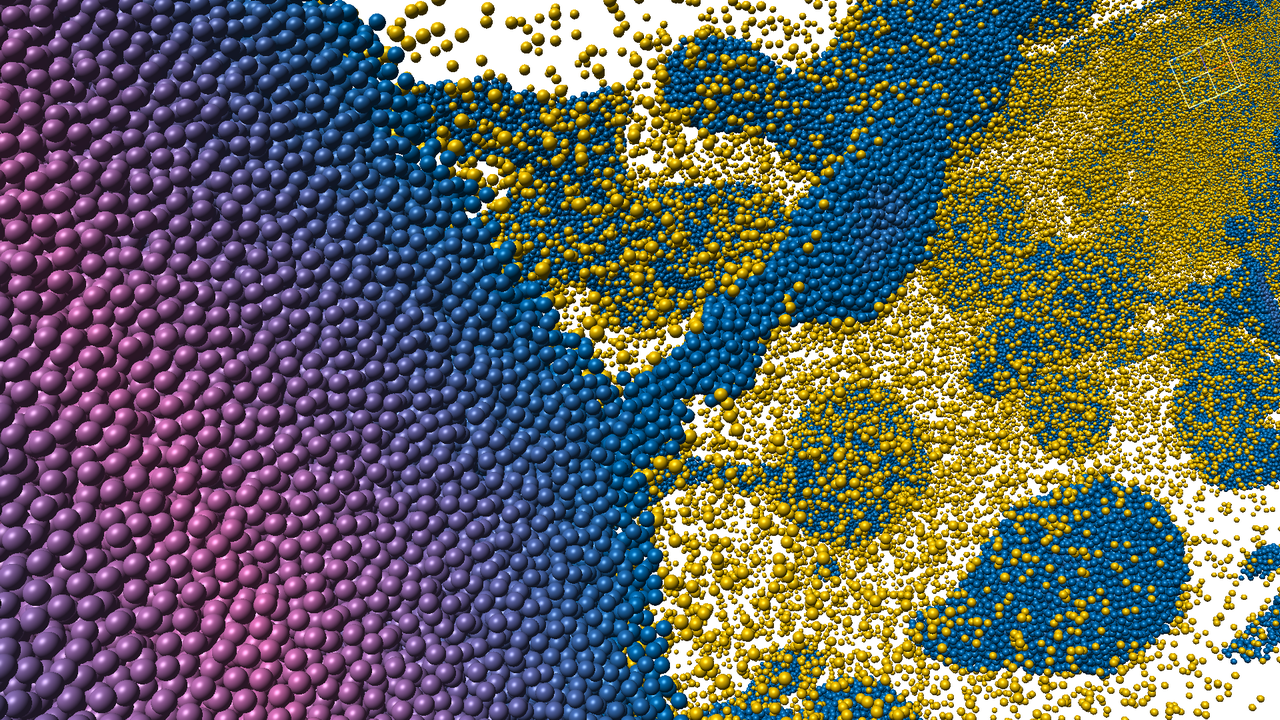
\includegraphics[width=1\textwidth]{SignedDistanceColor-Show-Frame-60-small}
	\caption{Kugelförmige Partikeldarstellung im Simulationsraum. Gelbe Partikel befinden sich in der Gasphase, blau-rote in der Flüssigkeitsphase.}\label{fig:partikel}
\end{figure}

Eine Herausforderung stellt der Ansatz für die Clusterbildung dar. Dies kann über den \contour{Tiefenwert} der Partikel kombiniert mit Abstandsmessungen geschehen oder über die Bestimmung ihrer Nachbarschaftsbeziehungen. Der Aufwand für beide Berechnungen skaliert mit $\mathcal{O}(n^2)$ mit $n$ als Partikelanzahl. %Detaillierter im Abschnitt Nachbarschaftssuche
Auch wird zu klären sein, wie die Aufteilung der Zusammenhangskomponenten in einzelne Cluster erfolgen kann. %verwandte Arbeiten/lokale MAxima helfen...
Weiterhin muss geprüft werden, ob Ereignisse durch die Untersuchung einzelner Partikel, durch topologische Veränderungen der durch die Partikel beschriebene Grenze (keine Grenzfläche, da diskrete und keine kontinuierlichen Daten vorliegen), durch die Nachbarschaften von Clustern oder über Mengenvergleiche erkennbar sind.

Dabei soll die Methodik eine akzeptable Berechnungszeit besitzen, um ihre Parameter für die Evaluation justieren zu können. Akzeptabel bedeutet, dass die Berechnungen der Cluster und der Ereignisse für einen Zeitpunkt des zwei Millionen Partikel großen Datensatzes innerhalb von Minuten und nicht von Stunden abgeschlossen sein müssen. Es wird geprüft, inwieweit Erkenntnisse aus der Skelettextraktion, der Behandlung von Laserscandaten sowie die Nutzung von \contours{Konturbäumen}{Konturbaum} bei der Entwicklung helfen können.

Zur Prüfung der Skalierbarkeit der eingesetzten Algorithmen werden quantitative Messungen mit verschiedenen Parametern verglichen. Weiterhin wird die Qualität der Ereignisermittlung durch einen visuellen Vergleich mit den Partikeldaten durchgeführt. Die der Visualisierung zugrundeliegenden Thesen hinsichtlich der Glyphgestaltung werden durch eine Umfrage geprüft, die durch wenig Erklärungen des Sachverhaltes eine unvoreingenommene Einstellung der Teilnehmer sicherstellt.



\chapter{Verwandte Arbeiten}
Für die Zuordnung von Teilchen zu Agglomerationen bzw. Zusammenhangskomponenten ist das Wissen über deren räumliche Begrenzung Voraussetzung, das Wissen über ihre Topologie. Dazu ist es notwendig, den Oberflächenverlauf oder Positionsinformationen über das Volumen zu kennen. Die Volumen- und Oberflächenbestimmung von großen Datensätzen ist bei Skelettextraktionen untersucht, die zum Beispiel die durch Laserscanverfahren ermittelte Daten auswerten. Weiterhin wurden Datenstrukturen entwickelt, um räumliche Datensätze beliebiger Dimensionen anhand ihrer Funktionswerte in Zusammenhangskomponenten einzuteilen. Sie werden als \contours{Konturbäume}{Konturbaum} bezeichnet.

Anschließend wird auf die Visualisierung großer Datenmengen eingegangen.

\section{Skelettextraktion}
Skelettextraktionsverfahren nutzen Oberflächen oder Volumen dazu, eine (volumenlose) 1D Skelettkurve zu erstellen, die die Oberfläche oder das Volumen eines 3D Objektes durch ihren Bogenverlauf abbildet und zusätzliche Eigenschaften als Metadaten enthält wie z.B. die Volumendicke \cite{au2008skeletonExtractionbyMeshContraction}. Palágyi vergleicht die Kurve mit einem brennenden Gegenstand, der von allen Seiten gleichmäßig niederbrennt. Die Stellen, an denen sich das Feuer auslöscht, bilden das Skelett des Gegenstandes \cite{palagyi2008parallelSurfaceThinning}. Blum nennt sie Medialachsenskelette \cite{blum1967descriptorsOfShape}. Daneben gibt es, abhängig vom Skelettermittlungsverfahren weitere Skeletttypen wie z.B. Kurvenskelette \cite{dey2006CurveSkeletonsMedialGeodesicFunction} \cite{cornea2007curveSkeletonProperties} oder die durch down-sampling davon abgeleiteten Knochenskelette, die vor allem in der Charakteranimation \cite{wang2007envelopingRotiationalRegression} und Netzdeformation \cite{weber2007contextAwareSkeletalShapeDeformation} eingesetzt werden.
Um Skelette aus Oberflächendaten zu berechnen, kommen zum Beispiel Voronoidiagramme zum Einsatz, mit denen der Raum in Regionen aufgeteilt wird und die mediale Oberflächen aus den inneren Kanten und Flächen des Diagramms extrahieren \cite{dey2006CurveSkeletonsMedialGeodesicFunction}. Eine Alternative ist die Nutzung des Reebgraphen, dessen Knoten die kritischen Punkte einer auf die Oberfläche angewandten reellwertigen Funktion sind, welche Topologieänderungen der Oberfläche entsprechen \cite{pascucci2007computationReebGraph}. Der Graph liegt etwa der Laplaceglättung zugrunde, bei der mehrere Eckpunkte eines Netzes zu einem Vertex zusammengefasst werden und so das Objekt verkleinert wird \cite{au2008skeletonExtractionbyMeshContraction}. Weitere Methoden sind das Ausdünnen beim Vorliegen von binären Daten (Daten mit nur zwei Intensitätszuständen, wie z.B. schwarz-weiß Bilder) durch schrittweises Entfernen der äußeren Datenpunkte \cite{palagyi2008parallelSurfaceThinning}, die Berechnung mittels mittleren Krümmungsflusses, wo die Bewegungsgeschwindigkeit der Normalen eines Punktes auf der Oberfläche vom Krümmungsradius der Oberfläche an diesem Punkt abhängt \cite{tagliasacchi2012meanCurvatureSkeletons} oder Netzzerlegungen unter Beachtung der geodätischen Abstände sowie von konvexen Verläufen und Verlinken der Komponenten \cite{katz2003meshDecomposition}.
Die Berechnung von Skeletten aus Volumendaten erfolgt ebenfalls durch Ausdünnung, etwa von Voxeln durch schrittweises Entfernen der äußeren Voxel \cite{ma2002TopologyPreservingReduction}, durch vorherige Verkleinerung der Volumenmodelle \cite{wang2008curveSkeletonExtraction} oder durch Distanzfeldmethoden, bei denen ein Distanzfeld für jeden inneren Punkt aufgebaut wird, das die Entfernung zum Rand des Objektes enthält und daraus bestimmte Voxel ausgewählt werden, die bei einer Verbindung untereinander eine mediale Oberfläche erzeugen \cite{hassouna2005robustCenterlineExtraction}. Andere Feldmethoden nutzen einen Potentialwert für innere Punkte durch Einbeziehung mehrerer Randvoxel und sind somit weniger anfällig für Rauschen, jedoch aufwändiger in der Berechnung \cite{cornea2005hierarchicalCurveSkeletons}. Diese Liste ist nur ein Auszug von üblichen Methoden. Für Kurvenskelette gibt \cite{cornea2007curveSkeletonProperties} eine umfassende Methodenübersicht.

Den Methoden ist gemeinsam, dass sie die vorhandenen Oberflächen- oder Volumendaten diskretisieren müssen, sollten sie als kontinuierliche Funktionen vorliegen, und die Daten durch eine Bewegung von außen nach innen reduzieren, wodurch eine ursprünglich große Datenmenge durch wenige Knoten repräsentiert werden kann und somit ein Einsatz vor allem in Echtzeitanwendungen findet. Die Verfahren haben dabei mit Problemen wie fehlender Wiedergabe von Oberflächenbeschaffenheiten, insbesondere bei Ausdünnungsverfahren, mit Rauschen oder mit numerischen Instabilitäten bei schlechter Datendiskretisierung zu kämpfen und benötigen teilweise umfangreiche Pre- oder Postprocessingverfahren etwa zum Entfernen von Artefakten oder zum nachträglichen Zentrieren des Skeletts \cite{cornea2007curveSkeletonProperties}.

%Die Distanzfeldmethoden bieten Möglichkeiten, den Partikelabstand zum Rand des Clusters zu bestimmen.

Für die Bestimmung der Zugehörigkeit von Partikeln des dieser Arbeit vorliegenden Partikeldatensatzes zu Agglomerationen können diese in der Skelettextraktion verwendeten Methoden nicht übernommen werden. Zum Einen basieren viele auf Netzdaten, bei denen die Punkte des Datensatzes im Gegensatz zum Datensatz dieser Arbeit miteinander in Beziehung stehen. Zum Anderen sind auch solche Verfahren ungeeignet, die als Datengrundlage vollständige Punktmengen \cite{wang2008curveSkeletonExtraction} \cite{sharf2007onTheFlyCurveSkeleton} oder bei Laserscanverfahren unvollständig ermittelte Punktmengen \cite{tagliasacchi2009curveIncompletePointCloud} verwenden. Denn die Daten werden derart reduziert, dass die für die Ereigniserkennung notwendige Wanderung von Partikeln nicht verfolgt werden kann. Hingegen ist die Idee des Reebgraphen \cite{pascucci2007computationReebGraph}, die eine auf kritische Punkte beschränkte Struktur darstellt, ein guter Ansatz für eine mögliche Einteilung der Strukturen in Cluster.

%da sie Fokus auf die Bewahrung der Oberflächentopologie legen, die bei der Erkennung von Strukturereignissen eine geringere Rolle spielt (nicht wahr, da Löcher etc doch interessieren!) und zudem Daten aus der Oberfläche und dem Volumen entfernen und damit die für die Ereigniserkennung notwendige Wanderung von Partikeln nicht verfolgt werden kann.


\section{Zusammenhangskomponenten und Konturbäume}\label{sec:related:connectedContour}

Um die Bewegung der Partikel verfolgen zu können, ist die Bildung von Zusammenhangskomponenten sinnvoll. Dabei werden Partikel zu Gruppen zusammengefasst, so dass die Wanderung von Partikeln im Verlauf der Zeit von einer zur nächsten Gruppe sichtbar wird. Diese Gruppen können mit den eingangs erwähnten Agglomerationen gleichgesetzt werden.

Zusammenhangskomponenten können bei Daten, die in einem Gitter angeordnet sind, durch Einteilung der Daten in Segmente parallel verarbeitet und damit schneller gefunden werden \cite{trevor2013efficient}. Die Erzeugung von Zusammenhangskomponenten aus Punktdaten ist über die Herstellung von Nachbarschaftsinformationen dieser Punkte möglich. Klasing et al. nutzen dabei einen definierten Maximalabstand, in dem Punkte noch als Nachbarn gelten und beschreiben eine effektive Implementation ohne die Nutzung von Baumstrukturen \cite{klasing2008efficientSegmentationOf3DLaserData}. Dies kann hier aufgrund der Erfordernis einer vollständigen Datenstruktur nicht angewandt werden. Jedoch wird in dieser Arbeit die radienbasierte Nachbarschaftssuche als Grundlage für die Clusterbildung verwendet (siehe \autoref{sec:nachbarschaftssuche}).
%Fortsetzung in Nachbarschaftssuche

\contours{Konturbäume}{Konturbaum} bieten die Möglichkeit, Datenelemente anhand ihres Funktionswertes zu gruppieren und für verschiedene Funktionswerte Zusammenhangskomponenten erkennen zu können \cite{vanKreveld1997isosurfaceTraversal} \cite{bajaj1997contourSpectrum}. Diese Flexibilität ist ihr Vorteil. Weiterhin kann mit ihnen festgestellt werden, wann die Zusammenhangskomponenten entstehen, wann sie verschwinden, sich verbinden und sterben, analog zu den mit dieser Arbeit zu erkennenden Strukturereignissen.
%Die vollständige Zuordnung von Partikeln zu Agglomerationen als auch eine benutzergesteuerte Eingabe für die Kontrolle eines Schwellwertes, ab wann Cluster als solche erkannt werden, bieten Konturbäume.
Sie sind für beliebige Dimensionen geeignet, setzen jedoch wie die Skelettextraktionsverfahren Daten in einer Netz- oder Gitterstruktur voraus, denen ein Skalarfeld zugeordnet ist. Dieses weist jedem Punkt einen Funktionswert zu.

Der \contour{Konturbaum} ist ein Graph, der die \contours{Konturen}{Kontur} von Niveaumengen im Verbinden und Entstehen oder Trennen und Sterben verfolgt. Eine Niveaumenge ist die Menge aller Punkte einer Funktion bzw. eines Skalarfeldes, denen ein gleicher Wert zugeordnet ist. Dieser Wert wird nach \cite[S.~1]{carr2010flexibleIsosurfaces} als \contour{Isowert} bezeichnet. Im Zweidimensionalen werden damit \contours{Isolinien}{Isolinie} erzeugt, im Dreidimensionalen sind es \contours{Isooberflächen}{Isooberfläche}. Sie finden zum Beispiel bei der Visualisierung von Höhendaten auf topografischen \cite{hurni2010landform} \cite{openstreetmapContours}, von Temperatur-, Wind- und Luftdruckdaten auf meteorologischen Landschaftskarten \cite{hopkins1996weather} oder von Gewebestrukturen auf Computertomographieaufnahmen \cite{tang2014ctImages} Verwendung.
Der dieser Arbeit zugrundeliegende Datensatz befindet sich in einem dreidimensionalen Raum, so dass sich auf \contours{Isooberflächen}{Isooberfläche} beschränkt wird. Diese Oberflächen schließen ein Volumen ein. Die Partikel innerhalb des Volumens bilden eine oder mehrere Zusammenhangskomponenten, die als \contours{Konturen}{Kontur} bezeichnet werden \cite[S.~2]{carr2001computingCountourTrees}.

\subsection*{Kritische Funktionswerte zur Erkennung von Konturveränderungen}
Um die Entwicklung dieser \contours{Konturen}{Kontur} zu verfolgen, ist die Erkennung sogenannter kritischer Funktionswerte notwendig, die bei einem derartigen \contour{Isowert} auftreten, bei dem sich die Topologie oder Anzahl der \contours{Konturen}{Kontur} ändert. In der Morsetheorie ist ein Punkt dann ein kritischer Punkt, wenn kein Gradient vorhanden ist  \cite{milnor1963morse} \cite{shinagawa1991surfaceBasedOnMorse}. Damit setzen die Theoreme voraus, dass sich an diesen Punkten die Topologie der Niveaumenge ändert. Bei einer abschnittsweisen linearen Funktion heißt das, wenn der \contour{Isowert} durch den Funktionswert verläuft und sich dabei die Topologie der Niveaumenge ändert, dann ist es ein kritischer Funktionswert. Alle anderen sind reguläre Funktionswerte \cite{carr2010flexibleIsosurfaces} \cite{chiang2005contourTreesUsingMonotonePaths}.

\subsection*{Abtastalgorithmus}\label{sec:related:konturAbtast}
\contours{Konturbäume}{Konturbaum} enthalten Funktionswerte in Form von Minima, Maxima und Sattelpunkten. Nicht jeder dieser Werte ist ein kritischer Funktionswert. Der \contour{Konturbaum} wird mit einem Algorithmus in vier Schritten gebildet.

Da die Daten in einem Gitter oder Netz vorliegen und ihnen ein Skalarfeld zugeordnet ist, werden sie als erstes nach ihrem des im Skalarfeld enthaltenem Funktionswert sortiert. Anschließend werden in jeweils einem Schritt zwei Bäume erstellt, indem die Punkte einmal vom kleinsten zum größten Funktionswert und ein zweites Mal vom größten zum kleinsten Wert durchlaufen werden. Die Knoten des Baumes bilden \contours{Isowerte}{Isowert}, bei denen Niveaumengen entstehen, teilen, verbinden oder verschwinden. Geschlechtsänderungen werden nicht beachtet. Die Kanten bilden äquivalente \contours{Konturen}{Kontur}. Dabei entstehen ein Verbindungs- und ein Teilungsbaum \cite{carr2001computingCountourTrees_web}. Schließlich werden im vierten Schritt beide Bäume zusammengefügt, wobei alle Knoten mit dem Grad zwei entfernt werden. Dieser resultierende Baum wird \contour{Konturbaum} genannt und die Methodik als Abtastalgorithmus bezeichnet \cite{carr2001computingCountourTrees} \cite[S.~176]{chiang2005contourTreesUsingMonotonePaths}.

%TODO Bilder Konturbaumalgorithmus: \cite[S.~1]{chiang2005contourTreesUsingMonotonePaths} Fig. 1, \cite[S.~44]{carr2010flexibleIsosurfaces} Fig. 2

Da die \contours{Konturbäume}{Konturbaum} nur kritische Funktionswerte beinhalten, sind sie eine spezielle Version der auch bei Skelettextraktionsverfahren verwendeten Reebgraphen \cite{pascucci2007computationReebGraph} für reellwertige Skalarfelder \cite[S.~44]{carr2010flexibleIsosurfaces}. Diese speziellen Reebgraphen finden auch Anwendung bei Varianten des \contours{Konturbaums}{Konturbaum}. Beispielsweise bietet das Multi-Resolution-Verfahren umfangreichere Filtermöglichkeiten durch Erweiterung des Baumes, ist jedoch auch langsamer \cite{pascucci2004multiResolutionComputation}. Hingegen ist ist ein schnelleres und speichersparenderes Verfahren der Monotonpfadalgorithmus, der nur eine für die aktuelle Betrachtung interessante Teilmenge der kritischen Werte im Baum speichert \cite{chiang2005contourTreesUsingMonotonePaths}.

Dem Abtastalgorithmus des \contours{Konturbaums}{Konturbaum}, der davon abgeleiteten Varianten sowie einiger Skelettextraktionsverfahren ist gemeinsam, dass sie kritische Werte des über den Daten liegenden Skalarfeldes nutzen, um räumliche Strukturen zu analysieren und zu speichern. Leider können diese Methoden auf den dieser Arbeit zugrundeliegenden Datensatz nicht angewandt werden. Zwar enthält der Partikeldatensatz ebenfalls ein Skalarfeld, das jedem Datenpunkt bzw. Partikel einen Funktionswert zuweist, jedoch sind keine Zusammenhänge zwischen den Partikeln bekannt. Dagegen sind die vorgestellten Methoden für in Gittern oder Netzen vorliegende Daten ausgelegt bzw. sie werden aus kontinuierlichen Flächen in beispielsweise simpliziale Netze umgewandelt. Carr fast dies in einer Arbeit zusammen:
\blockcquote[1]{carr2009representingInterpolantTopology}{[The contour tree] has been used for isosurface extraction, for abstract representation of the field, to index individual contours and their geometric properties, to guide simplification of input meshes, and to compare scalar fields.
Although recent algorithms for computing the contour tree are efficient, they were originally defined only for simplicial meshes, then extended to trilinear meshes and digital images.}
Auch aktuelle Arbeiten über \contours{Konturbäume}{Konturbaum} benutzen Netze als Grundlage \cite{raichel2014avoidingGlobalSort} \cite{acharya2015memoryEfficientCT}.

Dennoch kann ein Teil des Abtastalgorithmus als Ideengeber verwendet werden. Die Bildung des Verbindungsbaumes lässt sich auf das Ablaufen der Partikel bei der Clustersuche übertragen, indem der ihnen zugewiesene Funktionswert genutzt wird und indem zuvor Nachbarschaftsverhältnisse gebildet werden (siehe \autoref{sec:fast-depth}).

\subsection*{Temporale Betrachtungen bei Konturbäumen}\label{sec:related:konturbaumTemporal}
Der vorliegende Partikeldatensatz enthält einen Zeitverlauf über 150 Zeitschritte, der zur Ermittlung der Strukturereignisse verwendet wird. Für \contours{Konturbäume}{Konturbaum} gibt es eine Beschreibung von Laney et al über ein temporales Verfolgen von räumlichen, in einer regelmäßigen Gitterstruktur angeordneten Daten mit einem geometrischen Ansatz, der die kritischen Punkte von aufeinanderfolgenden \contours{Isooberflächen}{Isooberfläche} miteinander vergleicht \cite[S.~1056]{laney2006turbulentMixingLayer}.

Sohn und Bajaj hingegen berechnen Ähnlichkeiten von \contours{Konturbäumen}{Konturbaum} bei aufeinanderfolgenden Zeitschritten durch einen Volumenvergleich \cite{silver1997trackingTurbulent3DFeatures}. Dabei wird das von \contours{Isooberflächen}{Isooberfläche} eingeschlossene Volumen von aufeinanderfolgenden Zeitschritten verglichen, wodurch für einen festen \contour{Isowert} Änderungen der zugehörigen \contour{Isooberfläche} verfolgt werden können, die in einem sogenannten topologischem Änderungsgraph gespeichert werden \cite{sohn2006timeVaryingContourTopology}. Diese Idee kann auf den Vergleich der Cluster und die damit verbundene Ereigniserkennung angewandt werden (siehe \autoref{sec:clusterzusammenhaenge}).

Die Arbeiten von Edelsbrunner et al \cite{edelsbrunner2004timeVaryingReebGraphs} und Szymczak \cite{szymczak2005contourEvolutionInTimeDependentScalarFields} beinhalten topologische Analysen, um Zeitdaten mit Hilfe der Evolution von zeitveränderlichen Reebgraphen bzw. \contours{Konturbäumen}{Konturbaum} zu analysieren. Sie nutzen ebenfalls kontinuierliche Daten bzw. ein zeitabhängiges Skalarfeld über einem Gitter, so dass dieselben Einschränkungen für die Übertragung auf den vorliegenden Partikeldatensatz wie bei den bereits erwähnten Arbeiten über die Skelettextraktion und \contours{Konturbäume}{Konturbaum} gelten.

\section{Visualisierung großer Datenobjekte}\label{sec:related-vis}

%Aus Abschnitt Konturbäume: Es existiert eine Implementation für MolCloud, dem Vorgänger des zugrundeliegenden Frameworks MegaMol, für die Zuordnung von Teilchen zu Zusammenhangskomponenten und die Verfolgung der Wanderung zwischen diesen Komponenten. Die Berechnungen basieren auf zwei Varianten. Eine Variante berücksichtigt nur die geometrische Position der Partikel, eine andere ihre energetischen Eigenschaften, vergleichbar zum Potentialfeld bei Skelettextraktionen \cite{cornea2005hierarchicalCurveSkeletons}.
%Doof Begründung: Sie liefern jedoch unzureichende Ergebnisse, so werden beispielsweise zu viele oder zu große Cluster erkannt \cite{vis07grottel}. Auch besitzt der Benutzer keine Möglichkeit, Einfluss auf die Clustererkennung zu nehmen.

Datensammlungen haben inzwischen einen so großen Umfang, dass eine Analyse ohne Hilfsmittel nicht mehr möglich ist. Die Computervisualisierung bietet Möglichkeiten, große Datensätze so aufzubereiten, dass der Nutzer sich einen Überblick verschaffen oder gezielte Ausschnitte der Daten analysieren kann.

\subsection*{Anordnung von Datenobjekten}\label{sec:related-visAnordnung}
In der Arbeit von Gleicher et al ist eine umfangreiche Betrachtung zahlreicher Informationsvisualisierungen mit komplexen Objekten enthalten und es wird eine Taxonomie vorgeschlagen, um diese miteinander vergleichen zu können \cite{gleicher2011visualComparison}. Dabei werden die vergleichenden, visuellen Gestaltungsmethoden in die drei Grundkategorien Gegenüberstellung (Juxtaposition), Überlagerung (Superposition) und explizite Verschlüsselung (explicit encoding) eingeordnet. Weiterhin werden jeweils zwei dieser Kategorien miteinander verknüpft, so dass die Taxonomie sechs Kategorien enthält. %TODO- Bild: DB Pro Sem, erste Abb

Die Glyphdarstellung und die Darstellung der Partikel der vorliegenden Arbeit können vor allem aus Sicht der (Informations)Visualisierung als zwei getrennte Objekte betrachtet werden. Die Zielstellung ist eine Visualisierung der Partikel und \viss{Ereignisglyphen}{Ereignisglyph} im selben Raum, was der Kategorie der Überlagerung in der von Gleicher et al vorgeschlagenen Taxonomie entspricht. Möglichkeiten für die Nutzung anderer Kategorien werden in \autoref{sec:diskussion} diskutiert. %Fortsetzung in sec:visualisierung

\subsection*{Filterung von Datenobjekten}\label{sec:related-visFilter}
Um Objekte mit vielen Datenelementen auswerten zu können, bieten Informationsvisualisierungen Werkzeuge wie Filter- und Zoomtechniken. Aus Mangel an verbindlichen Regeln für Darstellungen leitet Lima, losgelöst von einschränkenden Taxonomien zur grafischen Präsentation von Daten \cite{brinton1914graphicMethods}, anhand der Analyse zahlreicher Darstellungen \cite{lima2015visualComplexity_web} Prinzipien zur Herangehensweise an Visualisierungen großer Datensätze ab \cite[S.~81-95]{lima2013visualComplexity}. Trotz dessen, dass sich diese Prinzipien auf Netzwerke konzentrieren, werden zeitliche Änderungen über die Bewegung und Veränderung von Knoten und Verbindungen vorgeschlagen analog zur Bewegung der Partikel. Genauso lässt sich die Betrachtung der Sichten übertragen. Dort betont der Autor, dass die Umsetzung einer Makrosicht und einer Mikrosicht dabei hilft, dem Nutzer sowohl eine quantitative als auch eine qualitative Erfassung zu ermöglichen. Die quantitative Erfassung dient zum Erkennen von zusammengehörigen und alleinstehenden Elementen sowie der Struktur im Ganzen. Individuelle Verbindungen zwischen den Elementen sind dabei nicht relevant. Die qualitative Erfassung dient zur Bewertung einzelner Elemente, zu detaillierten Informationen über sie und damit zur Darstellung von Fakten. %für Eva

Die Unterstützung beider Sichten wird durch die Bewegungs- und Zoomfähigkeit der Kamera des verwendeten \tool{MegaMol} Viewmoduls (siehe \autoref{sec:pluginaufbau}) grundsätzlich ermöglicht. Um dem Nutzer auch in die Lage zu versetzen, die Daten sowohl quantitativ als auch qualitativ zu erfassen, wird eine Anpassung der Größe der \viss{Ereignisglyphen}{Ereignisglyph} erlaubt.

Auch erwähnt Lima eine Beziehungssicht zur Analyse des Systems, welche die Existenz und Stärke von Verbindungen aufzeigt. Dafür wird die Nutzung mehrerer Perspektiven empfohlen. Dies kann beispielsweise mit der Kombination von Gegenüberstellung und expliziter Verschlüsselung erreicht werden (siehe \autoref{sec:related-visAnordnung}, \autoref{sec:diskussion}). %für Diskussion/Aussicht

\subsection*{Element- und Zeitdarstellung in Molekulardynamiksimulationen}

Die Molekulardynamik untersucht Wechselwirkungen zwischen Atomen und Molekülen durch beispielsweise numerische Verfahren wie Runge-Kutta. Simulationen der Molekulardynamik erzeugen große Datenmengen, da selbst bei Prozessen, die in Größenordnungen um die $10^{-9}m$ stattfinden, zahlreiche Teilchen betroffen sind und sich durch chemische Bindungen oder physikalische Stoßprozesse gegenseitig beeinflussen. Hier wird sich auf die Simulation im dreidimensionalen Raum beschränkt, zumal auch die natürlichen Prozesse selbst in dieser Dimension stattfinden. Als vierte Dimension kommt die Zeit hinzu, deren Umfang oftmals aufgrund der Komplexität der stattfindenden Prozesse auf kurze Zeiträume beschränkt ist \cite{bylaska2013extendingTimeMD}. Weiterhin werden aufgrund der eng begrenzten Simulationsräume oft periodische Randbedingungen genutzt, wie es auch in dieser Arbeit erfolgt. %Quellen? Hm, das hier ist allgemein.

Relevanz für diese Arbeit haben Visualisierungen von molekulardynamischen Simulationen im dreidimensionalen Raum, die Atome und Moleküle als geometrische Objekte repräsentieren. So finden gewundene Bänder für Monomere \cite{cohen2007proteins}, Röhren verknüpft mit Bändern für Graphen \cite{sathe2011graphene}, Röhren für Trajektoren von Daten einer Molekularsimulation \cite{grottel2014trajectories} oder für Proteinkomplexe \cite{small2013ribosomal} \cite{cao2013cancer} oder Federn für Bindungskräfte zwischen den Teilchen \cite{keesman2013springs} \cite{mcBride2013pathIntegral_web} Anwendung. Ebenfalls werden \cite{vis07grottel} Atome als Kugeln und Agglomerationen von zusammenhängenden Atomen in einer Ellipse zusammengefasst, was analog zur Darstellung der Partikel des vorliegenden Datensatzes ist. Diesen Visualisierungen gemeinsam (ausgenommen das Papier von Keesman) ist eine Farbkodierung bestimmter Eigenschaften der Elemente, was in dieser Arbeit für die Visualisierung der Cluster (siehe \autoref{sec:visualisierung:cluster}) als auch der Zeit (siehe \autoref{sec:visualisierung:glyphen} Anwendung findet.

Die Visualisierung des Zeitverlaufs erfolgt hier durch eine Bewegung der Partikel sowie durch ein dynamisches Einblenden der (statischen) \viss{Ereignisglyphen}{Ereignisglyph}. Schon vor 30 Jahren wurden in Molekulardynamiksimulationen Animationen zur Visualisierung genutzt \cite{delhaise1984computerAnimation}. Auch werden Punkt- und Liniendiagramme benutzt, in denen die Zeit auf der horizontalen Achse abgetragen ist \cite{nerukh2008temporalPatternsMD}. In Flussdiagrammen von Fluidsimulationen wird der Zeitverlauf ebenfalls in der horizontalen Richtung dargestellt \cite{laney2006turbulentMixingLayer}. Eine umfassende Aufstellung möglicher Zeitdarstellungen komplexer Daten ist in \cite{lima2013visualComplexity} zu finden.


\subsection*{Glyphdesign}\label{sec:related:glyphdesign}
%\subsubsection{Zweidimensionale Formgebung}\label{sec:related-2dformgebung}

\viss{Ereignisglyphen}{Ereignisglyph} können in dreidimensionaler oder zweidimensionaler Form erstellt werden. Durch die Nutzung eines Glyphprototypen kann in \autoref{sec:visualisierung:glyphen3d} gezeigt werden, dass dreidimensionale Glyphen ungeeignet sind, so dass hier nur auf die zweidimensionale Darstellung eingegangen wird.

Die Arbeit von Borgo et al. beinhaltet eine aktuelle Zusammenfassung zahlreicher Faktoren, die bei der Glyphdarstellung eine Rolle spielen \cite{borgo2013glyph}. So wird eine Glypheinteilung in drei Kategorien (mit drei Subkategorien) vorgestellt, wovon in dieser Arbeit ausschließlich die symbolischen Darstellung gewählt wird, da die beiden anderen Kategorien in Form der ikonischen und der Indexdarstellung physische beziehungsweise räumliche Korrelationen zum dargestellten Objekt aufweisen \cite[S.~3]{borgo2013glyph}, die bei Strukturereignissen nicht vorhanden sind. Ebenfalls Verwendung finden - in leicht abgewandelter Form - die elf aufgezählten, \viss{visuellen Variablen}{visuelle Variable} sowohl im Glyphprototyp (siehe \autoref{sec:glyphprototyp}) als auch im entwickelten Plugin. Weiterhin stellen Borgo et al. eine Veranschaulichung der Gestaltgesetze vor. Diese Gesetze helfen bei der Einordnung der Wirkung der Animation und der Glyphen (siehe \autoref{sec:grundlagen:gestaltgesetze}) sowie bei der Auswahl der \viss{visuellen Variablen}{visuelle Variable} für die \vis{Strukturereignistaxonomie}.

Für die Glyphgestaltung in \autoref{sec:visualisierung:glyphen} dienen die Arbeiten von Maguire et al. als Inspiration, da dort die Gestaltung unter Berücksichtigung des Einsatzes in großen Graphen erfolgt und jeder Glyph mehrere Daten visualisieren kann \cite{maguire2013visualCompression} sowie die Wirkung mit zahlreichen Kombinationen aufgezeigt werden \cite{maguire2012taxonomyBasedGlyphDesign}.


\chapter{Überblick}

Trotz der in \autoref{sec:related:connectedContour} beschriebenen Schwierigkeit, die vorgestellten Datenstrukturen und Methoden für diese Arbeit zu verwenden, liefern sie Ideen für die Entwicklung eigener Algorithmen. Diese Arbeit stellt diese Algorithmen vor, die es ermöglichen, in Punktdaten Strukturen zu erkennen und diese Strukturen zu nutzen, um daraus Strukturereignisse abzuleiten und sie zu visualisieren. %TODO-, evtl verwandte Arbeiten Visualisierung heranziehen

%TODO Nach Fertigstellung der Einleitung anpassen: %Die Arbeit behandelt zwei voneinander unabhängige Bereiche. Zum Einen werden Elemente eines Vektorraumes in Gruppen zusammengefasst und anhand dieser Gruppen heuristische Bestimmungen durchgeführt, zum Anderen werden diese Ergebnisse innerhalb des Vektorraumes dargestellt. Der erste Abschnitt dieses Kapitels beinhaltet Arbeiten zur Erkennung von Strukturen, der Zweite die Erstellung grafischer Elemente.

Die in \autoref{sec:einleitung} formulierten Schwerpunkte können beibehalten werden. Die Erkennung der Cluster- und Strukturereignisse wird in \autoref{sec:cluster-ereignisse} zusammengefasst behandelt, da die Schritte direkt voneinander abhängig sind. Anschließend folgt die Betrachtung der Visualisierung der Ereignisse. Sie wird in der Auswertung und Diskussion quantitativ und qualitativ bewertet, wobei auch auf den Ressourcenverbrauch der Berechnungen eingegangen wird. Der große Umfang an gesammelten Daten und die zusammenhängenden Berechnungsschritte geben Hinweise für die Nutzung und für Verbesserungen, auf die abschließend eingegangen wird.

Die Entwicklung und Berechnungen erfolgen auf handelsüblichen Computern (siehe \autoref{sec:hardware}). \tool{MegaMol} dient als Framework und bietet Klassen für das Benutzerinterface, für die Behandlung großer Daten sowie für ihre Modifizierung, Visualisierung und Speicherung. Insbesondere die annähernd verzögerungsfreie Darstellung großer Datenmengen durch Streamingmethoden sowie das Pluginsystem sind hervorzuheben. Letzteres ermöglicht eine Kombination verschiedener Datenquellen, Berechnungs- und Ausgabemodulen. Im Rahmen dieser Arbeit entstand ein Plugin unter der \gls{MIT} und enthält vier Module und eine Kommunikationsklasse. Das \MMStruktur{StructureEventsCalculation Modul} führt sämtliche, in \autoref{sec:cluster-ereignisse} beschriebenen Berechnungen durch, das \MMStruktur{StaticRenderer Modul} dient zur Visualisierung der Ereignisse (siehe \autoref{sec:renderer}), das \MMStruktur{StructureEventsDataSource Modul} sowie das \MMStruktur{StructureEventsWriter Modul} dienen zum Lesen und Schreiben der Ereignisdaten. Für den Datentransfer der Ereignisdaten zwischen den Modulen wird der \MMStruktur{StructureEventsDataCall} verwendet. Calls sind spezielle Klassen zur intermodularen Kommunikation der \tool{MegaMol} Module. Beispielhafte Programmaufbauten können in \autoref{sec:pluginaufbau} betrachtet werden. Zur effizienten Erstellung der Aufbauten dient das dem \tools{MegaMolprojekt}{MegaMol} zugehörige Werkzeug \tool{MegaMol Configurator}.

Zur Berechnung wird das Jobsystem von \tool{MegaMol} verwendet, welches es ermöglicht, die Zeitschritte eines \gls{mmpld} (das Dateiformat, in dem der dieser Arbeit zugrundliegende Datensatz vorliegt) sequentiell nacheinander und automatisiert aufzurufen. Zur Ausführung der Jobs werden \gls{XML} Dateien genutzt, die einen Aufbau von Modulen, ihrer Eigenschaften sowie von Kommunikationsklassen beschreiben. Sämtliche verwendete Bibliotheken und Werkzeuge sind thematisch in \autoref{sec:werkzeuge} aufgeführt.

%Trotz ihrer Funktionalität 

%Dateigröße von Datensätzen, Echtzeitdarstellung

\section{Beschreibung der Simulation}\label{sec:simulation}

Die dieser Arbeit zugrundeliegende Animation simuliert eine von einem Vakuum umgebenen Flüssigkeit, die rasch expandiert. Bedingt durch das quaderförmige, längliche Simulationsvolumen und der vollständigen Füllung mit Flüssigkeit in die zwei kurzen Raumrichtungen des Quaders sowie deren zentrale Positionierung, entstehen zwei Flüssigkeitsfronten, die entlang der langen Raumrichtung des Simulationsgebiets entgegengesetzt auseinander driften. Dazwischen entstehen Filamente und Tröpfchen und Gas durch sich aus den Fronten lösende Partikel und Partikelagglomerationen. Der Begriff Filament beschreibt dabei, dass es sich um Gebilde handelt, die im Vergleich zu ihrer Länge dünn sind. Tröpfchen sind von den Fronten unabhängige Gebilde mit eher kugelartiger Form. In den Leerräumen dazwischen befindet sich Gas. Die Gasphase wird dadurch definiert, dass alle Partikel große Abstände zueinander haben und sich beispielsweise gegenseitig nicht berühren.

Mit zunehmender Entfernung der Flüssigkeitsfronten zerreißen die Filamente zunehmend. Bei Zeitschritt 89 kollidieren beide Fronten miteinander, vermischen sich und driften etwa ab Zeitschritt 94 wiederholt auseinander. Das geschieht, weil das Simulationsvolumen periodische Randbedingungen aufweist. Zur Vereinfachung der Vorstellung kann der Quader als Ring betrachtet werden, auch wenn dieses Bild die Periodizität der anderen beiden Raumrichtungen nicht berücksichtigt.

Nach die Kollision bewegen sich beide Fronten in die entgegensetzte Richtung ,,zurück''. Dabei fangen sie vor der Kollision gebildete Filamente und Tröpfchen und hinterlassen ,,hinter'' sich vor allem Tröpfchen. Die Animation endet mit Zeitschritt 149, bevor sich die Fronten noch einmal begegnen. Die Visualisierung der Animation kann \href{https://www.youtube.com/watch?v=GiAkZTbgKsQ}{online in diesem Video} begutachtet werden und enthält bereits eine durch den \CFD berechnete, vererbte Einfärbung der Cluster.

%\chapter{Grundlagen}
%auf Skelett/Contour nicht eingehen, nicht verwendet.

%\section{kD Bäume}
%TODO kd Baum

%\section{Heuristik}
%TODO evtl
%TODO evtl was aus verwandte Arbeiten des Glyphdesigns hier rein





\chapter{Erkennung der Cluster und Strukturereignisse}\label{sec:cluster-ereignisse}

Zur Erkennung der Strukturereignisse ist eine Analyse der Struktur erforderlich, die in der Bildung von Clustern resultiert. Der gesamte Berechnungsprozess wird in vier Schritte unterteilt. Als erstes wird eine Partikelliste erstellt und in dieser werden Informationen über die benachbarten Partikel hinterlassen. Als nächstes werden unter Nutzung dieser Nachbarschaftsverhältnisse Cluster erstellt und anschließend diese Cluster über zwei aufeinanderfolgende Zeitschritte verglichen. Als vierter und letzter Schritt folgt die Erkennung der Strukturereignisse über eine Heuristik, die den Vergleich aus Schritt drei nutzt. Eine zusammenfassende Liste befindet sich in \autoref{sec:cluster-ereignis-schritte}.

Vor der Beschreibung der Berechnungen werden die zugrundeliegenden Daten und die genutzten Datenstrukturen erklärt.

\section{Datenbehandlung}\label{sec:datenbehandlung}

%Das zum Konturbaum vergleichbare Skalarfeld wird aus den Abstandswerten der Partikel zum Rand desjenigen Clusters gebildet, in dem sie sich befinden. Daher wird die Bezeichnung \contour{Tiefenwert} für die Werte des Skalarfeldes verwendet. Sämtliche Partikel des Datensatzes sind Teil des Skalarfeldes, auch diejenigen der Gasphase außerhalb von Clustern.

Es liegen diskrete Eingangsdaten mit Partikeln mit definierten und disjunkten Positionen vor. Bis auf die räumliche Nähe weisen sie keine Zusammenhänge auf. Weiterhin existiert ein Funktionswert für jeden Partikel in Form einer vorzeichenbehafteten Entfernungsangabe. Dieser wurde mit Hilfe der Grenzen zwischen der flüssigen Phase und dem Vakuum bzw. der Gasphase bestimmt. Anschließend wird auf dieser Basis eine vorzeichenbehaftete Distanzfunktion aufgestellt, die für alle Partikel die Entfernung zum Rand bestimmt. Somit gibt der Funktionswert die Distanz zum nächsten Partikel an, welcher auf dem Rand eines Clusters liegt. Im Folgenden wird diese Größe als \contour{Tiefenwert} eines Partikels bezeichnet.

Partikel innerhalb von Clustern besitzen einen positiven \contour{Tiefenwert}, Partikel auf dem Rand weisen den Abstand null auf, Partikel in der Gasphase, d.h. außerhalb von Clustern, haben eine negative \contours{Tiefe}{Tiefenwert}.

Die Partikel-, Cluster- und Ereignisdaten werden als eine dichtgepackte Struktur gespeichert (siehe \autoref{tab:particle}, \autoref{tab:cluster}, \autoref{tab:ereignis}). So werden nur Datentypen mit vier und acht Byte verwendet, so dass der Compiler die Struktur wegen Ausrichtungsbeschränkungen im Speicher nicht auffüllt, wie es etwa bei ein Byte großen Datentypen passieren kann \cite{raymond1994cAlignment}.

\begin{table}
	\begin{tabularx}{\textwidth}{@{}LLL@{}}
		\toprule
		Bytes & Datentyp & Beschreibung \tabularnewline
		\midrule
		0\ldots 11 & 3x float (32 bit) & Position $(x, y, z)$ \tabularnewline
		12\ldots 15 & float (32 bit) & Radius \tabularnewline
		16\ldots 27 & 3x float (32 bit) & Farbe $(r, g, b)$ \tabularnewline
		28\ldots 31 & float (32 bit) & \contour{Tiefenwert} \tabularnewline
		32\ldots 39 & uint64\_t & Identifikator \tabularnewline
		40\ldots 43 & int (32 bit) & Clusteridentifikator \tabularnewline
		44\ldots (variabel) & std::vector<uint64\_t> & Zeiger auf einen Vektor, der die Nachbaridentifikatoren enthält \tabularnewline
		\bottomrule
	\end{tabularx}
	\caption{Struktur des Partikelobjekts.}\label{tab:particle}
\end{table}

\begin{table}
	\begin{tabularx}{\textwidth}{@{}LLL@{}}
		\toprule
		Bytes & Datentyp & Beschreibung \tabularnewline
		\midrule
		0\ldots 7 & uint64\_t & Identifikator des \CFDterms{Wurzelpartikels}{Wurzelpartikel} \tabularnewline
		8\ldots 15 & uint64\_t & Anzahl an Partikeln \tabularnewline
		16\ldots 19 & int (32 bit) & Identifikator \tabularnewline
		20\ldots 31 & 3x float (32 bit) & Farbe $(r, g, b)$ \tabularnewline
		\bottomrule
	\end{tabularx}
	\caption{Struktur des Clusterobjekts.}\label{tab:cluster}
\end{table}

\begin{table}
	\begin{tabularx}{\textwidth}{@{}LLL@{}}
		\toprule
		Bytes & Datentyp & Beschreibung \tabularnewline
		\midrule
		0\ldots 11 & 3x float (32 bit) & Position $(x, y, z)$ \tabularnewline
		12\ldots 15 & float (32 bit) & Zeitpunkt \tabularnewline
		16\ldots 19 & enum (32 bit) & Ereignisart \tabularnewline
		\bottomrule
	\end{tabularx}
	\caption{Struktur des Ereignisobjekts.}\label{tab:ereignis}
\end{table}

Die Referenzen der Partikel untereinander sowie die der Partikel zu Clustern und umgekehrt werden mit Hilfe von Identifikatoren umgesetzt, die direkt in den Strukturen gespeichert sind. Dies hat Vorteile im Vergleich zur Nutzung von Zeigern als Referenz oder zur Speicherung der Objekte selbst. Letzteres erzeugt durch das Anlegen von Objektkopien Redundanz und kann daher zu inkonsistenten Daten führen. Weiterhin bedingt dies skalierend mit der Objektanzahl eine enorme Speicherbelastung und sorgte bei Tests auf dem Entwicklungssystem (siehe \autoref{sec:hardware}) zu ständigem Auslagern auf die Festplatte. Vorteile der Objektkopien sind der schnelle Zugriff auf die Daten sowie die Unabhängigkeit von Referenzen auf andere Objekte.
Die Verwendung von Zeigern ermöglicht einen unwesentlich langsameren Zugriff und es kann auf Kopien der referenzierten Objekte verzichtet werden. Allerdings darf sich bei Nutzung dieser Methode die Position der Objekte im Speicher nicht verändern, was je nach verfügbaren Ressourcen nicht garantiert werden kann und zu undefiniertem Verhalten führt. Denn es kann nicht ausgeschlossen werden, dass die Clusterliste im Speicher verschoben wird aufgrund der während der Laufzeit dynamisch allokierten und nicht vorhersagbaren Größe. So zeigen Tests %TODO Daten von createClusters_ptrAddress.log
, dass sich während der Clustererstellung die Position der Cluster im Speicher verändert, was dadurch bedingt ist, dass die gesamte Liste verschoben wird. Dies lässt sich an den ausgelesen Werten erkennen. So weist der Wert -572662307 beim Auslesen eines Integers darauf hin, dass der Speicherallokator einer Liste diesen Wert gesetzt haben könnte und was wiederrum sagt, dass sich vorher eine Liste in diesem Speicherbereich befunden haben könnte.

Um dem Problem zu begegnen, werden statt Zeigern Identifikatoren eingesetzt. %TODO Siehe ID im Schema Partikel/Clusteraufbau
Diese Identifikatoren werden genutzt, um zur Referenzierung auf die Listenzeiger zurückgreifen zu können. Die Methode hat drei Vorteile. Erstens ist die Geschwindigkeit nicht langsamer als mit einer direkten Zeigerreferenz, zweitens verweisen die Referenzen auch bei einer Verschiebung der die Objekte enthaltenen Listen im Speicher noch auf die korrekten Objekte und drittens kann geprüft werden, ob die Referenz mit dem im Speicher befindlichen Objekt übereinstimmt. Diese Prüfmöglichkeit ist dann wichtig, wenn die Objektlisten umsortiert werden. Zum Beispiel durch das Hinzufügen oder Entfernen von Elementen, die sich nicht am Ende der Liste befinden.


\section{Schritt 1: Bestimmung der nächsten Nachbarn}\label{sec:nachbarschaftssuche}

Ausgehend von der in \autoref{sec:related:connectedContour} referenzierten Bestimmung von Zusammenhangskomponenten über einen Maximalabstand zwischen Punkten im Netz, der ohne Baumstrukturen auskommt, könnte hier ebenfalls eine radialbasierte Nachbarschaftsbeziehung verwendet werden. Diese wurde geprüft und aufgrund des hohen Zeitaufwandes, verursacht durch die Entfernungsbestimmung zwischen Partikeln, verworfen (siehe \autoref{sec:cluster-radial}).

Eine Einteilung des Raumes in ein Gitter abhängig des Partikelradius wäre eine weitere Option. Einen ähnlichen Ansatz nutzt der kD-Baum, der die Partikel abhängig von ihrer Position in seine Äste verteilt und dadurch die Suche nach benachbarten Partikeln stark beschleunigt. Die Nutzung des Baumes bietet sich an, da die Anzahl der Partikel und ihre Positionen sich während eines Zeitschrittes nicht verändern und der Baum somit nicht modifiziert werden muss. Der Baum hat aufgrund der drei Raumrichtungen die Dimension $k=3$. Die Identifikation der Partikel erfolgt über den im kD-Baum eingetragenen Index, der der Position der Partikel in der Partikelliste entspricht. Daher wird während der Laufzeit über den beim Partikel gespeicherten Identifikator überprüft, ob die Reihenfolge der Liste modifiziert wurde, um Falschzuweisungen registrieren zu können.

Die periodischen Randbedingungen des Datensatzes werden standardmäßig beachtet, indem die Nachbarschaftssuche für jeden Partikel achtmal durchgeführt wird. Dabei wird die Position des Partikels für jede Raumrichtung auf die gegenüberliegende Seite des Simulationsvolumens versetzt, was bei drei Raumrichtungen acht Kombinationen ergibt.
Für Datensätze ohne periodische Randbedingungen kann der Nutzer dieses Vorgehen deaktivieren, so dass nur die Originalposition des Partikels verwendet wird.

\tool{MegaMol} stellt mit der \ANN eine Bibliothek für die Nutzung von kD-Bäumen bereit. Von dieser wird die radienbasierte Suche annkFRsearch verwendet, da sich so eine Reichweite bestimmen lässt (siehe \autoref{sec:related:connectedContour}). Als Suchparameter werden neben des Radius' selbst auch eine maximale Anzahl von zu prüfenden Nachbarn festgelegt. Dies ist nötig, da die \ANN die Größe des Containers zur Speicherung der Identifikatoren der festgestellten Nachbarn (Nachbarschaftsliste) im Voraus festlegt. Dieser Wert wird abhängig vom Radius durch die Berechnung automatisch gesetzt. Die passenden, in \autoref{tab:maxNeighbours} aufgeführten Werte wurden experimentell bestimmt und erfüllen die beiden Voraussetzungen, dass alle im durch den Radius definierten Volumen befindlichen Artikel in die Nachbarschaftsliste aufgenommen werden können und andererseits möglichst wenig zusätzlicher, unnötiger Speicherplatz für den bei der Suche verwendeten Container für das Aufnehmen der Nachbarn reserviert wird. 

\begin{table}
	\begin{tabularx}{\textwidth}{@{}LL@{}}
		\toprule
		Partikelradiusmultiplikator & Maximal erfassbare Nachbarn \tabularnewline
		\midrule
		4 & 35 \tabularnewline
		5 & 60 \tabularnewline
		6 & 100 \tabularnewline
		7 & 155 \tabularnewline
		10 & 425 \tabularnewline
		20 & 3270 \tabularnewline
		\bottomrule
	\end{tabularx}
	\caption{Experimentell ermittelte Werte für die maximal zu erfassenden Nachbarn, damit alle Partikel innerhalb des durch den Radiusmultiplikator vorgegebenen Suchvolumens erfasst werden.}\label{tab:maxNeighbours}
\end{table}

Bei der Bestimmung wurde ein empirisches Annäherungsverfahren genutzt, in welcher die Anzahl der hinzugefügten Nachbarn bei gleichbleibendem Radius überprüft wurde. Dabei wurde mit kleinen Werten für die maximal erfassbaren Nachbarn begonnen und dieser Wert stückweise erhöht. So lange die Gesamtanzahl der zu den Partikeln hinzugefügten Nachbarn stieg, war die Anzahl an erfassbaren Nachbarn zu klein. Sobald die Nachbarn identisch blieben, war der optimale Wert gefunden. Aus Effizienzgründen wurde dieser Wert sowohl aus großer als auch als kleiner Richtung überprüft, um schneller den optimalen Wert zu erreichen.

Der Suchradius wird durch den Nutzer einstellbar gestaltet, da mit der Reichweite der Nachbarschaftssuche die Anzahl der Cluster und damit die gesamte Berechnung beeinflusst wird (siehe \autoref{sec:eva:nachbarschaftssuche}). Der Parameter wird dabei mit dem Partikelradius multipliziert, so dass die Bezeichnung \CFDterm{Partikelradiusmultiplikator} gegeben wird.

Die Suche wird für jeden Partikel durchgeführt. Dabei werden die Identifikatoren der gefundenen Nachbarn in die dafür vorgesehene Liste jedes Partikelobjekts hinzugefügt (siehe \autoref{sec:datenbehandlung}). Zuvor werden alle Partikel des \gls{mmpld} aus dem eingehenden \gls{mpdc} in diese Partikelobjekte umgewandelt und in die Partikelliste geshrieben. Da bekannt ist, wieviele Elemente der \gls{mmpld} enthält, findet eine Speicherplatzreservierung der Partikelliste statt, um eine Reallokation während der Eintragung der Partikel zu vermeiden.

Mit der Erzeugung dieser Partikelliste, der Eintragung aller Partikel in den kD-Baum und der Eintragung der Nachbarn in die Partikelobjekte ist der erste Schritt für die Berechnung der Strukturereignisse abgeschlossen und es folgt die Clusterbestimmung.

\section{Schritt 2a: Cluster-Fast-Depth Algorithmus zur Bestimmung der Cluster}\label{sec:fast-depth}

Zur Clusterbestimmung wurde der \CFD entwickelt. Der Begriff wurde ausgehend von der Nutzung des \contours{Tiefenwertes}{Tiefenwert} gewählt, angelehnt an die Depth-First Suche in Baumstrukturen.

Da auch Verschmelzungen und Teilungen innerhalb von Zusammenhangskomponenten erkannt werden sollen, genügt es nicht, wenn die Clusterbildung alle benachbarten Partikel einer Gruppe zuordnet wie in \autoref{fig:cluster-tropfen} abgebildet. Vielmehr sollen auch Zusammenhangskomponenten selbst unterteilt werden. Diese Idee ist in \autoref{fig:cluster-zusammenhang} visualisiert.

\begin{figure}
	\ffigbox[\FBwidth] {
		\begin{subfloatrow}
			\vbox {%
				\ffigbox[\FBwidth][\FBheight]
				{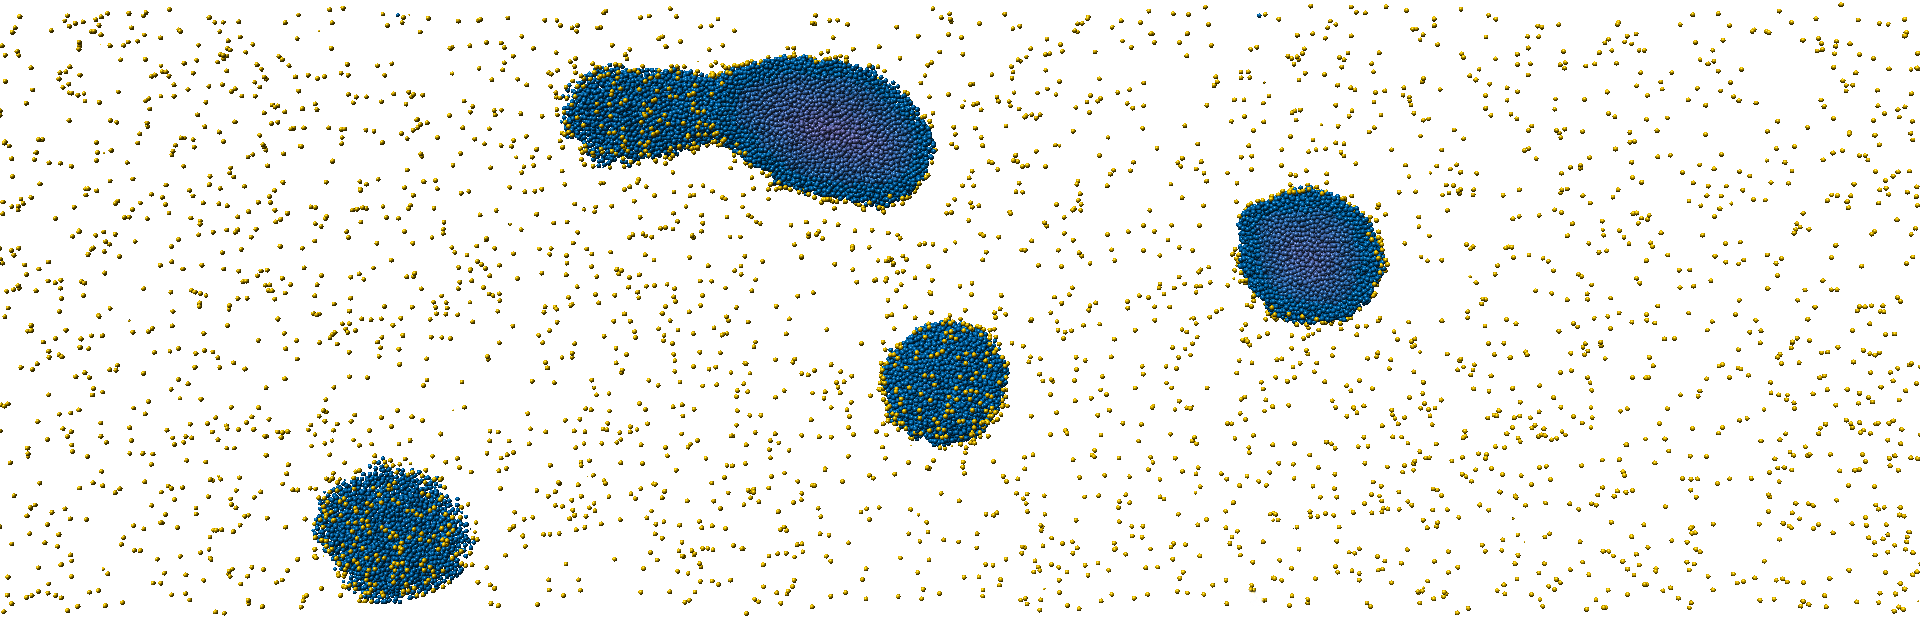
\includegraphics[width=1\textwidth]{cluster/SignedDistanceColor-Frame-090-clipplane20-letterbox}}
				{\caption{Tröpfchen separat verteilt im Raum.}\label{fig:cluster-tropfen-roh}}\vss
				\ffigbox[\FBwidth][\FBheight]
				{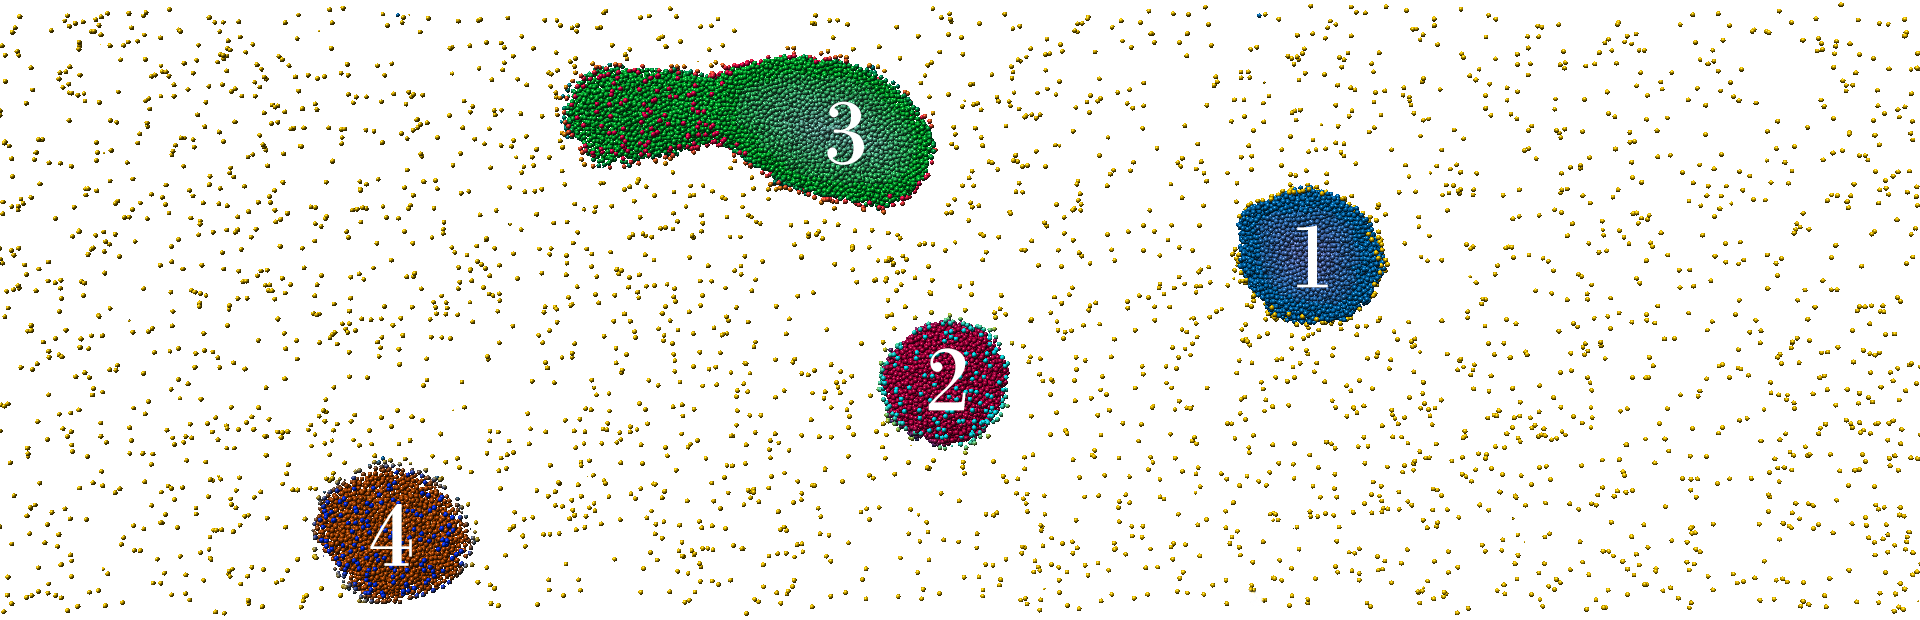
\includegraphics[width=1\textwidth]{cluster/SignedDistanceColor-Frame-090-clipplane20-letterbox-Cluster}}
				{\caption{Einfärbung der Tröpfchen zum Zeigen einer möglichen Clusteraufteilung. Die Einfärbungen und die Zahlen eins bis vier markieren dabei jeweils einen Cluster. Trivia: Cluster drei würde vom \CFD in mehrere Cluster eingeteilt werden aufgrund der Einschnürung in der Mitte.}\label{fig:cluster-tropfen-farbe}}
			}
		\end{subfloatrow}
	}
	{\caption{Ein Cluster füllt jeweils eine gesamte Zusammenhangskomponente. Zu sehen sind Tröpfchen (blau) in einem Ausschnitt der Simulation bei Zeitschritt 90. Gelbe Partikel befinden sich in der Gasphase.}\label{fig:cluster-tropfen}}
\end{figure}

\begin{figure}
	\ffigbox[\FBwidth] {
		\begin{subfloatrow}
			\vbox {%
				\ffigbox[\FBwidth][\FBheight]
				{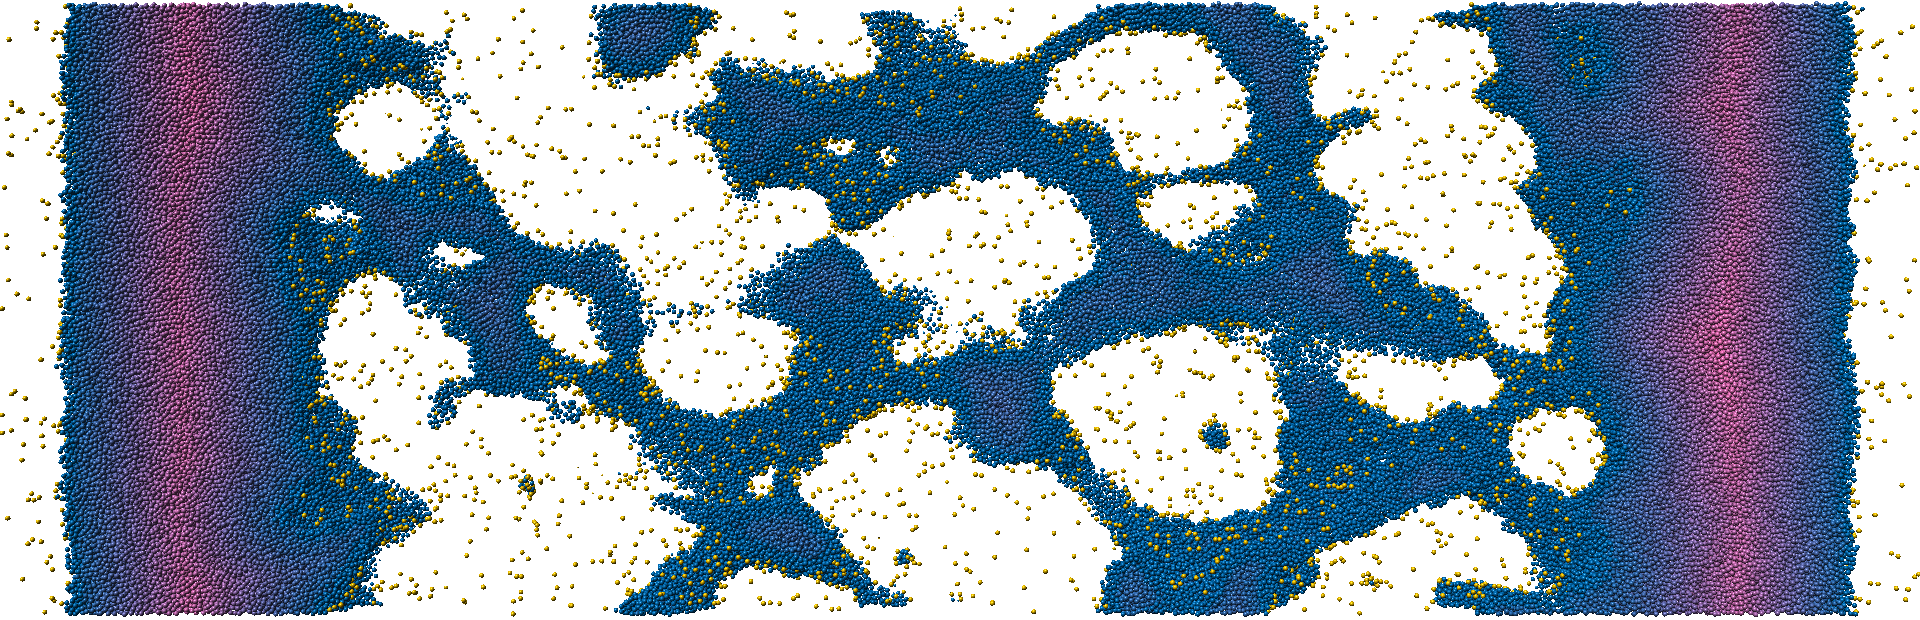
\includegraphics[width=1\textwidth]{cluster/SignedDistanceColor-Frame-016-clipplane20-letterbox}}
				{\caption{Filamentstrukturen innerhalb einer Zusammenhangskomponente zwischen den beiden Flüssigkeitsfronten.}\label{fig:cluster-zusammenhang-roh}}\vss
				\ffigbox[\FBwidth][\FBheight]
				{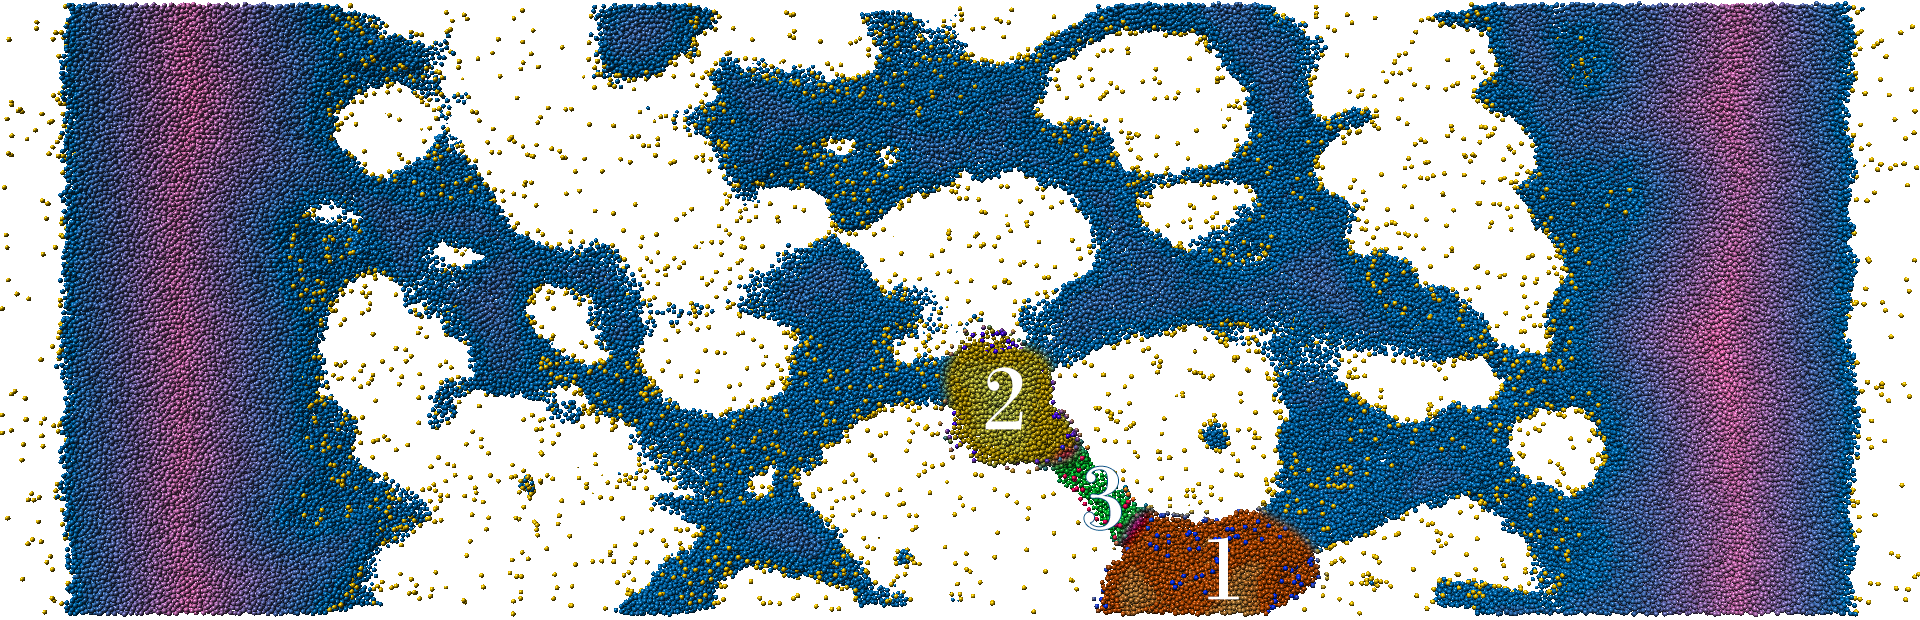
\includegraphics[width=1\textwidth]{cluster/SignedDistanceColor-Frame-016-clipplane20-letterbox-Cluster}}
				{\caption{Das Ziel ist, Partikel auch innerhalb von Zusammenhangskomponenten in Cluster aufzuteilen. Die Einfärbungen und die Zahlen eins bis drei markieren dabei jeweils einen Cluster.}\label{fig:cluster-zusammenhang-farbe}}
			}
		\end{subfloatrow}
	}
	{\caption{Clusteraufteilung innerhalb einer Zusammenhangskomponente. Zu sehen ist ein Schnitt durch den Simulationsraum bei Zeitschritt 16. Gelbe Partikel befinden sich in der Gasphase.}\label{fig:cluster-zusammenhang}}
\end{figure}

Dabei wird die Idee des Reebgraphen sowie die Bildung des Verbindungsbaumes beim Abtastalgorithmus der \contours{Konturbäume}{Konturbaum} (siehe \autoref{sec:related:konturAbtast}) aufgegriffen und es werden kritische Punkte im Skalarfeld aller Partikel gesucht. Im Gegensatz zu den beiden genannten Ansätzen, wird die Suche auf lokale Maxima beschränkt. Dies erfüllt die Anforderung, Partikel einer Zusammenhangskomponente in Gruppen zu unterteilen und ermöglicht zudem eine hohe Geschwindigkeit.

Die Partikelliste wird iterativ durchlaufen. Dabei werden die bei der Nachbarschaftssuche erstellten Beziehungen zwischen Partikeln genutzt, um für jeden Partikel denjenigen Nachbarn zu finden, der den höchsten \contour{Tiefenwert} aufweist. Ist dieser Nachbar gefunden, werden für diesen noch einmal alle Nachbarn nach dem ,,tiefsten'' durchsucht und dasselbe für diesen Partikel durchgeführt. Diese Suche geschieht ebenfalls iterativ. Sobald die umliegenden Partikel nur noch den gleichen oder einen geringeren \contour{Tiefenwert} als den des zuletzt betrachteten Partikels aufweisen, gilt die Suche als abgeschlossen. Anschließend wird ein neuer Cluster erstellt mit diesem Partikel als \CFDterm{Wurzelpartikel}. Sollte bereits ein Cluster mit diesem Partikel als Wurzel existieren, so wird kein neuer Cluster erstellt. Danach werden der ursprüngliche Partikel als auch alle Partikel, die während des iterativen Ablaufs der tiefsten Nachbarn getroffen wurden, zum Cluster hinzugefügt. Dies geschieht, indem der Clusteridentifikator des neu erstellten oder bereits vorhandenen Clusters in das Referenzfeld der Partikel für ihren zugehörigen Cluster (siehe \autoref{sec:datenbehandlung}) eingetragen wird. TODO HIER KOMMT EIN SCHEMA HIN %TODO Schema mit Illustrator erstellen analog zum Vortrag

Die Traversion erstellt einen kürzesten Pfad vom Ausgangspartikel zum Partikel mit der größten, lokalen Tiefe, wovon sich der Name für diesen Algorithmus ableitet. Da alle bei der Traversion getroffenen Partikel zum Cluster hinzugefügt werden und Partikel, kann der Algorithmus beschleunigt werden. Bevor die Fast-Depth Suche begonnen wird, wird der aktuell betrachtete Partikel auf seine Clusterzugehörigkeit geprüft. Sollte er einem Cluster angehören, so wird die Suche nicht erst begonnen, sondern es wird zum nächsten Partikel gesprungen.

Weiterhin werden Gaspartikel anhand ihres \contours{Tiefenwertes}{Tiefenwert} erkannt und übersprungen. Auch Partikel ohne Nachbarn werden übersprungen. Diese Überprüfung scheint redundant, jedoch können bei sehr kleinen Suchradien der Nachbarschaftssuche auch Flüssigkeitspartikel keine Nachbarn aufweisen, deren fehlende Nachbarschaft dann die Bedingung für Cluster, einer Zusammenhangskomponente anzugehören, nicht erfüllen würde.

Damit ist der wesentliche Teil der Clusterbildung abgeschlossen. Der zweite Schritt beinhaltet lediglich noch eine Reduktion kleiner Cluster. Die Definition für kleine Cluster kann dabei vom Nutzer getroffen werden.

%Obsolet
%Keine Sortierung wie beim vorgestellten Konturbaum. Sie ist teuer und würde den \CFDterm{Fast-Depth-Algorithmus} nicht beschleunigen. Stattdessen werden auf dem Pfad getroffene Partikel zum Cluster mit hinzugefügt.


\section{Schritt 2b: Reduzierung der kleinen Cluster}\label{sec:clusterreduktion}

Sehr kleine Cluster in den Zusammenhangskomponenten können unerwünschtes Rauschen in der Ereigniserkennung verursachen, so dass deren Partikel benachbarten, größeren Clustern zugewiesen werden. Ausgenommen sind diejenigen Cluster, die alleinig eine Zusammenhangskomponente bilden, auch wenn sie die Mindestgröße unterschreiten.

Es könnte eine Menge aus diesen sehr kleinen Clustern gebildet werden. Mit jedem Cluster diese Menge werden die naheliegensten ,,großen'' Cluster gesucht, zum Beispiel durch Anordnung der Rootpartikel der Cluster in einem kD-Baum. Allerdings ist eine Prüfung, ob sich die Cluster in einer Zusammenhangskomponente befinden, sehr aufwändig.

Aufgrund dessen, dass sich in der Arbeit auf eine kleine Mindestclustergrößen von zehn Partikeln beschränkt wird, kann eine iterative Prüfung auf benachbarte, große Cluster unter Nutzung der bestehenden Nachbarschaftsbeziehungen der Partikel genutzt werden. Dabei werden bei jedem Partikel, der ein Flüssigkeitspartikel mit Nachbarn ist und dessen referenzierter Cluster die Mindestclustergröße unterschreitet, die Nachbarn durchsucht. Sollten die Nachbarn alle keinem, demselben oder einem anderen sehr kleinen Cluster angehören, wird mit ihren Nachbarpartikeln die selbe Suche durchgeführt. In der aktuellen Implementation wird diese Suche maximal dreimal durchgeführt, so dass ausgehend vom ursprünglich betrachteten Partikel der maximal drittentfernteste Nachbar nach anderen Cluster durchsucht wird. Sollten zuvor schon andere Cluster gefunden worden sein, wird die Suche bereits dort abgebrochen. Nachbarpartikel, die keinem Cluster angehören (hier vor allem Gaspartikel, siehe \autoref{sec:fast-depth}), werden übersprungen.

Sollte nach Abschluss dieser Suche kein anderer, ,,großer'' Cluster gefunden sein, wird der sehr kleine Cluster bestehen gelassen, da dann davon ausgegangen wird, dass der Cluster eine Zusammenhangskomponente bildet und daher mit keinem anderen Cluster verschmolzen werden kann. Diese Annahme ist für eine Mindestclustergröße von zehn berechtigt, denn bei der dichten Struktur der Partikel in der Flüssigkeit erreicht spätestens die zweite Nachbarschaftsebene diese Anzahl an Partikeln. Der dritte Suchlauf dient als Puffer für etwas größere Mindestclustergrößeneinstellungen.

Sollte ein Cluster gefunden worden sein, so wird der betrachtete Partikel diesem Cluster zugeordnet. Die getroffenen Nachbarn werden nicht hinzugefügt, um die Schleife in mehreren Prozessen ohne Mutex ablaufen lassen zu können. Sollten mehrere Cluster gefunden worden sein, wird eine Entscheidung anhand der Richtung des Partikels zu den benachbarten Clustern bestimmt. Er wird zu demjenigen Cluster hinzugefügt, der am nächsten zur Richtung des Partikels zum \CFDterm{Wurzelpartikel} seines Clusters liegt.

Dazu wird der Winkel zwischen der Richtung vom \CFDterm{Wurzelpartikel} des betrachteten Partikel und seiner Position zur Richtung des Partikels zum in Frage kommenden Cluster berechnet. Dies wird für alle benachbarten Cluster durchgeführt. Der benachbarte Cluster mit dem geringsten Winkel im Intervall $[0, \pi]$ wird der neue Cluster des Partikels.

Da die Partikel voneinander unabhängig sind, können sie parallel durchlaufen werden (Umsetzung mittels \tool{OpenMP}). Weiterhin wird die Winkelberechnung zu jedem benachbarten Cluster parallelisiert.
Die Cluster werden nicht aus der Clusterliste gelöscht, um die Referenzen auf die Liste nicht neu erstellen zu müssen. Stattdessen wird durch den Algorithmus ihre Partikelanzahl auf 0 reduziert (sollten alle Partikel neuen Clustern zugeordnet werden), so dass sie in den folgenden Schritten herausgefiltert werden können.

\section{Schritt 3: Bestimmung der Clusterzusammenhänge}\label{sec:clusterzusammenhaenge}
Zur Bestimmung der Ereignisse ist es notwendig, die Entwicklung der Cluster zu verfolgen. Dazu werden Cluster über zwei Zeitschritte hinweg miteinander verglichen. Dieser Berechnungsschritt wird als \SECC bezeichnet.

\subsection*{Clusternachbarschaftsgraph}
Eine Variante ist die Erzeugung eines Graphen, der den Zusammenhang zwischen den Clustern zeigt und die bestehenden Nachbarschaftsbeziehungen der Partikel nutzt. Dazu kann die Clusterzugehörigkeit der Nachbarn jedes Partikel untersucht werden. Sollte ein Nachbar einem anderen Cluster angehören als der aktuelle Partikel, so sind der Cluster des aktuellen und der Cluster des benachbarten Partikels zusammengehörig. Durch Begrenzung auf Partikel mit geringen \contours{Tiefenwerten}{Tiefenwert} kann diese Suche stark beschleunigt werden und dennoch alle Nachbarschaftsbeziehungen gefunden werden, da einerseits der \CFD vor allem in die Tiefe und wenig in die Breite sucht und andererseits diese Beziehungen zwischen zwei Clustern aus beiden Richtungen geprüft werden.
Weiter soll darauf nicht eingegangen werden, da die Schwierigkeit dieser Variante in der Clusteridentifizierung über Zeitschritte hinweg besteht. Der Rootpartikel ändert sich von Zeitpunkt zu Zeitpunkt, die Partikelzugehörigkeit der Cluster ebenfalls (siehe \autoref{sec:eva:ereignisse}). Sie könnte als Ergänzung des hier implementierten Clustervergleichs dienen (siehe \autoref{sec:disc:optimierungAlg}.

\subsection*{Vergleich der zugehörigen Partikelmengen}
Ein direkteres Vorgehen, das unabhängig der Nachbarschaftsbeziehungen von Clustern ist, bietet der Vergleich der Partikelmengen der Cluster. Diese Methode greift die Idee des Volumenvergleichs für \contours{Isooberflächen}{Isooberfläche} von \contours{Konturbäumen}{Konturbaum} auf \autoref{sec:related:konturbaumTemporal}. Die Cluster nehmen dabei die Position der \contours{Konturen}{Kontur} ein und die Partikel die Position des Gitters, da sie über ihren Identifikator eindeutig zugeordnet werden können. Weil hier keine kontinuierliche Fläche existiert, wird nicht von eingeschlossenem Volumen, sondern von Mengen gesprochen.

Zu jedem Cluster ist eine disjunkte Menge an Partikeln zugeordnet. Um diese Mengen über zwei Zeitschritte hinweg miteinander zu vergleichen, wird eine Matrix aufgebaut, deren Zeilen die Cluster des neuen Zeitschrittes enthalten und deren Spalten die Cluster des alten Zeitschrittes. Ein Partikel wird in diese \SECterm{Clustervergleichsmatrix} eingetragen, indem die Clusterzugehörigkeit des aktuellen Zeitschrittes sowie die Clusterzugehörigkeit des vorherigen Zeitschrittes ermittelt wird.

Anschließend werden zwei Schritte durchgeführt, um die für die Auswertung und schließlich die für die Eventerkennung notwendigen Werte zu ermitteln. In jedem Schritt werden alle Cluster eines Zeitschrittes betrachtet und für jeden werden Cluster des anderen Zeitschrittes gesucht, die mit dem betrachteten Cluster gemeinsame Partikel aufweisen. Diese werden als \SECterm{Partnercluster} oder Partner bezeichnet. Im ersten Schritt werden alle Cluster des vorherigen Schrittes mit jedem des aktuellen Zeitschrittes verglichen (vorwärtsgerichteter Vergleich), im zweiten Schritt alle derzeitigen mit jedem Cluster des vorherigen Zeitschrittes (rückwärtsgerichteter Vergleich). 

Zur Speicherung der Vergleichsergebnisse wird eine Partnerclusterstruktur eingeführt. Diese enthält eine Liste der \SECterm{Partnercluster} zusammen mit den jeweils gemeinsamen Partikeln sowie Methoden zur Berechnung von Gesamt- und Durchschnittswerten. Für beide Vergleichsrichtungen werden diese Strukturen in separate Listen geschrieben. Damit lassen sich die Anzahl der gemeinsamen Partikel für jeden vorhergehenden Cluster und jeden aktuellen bestimmen, woraus sich die weiteren für die Analyse notwendigen Werte ermitteln lassen.

\section{Schritt 4: Erkennung von Ereignissen}\label{sec:ereigniserkennung}

Es wird jeweils ein Cluster und seine \SECterm{Partnercluster} betrachtet. Dies geschieht sowohl für den vorwärtsgerichteten als auch den rückwärtsgerichteten Vergleich.

Zur Analyse der durch die Partnerclusterstruktur zurückgegeben Daten wird ein heuristisches Vorgehen genutzt. Tests haben gezeigt, dass die Partikel selten in Clustern mit derselben Clusternummer bleiben. Das lässt sich damit erklären, dass die Clusterzuweisung stark von der Position der Partikel und ihrer Nachbarschaftsverhältnisse abhängen und diese sich durch die sich bewegenden Partikel von Zeitschritt zu Zeitschritt stark ändern. Somit ist der intuitiv wirkende Vergleich über den Clusteridentifikator für die Beobachtung von Veränderungen nicht möglich und kann ausgeschlossen werden. %TODO-- Testdaten Änderung Clusternummern
Dagegen kann ein Vergleich der Anteile von Partikeln in den Clustern erkennen lassen, ob sich der Zusammenhang zwischen den Partikeln verändert hat. Die für die Betrachtung relevante Clustereigenschaft ist die Anzahl der Partikel eines Clusters und wird als \SECterm{Clustergröße} bezeichnet.

Die Größe eines Clusters hat für die Gewichtung von Ereignissen keine Bedeutung, da sie durch die Vorgehensweise der \CFD stark von der Topologie der Strukturen abhängt. Ein durch einen kleinen Cluster an einer Engstelle eines Filaments ausgelöstes Ereignis kann für die Analyse bedeutender sein als ein Ereignis innerhalb der Flüssigkeitsfront, ausgelöst durch große Cluster. Um die Abhängigkeit der Ereigniserkennung von der \SECterm{Clustergröße} zu eliminieren, werden relative Werte verwendet. Das heißt, die Methoden der Strukturen des \SECC geben Werte im Verhältnis zur Größe der Cluster an. Dazu zählen der Anteil der gemeinsamen Partikel aller \SECterm{Partnercluster}, der Anteil für jeden einzelnen Partner, der Durchschnittsanteil der gemeinsamen Partikel für alle Partner sowie Maxima und Minima als auch die Anzahl der Partner.

Um festzustellen, ob ein Cluster einen ähnlichen Vorgänger oder Nachfolger hat, können der durchschnittliche Anteil der gemeinsamen Partikel über alle Partner, der Anteil des größten Partners im Vergleich dazu sowie die Gesamtanzahl der Partner herangezogen werden. Sollten die ersten beiden Werte hoch und der dritte Wert klein sein, kann mit einer zu bestimmenden Wahrscheinlichkeit in Abhängigkeit von den drei Werten davon ausgegangen werden, dass es sich um denselben Cluster handelt. Für die Erkennung der Ereignisse ist es aufgrund der oben genannten Fluktuation der Partikel zwischen Clustern jedoch nicht relevant, ob ein Cluster einen direkten Vorgänger hat. Es zeigt jedoch ein schlechtes Beispiel, das von drei verschiedenen, wenig intuitiven Werten abhängig ist.

Birth und Death bieten die einfachste Herangehensweise, da nur eine Überprüfung auf einen Übergang der Partikel von oder in die Gasphase vorgenommen werden muss. Auf die \SECterm{Partnercluster} übertragen bedeutet das, im vorwärtsgerichteten Vergleich resultiert ein Cluster ohne Partner in einem Death, im rückwärtsgerichteten Vergleich in einem Birth. Um Phänomene untersuchen zu können, wird dem Nutzer ein Parameter bereitgestellt, mit dem auch Cluster mit einem benutzerdefiniertem Anteil an gemeinsamen Partikeln als Birth oder Death erkannt werden.

Merge und Split können von vielen Faktoren abhängen. Etwa einer Kombination aus einem hohen durchschnittlichem Anteil gemeinsamer Partikel aller \SECterm{Partnercluster} und damit einhergehend einer kleinen Anzahl an Partnern, um auszuschließen, dass das Ereignis als Rauschen einzuordnen ist. Rauschen kann entstehen, wenn ein Cluster zahlreiche kleine Partner besitzt.
Der Nachteil darin liegt, dass diese Parameter wenig intuitiv sind und es daher zahlreicher Messungen bedarf, ab welchem Grenzwerten des durchschnittlichem Anteils bzw. der Partner solch ein Ereignis auftritt. Aus diesem Grund wurde der Begriff des \SECterms{Großen Partners}{Großer Partner} eingeführt. \SECterms{Große Partner}{Großer Partner} sind solche \SECterm{Partnercluster}, die einen bestimmten Schwellwert des Anteils gemeinsamer Partikel überschreiten. Damit kann der Nutzer bestimmen, ob zwei, drei, vier oder mehr Partner als Merge bzw. Split erkannt werden sollen und wie hoch der jeweilige Anteil an gemeinsamen Partikeln betragen soll.
So kann der Nutzer zwei Eigenschaften von Verschmelzungen beziehungsweise Abspaltungen festlegen. Zum einen die Anzahl der beteiligten Cluster. Zum anderen können durch das Setzen niedrigerer Anteile an gemeinsamen Partikeln auch Abspaltungen oder Verschmelzungen kleiner Cluster von oder mit großen Clustern registriert werden. Durch die Betrachtung der \SECterms{Großen Partner}{Großer Partner} muss keine separate Behandlung des bereits erwähnten Rauschens erfolgen. Rauschen entsteht durch ständiges Hinzufügen und Lösen von Randpartikeln eines Clusters, was sich in vielen kleinen Partnern äußern kann.
%Da dieses Rauschen mit zunehmender Clustergröße durch die höhere Anzahl an Randpartikeln verstärkt wird, werden die Betrachtungen mit prozentualen Werten durchgeführt. Andererseits können so große Cluster verstärkt in das Rauschen eingeteilt werden, so dass auch große \SECterm{Partnercluster} mit Werten kleiner als der festgelegte Grenzwert für Split und Merge Ereignisse in Betracht gezogen werden. Dabei wird getCommonPercentage auf hohe Werte untersucht. %Evtl in Diskussion.

\section{Protokollierung und Datenspeicherung}

Zur Überprüfung der Funktionalität der einzelnen Berechnungsschritte sowie zu ihrer quantitativen Analyse wird ein umfangreiches Protokoll erstellt, das bei Bedarf deaktiviert werden kann. Dazu werden Text und CSV-Dateien mit den Parametern und Berechnungsergebnissen erstellt.

Da die Berechnungen eine gewisse Zeit andauern, sind sie für eine interaktive Visualisierung nicht geeignet. Daher werden die berechneten Ereignisse gespeichert, so dass auf sie schnell zugegriffen werden kann. Zur Speicherung wurde das Dateiformat \MMSE entwickelt. Dieses hält die berechneten Ereignisse in einem Bytecode analog zu existierenden MegaMol Formaten wie \gls{mmpld} fest, um zum Einen Konsistenz im Aufbau zu den MegaMol Modulen zu wahren und zum Anderen die Entwicklung der Ein- und Ausgabe zu beschleunigen. Der Vorteil im Vergleich zu \gls{XML} oder anderen textbasierten Speicherverfahren ist die höhere Performance beim Lesen und Schreiben sowie die kleinere Dateigröße.

Im Kopf befinden sich Daten für die Identifizierung des Dateityps, die Abmessungen des Simulationsraumes, die Ereignisanzahl und der höchste, gespeicherte Zeitschritt der Ereignisse (siehe \autoref{tab:mmse}). Danach sind die Ereignisdaten (siehe \autoref{sec:datenbehandlung}) sequentiell abgelegt.

\begin{table}
	\begin{tabularx}{\textwidth}{@{}LLL@{}}
		\toprule
		Bytes & Datentyp & Beschreibung \tabularnewline
		\midrule
		0\ldots 3 & char* & Dateitypidentifikation \tabularnewline
		4\ldots 27 & 6x float (32 bit) & Simulationsraum \tabularnewline
		28\ldots 51 & 6x float (32 bit) & Beschnittbereich \tabularnewline
		52\ldots 59 & uint64\_t & Ereignisanzahl \tabularnewline
		60\ldots 63 & float & Maximalzeit \tabularnewline
		\bottomrule
	\end{tabularx}
	\caption{Kopf des Dateiformats \MMSE.}\label{tab:mmse}
\end{table}

Es folgt das Kapitel über die Visualisierung der berechneten Daten.


\chapter{Visualisierung}\label{sec:visualisierung}

Dieses Kapitel beschreibt die Erstellung einer Taxonomie, die für eine systematischen Zuordnung der Ereignisparameter zu \viss{visuellen Variablen}{visuelle Variable} dient. Für die Überprüfung der Zuordnung dienen Mockups, die mit einem sogenannten Glyphprototypen erstellt werden. Weiterhin werden die Umsetzung der Glyphgestaltung als auch der Glyphvisualisierung mit einem Renderer beschrieben sowie die Visualisierung der Cluster im Partikelraum.

Zur Einordnung der Darstellung in die Taxonomie von Gleicher et al (siehe \autoref{sec:related-visAnordnung}) werden der Partikel- und der Ereignisraum als zwei separate Objekte betrachtet. Dazu werden die Begriffe \vis{Partikelobjekt} und \vis{Ereignisobjekt} eingeführt; nicht zu verwechseln mit den Strukturen aus \autoref{sec:datenbehandlung}. Der erste Begriff steht für die Visualisierung der Partikel und beinhaltet den gesamten Verlauf von 150 Zeitschritten. Der zweite steht für die Visualisierung der Ereignisse für ebenfalls alle Zeitschritte.  %Evtl in Grundlagen: Links auf diesen Abschnitt dann updaten!

DIESE KAPITEL BEFINDET SICH NOCH UNTER HEFTIGER BEARBEITUNG, BITTE MIT NÄCHSTEM KAPITEL FORTFAHREN.

\section{Grundlagen}

Zu Beginn werden zwei wiederkehrende Begriffe eingeführt und anschließend eine Vorbetrachtung zur Gestaltung von dreidimensionalen Glyphen durchgeführt.

\subsubsection*{Präattentive Wirkung visueller Variablen}\label{sec:related-praattentiveWirkung}
Zu \viss{visuellen Variablen}{visuelle Variable} zählen unter anderem Anordnung, Farbe, Form, Größe, Maserung, Orientierung, Position, Schärfe und Transparenz (siehe \autoref{sec:related:glyphdesign}). Sie entfalten eine präattentative Wirkung, wenn sie einen Reiz erzeugen, der vom Nervensystem des Beobachters zwar wahrgenommen wird und einen Effekt erzeugt, jedoch nicht in das Bewusstsein dringt \cite{funke2006kognition}.

Vorteile der präattentiven Wahrnehmung sind eine parallele, schnelle Verarbeitung (kürzer als 250 \gls{ms}), die nicht gehemmt werden kann. Nachteil ist, das sie oberflächlich sind. So sind zwar räumliche Verknüpfungen oftmals präattentiv, zum Beispiel die Bewegung verknüpft mit Farbe, Form oder 3D-Disparität, doch die meisten Verknüpfungen sind es nicht. Daher fördert die Nutzung möglichst weniger Variablen eine präattentive Informationsaufnahme \cite{healey2012attention}.

Um eine präattentive Wahrnehmung nicht zu erschweren, wird eine Mehrfachzuweisung vermieden, wie beispielsweise die Zuweisung von sowohl der Farbe, als auch der Form zur Zeit des Ereignisses. Auch wenn Mehrfachzuweisungen scheinbar zur Verstärkung beitragen, genügt eine \vis{visuelle Variable} zur Kodierung eines Ereignisparameters.

\subsubsection{Gestaltgesetze}\label{sec:grundlagen:gestaltgesetze}
Die Gestaltgesetze, formuliert von Wertheimer und erweitert von Stephen Palmer und unter anderem visualisiert von Borgo et al. (siehe \autoref{sec:related:glyphdesign}), sind eine Möglichkeit der Einteilung für die Fähigkeit der menschlichen Wahrnehmung, in Sinneseindrücken Strukturen und Ordnungen zu erkennen. Für diese Arbeit spielt einerseits die Erkennung von Zusammengehörigkeit zwischen Partikeln und Ereignissen als auch die Unterscheidungsmöglichkeit der Ereignisarten voneinander eine Rolle. Beides kann durch die Berücksichtigung der Gestaltgesetze gezielter erreicht werden.

Die Erkennung der Zusammengehörigkeit ist bereits durch die Aufgabenstellung gegeben, da die Ereignisse im Raum der Partikel dargestellt werden sollen. Dabei wird das \vis{Gesetz der Nähe} genutzt, das besagt, dass Elemente mit geringen Abständen zueinander als zusammengehörig wahrgenommen werden. Auch kann die Erkennung von Clustern in der Ausgangsanimation, die keine Hilfsmittel wie Einfärbung der Cluster oder Markierung durch Glyphen verwendet, darauf zurückgeführt werden.

Die Erkennung und Unterscheidung der Ereignisarten wird durch die Glyphgestaltung beeinflusst. Diese wird vom \vis{Gesetz der Geschlossenheit}, vom \vis{Gesetz der Ähnlichkeit} sowie vom \vis{Gesetz der Prägnanz} maßgeblich bestimmt. Das erste beschreibt, dass eine Fläche, die von Linien umschlossen wird, leichter als eine Einheit aufgefasst werden kann als eine nicht umschlossene Fläche. Das zweite sagt aus, dass einander ähnliche Elemente eher als zusammengehörig erlebt werden als einander unähnliche. Letzteres spricht von einer Prägnanztendenz, durch die besonders solche Gestalten wahrgenommen werden, die sich durch ein bestimmtes Merkmal von anderen abheben, als auch von der ,,Guten Gestalt'', die die Reduktion von Figuren auf einfache Strukturen bei der Wahrnehmung ausdrückt.

Die Partikel in der Animation werden auch durch das \vis{Gesetz der gemeinsamen Bewegung} als zusammengehörig empfunden; sich gleichzeitig und in dieselbe Richtung bewegende Elemente werden als eine Gestalt wahrgenommen. Das spielt aufgrund der statischen Position der \viss{Ereignisglyphen}{Ereignisglyph} für diese Arbeit keine Rolle.

Die zum Testen der Clustererkennung und zur Visualisierung der Cluster verwendete Einfärbung der Partikel (siehe \autoref{sec:visualisierung:cluster}) nutzt das \vis{Gesetz der Kontinuität}. Es besagt, dass Reize, die eine Fortsetzung vorangehender Reize zu sein scheinen, als zusammengehörig angesehen werden.


\subsubsection{Dreidimensionale Formgebung}\label{sec:grundlagen:3Dformgebung}
Eine einfache Möglichkeit, unterschiedliche Formen aus einer runden Grundform zu erzeugen, ist ein Zylinder mit nach außen führenden Spitzen wie bei einem Stern, was einem nichtkonvexen Prisma entspricht \cite{UniformPolyhedra}. Wie in \autoref{fig:formen:sterne3d-trans} zu sehen, sind die Sternformen von vorn und hinten gut zu unterscheiden. Von der Seite und von oben fällt die Abgrenzung voneinander jedoch schwerer. Weiterhin haben die Elemente in der Seitenansicht eine andere Erscheinung als in der Frontalansicht, so dass dadurch die Verknüpfung zwischen beiden Ansichten mit zusätzlichem kognitiven Aufwand verbunden ist. Deswegen ist diese Art der Formgebung für eine dreidimensionale Ansicht nicht geeignet.

\begin{figure}
	\ffigbox[\FBwidth] {
		\begin{subfloatrow}
			\ffigbox[\FBwidth][]
			{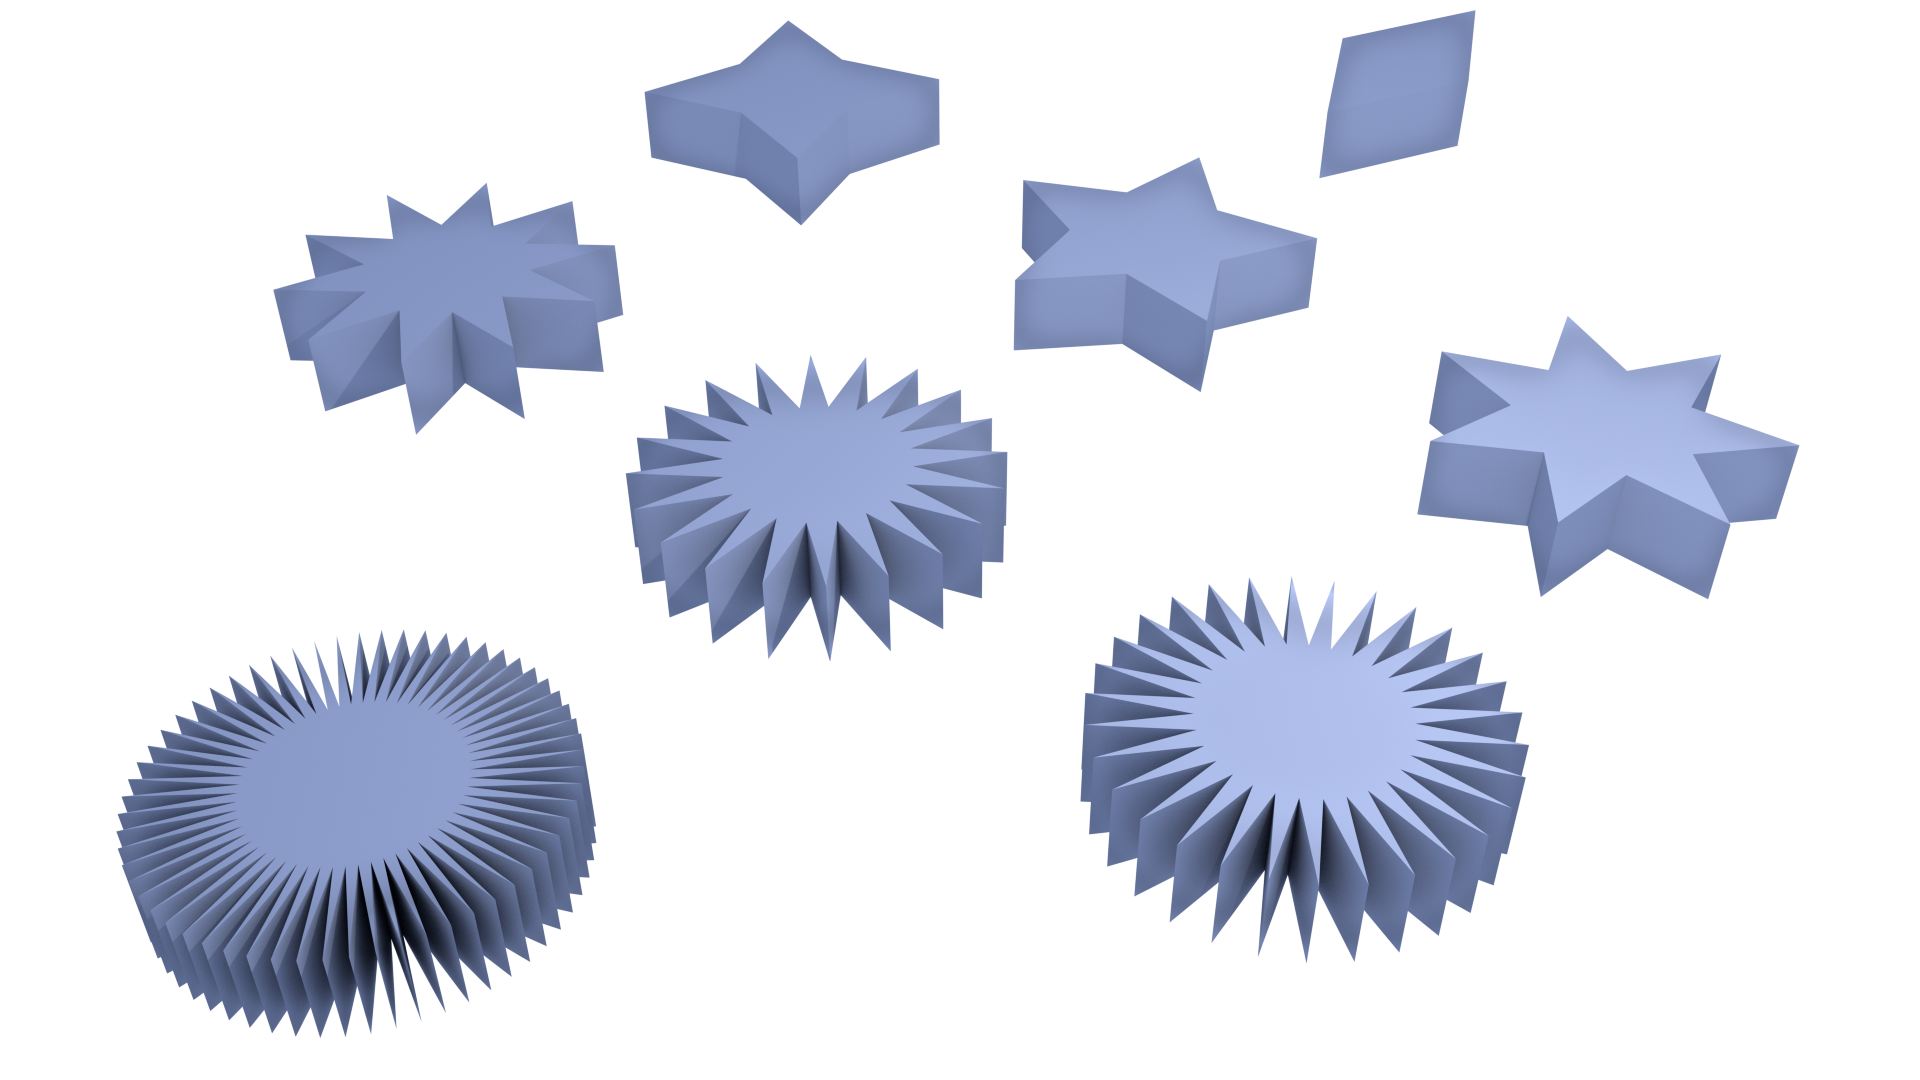
\includegraphics[width=.44\textwidth]{entwurf/star_2-4-5-7-10-20-30-60-trans}}
			{\caption{Gute Unterscheidung von vorn}\label{fig:formen:sterne3d:front-trans}}%
		\end{subfloatrow}
		\hspace*{\columnsep}%
		\begin{subfloatrow}
			\hsize0.7\hsize
			\vbox {%
				\ffigbox[\FBwidth][\FBheight]
				{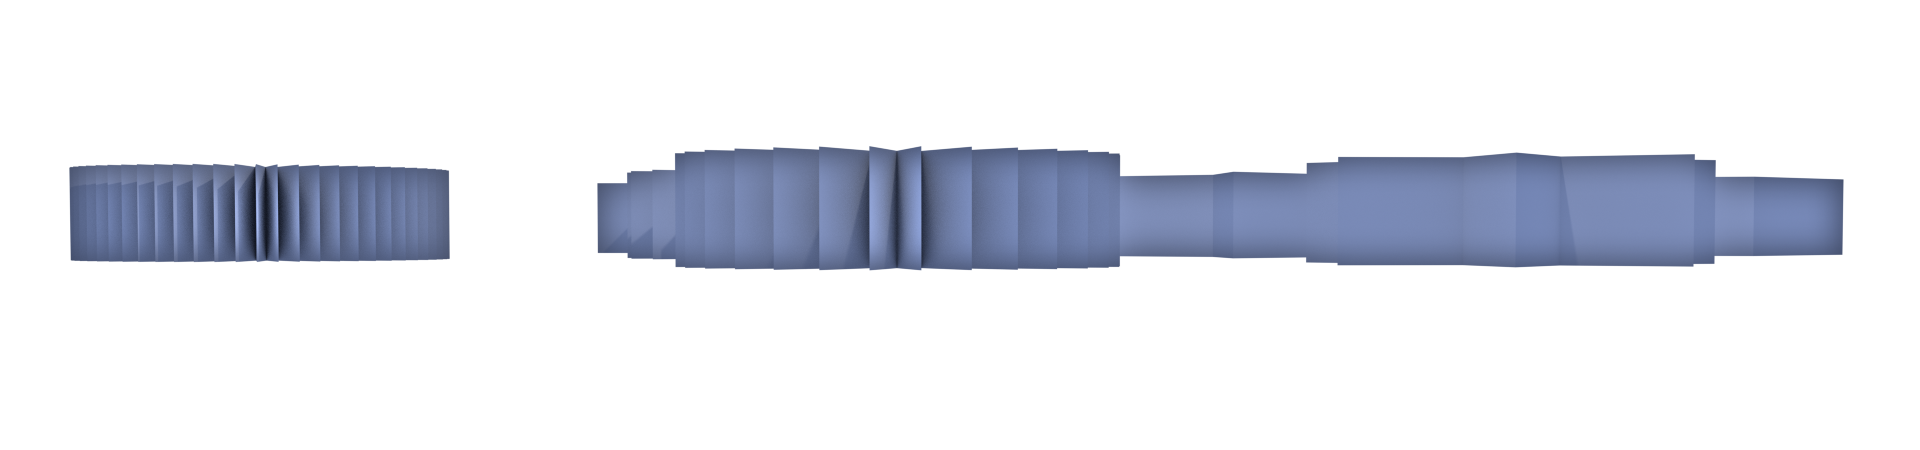
\includegraphics[width=.41\textwidth]{entwurf/star_2-4-5-7-10-20-30-60-seite-trans}}
				{\caption{Die Unterschiede von der Seite \ldots}\label{fig:formen:sterne3d:side-trans}}\vss
				\ffigbox[\FBwidth][\FBheight]
				{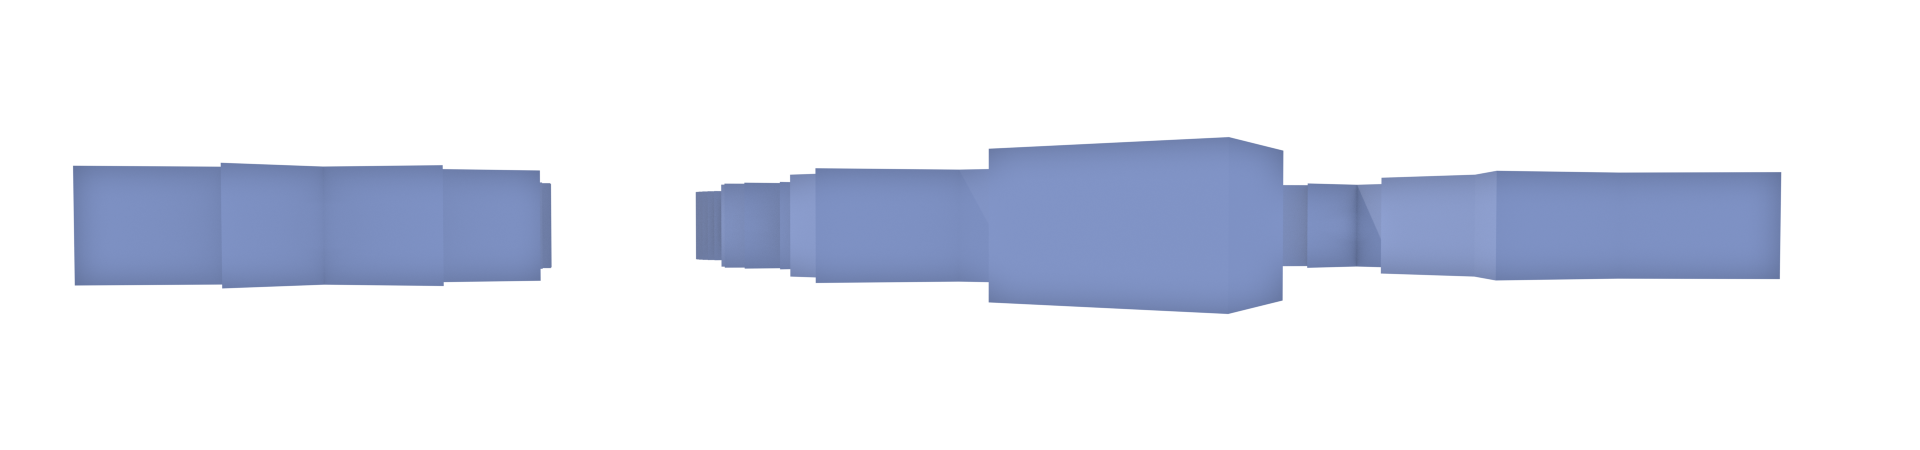
\includegraphics[width=.41\textwidth]{entwurf/star_2-4-5-7-10-20-30-60-oben-trans}}
				{\caption{\ldots bzw. von oben sind kleiner.}\label{fig:formen:sterne3d:top-trans}}
			}
		\end{subfloatrow}
	}
	{\caption{Formgebung mit sternenförmigem, nichtkonvexen Prisma. Erstellt in \tool{Blender}.}\label{fig:formen:sterne3d-trans}}
\end{figure}

Die Anforderung, eine Formgebung zu wählen, die einen ähnlichen Umkugelradius und damit eine einheitliche Größe erhält, einen aus allen Winkeln ähnlichen Durchmesser sowie eine ähnliche Form aufweist, führt zu bestimmten Gruppen von Polyedern. Polyeder sind dreidimensionale Polytope und im engeren Sinne eine Teilmenge des dreidimensionalen Raums, welche ausschließlich durch gerade Flächen begrenzt wird. Darunter zählen unter anderem die fünf \viss{platonischen}{platonischer Körper} \cite{RegularPolyhedra}, die 13 \viss{archimedischen}{archimedischer Körper}, die 13 \viss{catalanischen}{catalanischer Körper} sowie die 92 \vis{Johnson-Körper} \cite{JohnsonPolyeder}. Eine Charakteristik dieser Polyeder ist ihre konvexe Form, was gleichzeitig die Unterscheidung aus der Distanz erschwert. Die prismatischen Polyeder fallen ebenfalls unter diese Kategorie, werden jedoch aus denselben Gründen ausgeschlossen wie die sternenförmigen Prismen.

Andererseits erfüllen die sternförmigen \vis{Kepler-Poinsot-Körper}, auch als »Sternpolyeder« bezeichnet, die Anforderungen. Sie besitzen im Gegensatz zu den vorgenannten Polyedern auch konkave Flächen \cite{KeplerPoinsotSolid} und können daher, wie in der interaktiven Visualisierung von \cite{WebGLUniformPolyhedra} zu sehen, leicht von den konvexen Polyedern unterschieden werden.

Ebenfalls geeignet ist der Vorschlag, eine Sternform durch sogenanntes \textquote{Poken} zu erzeugen: \blockcquote[4]{ProceduralGenerationofSculpturalForms}{By “poke” we mean a function to create a pyramid on each face of a given object. (This is different from Kepler’s stellation operation, which extends the face planes.)}

Somit gibt es mit der auf nichtprismatischen Polyedern basierenden Formgebung eine hohe Anzahl verschiedener Formen, die alle die Anforderung an eine einheitliche Größe, an einen aus allen Blickwinkeln ähnlichen Durchmesser und an die Wiedererkennbarkeit gewährleisten. Lediglich die Unterscheidung innerhalb der konvexen Polyeder kann schwerfallen. Am Deutlichsten unterscheiden sich die \viss{platonischen Körper}{platonischer Körper} untereinander sowie die konvexen von den konkaven, sternförmigen Polyedern.


\section{Strukturereignistaxonomie}\label{sec:strukturereignistaxonomie}
Die ermittelten Ereignisse besitzen Parameter. Die Aufgabe der Visualisierung ist es, diese Parameter für den Nutzer verständlich mit Hilfe der Anwendung von \viss{visuellen Variablen}{visuelle Variable} (siehe \autoref{sec:related:glyphdesign}) aufzubereiten und anzuzeigen. Um die möglichen Kombinationen zu ermitteln, wird eine \vis{Strukturereignistaxonomie} vorgeschlagen.

In dieser werden den Ereignisparametern und \viss{visuellen Variablen}{visuelle Variable} die beiden Variablentypen \vis{Zahlenwert} und \vis{Vokabular} zugeordnet (siehe \autoref{fig:strukturereignistaxonomie:vartype}), die eine Überprüfung der Kompatibilität zwischen Parameter und Variable ermöglichen. Der Typ \vis{Zahlenwert} steht dabei für die Nutzung eines kontinuierlichen Zahlenraumes, während der Variablentyp \vis{Vokabular} eine diskrete, beschränkte Zuordnung mit voneinander disjunkten Elementen beschreibt.

\begin{figure}
	\begin{tikzpicture}[]
	\node {Variablentyen}
	child { node [value] {Zahlenwert} }
	child { node [vocab] {Vokabular} };
	\end{tikzpicture}
	\caption{Variablentypen der \vis{Strukturereignistaxonomie}}\label{fig:strukturereignistaxonomie:vartype}
\end{figure}

Wie in \autoref{tab:ereignis} zu sehen, besitzt ein Ereignis drei Parameter, die jeweils zwischen ein bis drei Freiheitsgraden aufweisen. Die Position hat drei Freiheitsgrade und ist ein \vis{Zahlenwert}, der Zeitpunkt hat einen Freiheitsgrad und ist ebenfalls ein \vis{Zahlenwert}, wohingegen die Ereignisart den Typ \vis{Vokabular} besitzt.

\subsection*{Visuelle Variablen eines Ereigniselements}\label{sec:strukturereignistaxonomie:variablen}
Die \viss{visuellen Variablen}{visuelle Variable} können sowohl als fließender \vis{Zahlenwert} als auch als festes \vis{Vokabular} umgesetzt werden. Für diese Taxonomie werden sieben der elf von Borgo et al. gezeigten, \viss{visuellen Variablen}{visuelle Variable} verwendet (siehe \autoref{sec:related:glyphdesign}). Die Variablen werden teilweise zusammengefasst. So werden Farbwert, Sättigung und Helligkeit als Attribute deklariert und zur neuen, \viss{visuellen Variable}{visuelle Variable} Farbe hinzugefügt. Die Anzahl der Attribute wird analog zu den Ereignisparametern als Freiheitsgrad bezeichnet.

Da Farbwerte bei geringer Sättigung nicht mehr voneinander unterschieden werden können, werden die beiden Attribute, Farbwert und Sättigung, zu einem zusammengefasst. Die Sättigung verbleibt dabei auf ihrem Maximalwert.
%Dadurch kann die Helligkeit leicht als separates Attribut vom Betrachter erkannt werden, wie in \autoref{fig:entwurf:farbtafel} zu sehen.
%\begin{figure}
%	VERGLEICHSBILD MIT WECHSELNDER SÄTTIGUNG UND HELLIGKEIT
%	\includegraphics[width=.8\textwidth]{entwurf/}
%	\caption{Farbtafel mit unterschiedlicher Sättigung und Helligkeit}\label{fig:entwurf:farbtafel}
%\end{figure}

Dadurch ergibt sich die in \autoref{fig:strukturereignistaxonomie} gezeigte Taxonomie. Die Ereignisparameter beziehungsweise \viss{visuellen Variablen}{visuelle Variable} ohne Attribute oder des Typs \vis{Vokabular} besitzen einen Freiheitsgrad von eins.

%\begin{itemize}
%	\item Position: 3 (x, y, z)
%	\item Farbe: 2 (Farbwert/Sättigung, Helligkeit)
%	\item Form: 1, eine Wertzuweisung ist möglich durch die Anzahl der Ecken, Kanten und Flächen. Anderes wie z.B. der Abstand der Ecken vom Körperzentrum kollidiert mit dem Attribut Größe.
%	\item Größe: 1
%	\item Opazität: 1
%\end{itemize}

\begin{figure}
	\ffigbox[\FBwidth] {
		\begin{subfloatrow}
			\ffigbox[\FBwidth] {
				\fbox {
					\begin{tikzpicture}[level 1/.style={sibling distance=1.4cm}]
					\node {Ereignis}
					child { node [value] {Zeitpunkt} }
					child { node {Ort}
						child [verticalChild, first] { node [value] {x} }
						child [verticalChild, second] { node [value] {y} }
						child [verticalChild, third] { node [value] {z} }
					}
					child { node [vocab] {Art}
						child [verticalChild, first] { node {Birth} }
						child [verticalChild, second] { node {Death} }
						child [verticalChild, third] { node {Merge} }
						child [verticalChild, fourth] { node {Split} }
					};
					\end{tikzpicture}
				}
			}
			{\caption{Ereignisparameter sowie Parameterattribute mit zugehörigem Variablentyp.}\label{fig:strukturereignistaxonomie:ereignis}}%
			
			\ffigbox[\FBwidth] {
				\fbox {
					\begin{tikzpicture}[level 1/.style={sibling distance=1.8cm}]
					\node {Visuelle Variable}
					child { node {Position}
						child [verticalChild, first] { node [] {x} }
						child [verticalChild, second] { node [] {y} }
						child [verticalChild, third] { node [] {z} }
					}
					child { node {Farbe}
						child [verticalChild, first] { node [] {Farbwert \& S"attigung} }
						child [verticalChild, second] { node [] {Helligkeit} }
					}
					child { node [] {Gr"oße} }
					child { node [vocab] {Form}	}
					child { node [] {Textur}
						child [verticalChild, first] { node [] {1..*} }
					}
					;
					\end{tikzpicture}
				}
			}
			{\caption{Visuelle Variablen und ihre Attribute. Nicht gekennzeichnete Elemente sind für beide Variablentypen geeignet. Der Asterix steht für eine begrenzte Anzahl an Freiheitsgraden.}\label{fig:strukturereignistaxonomie:variable}}
		\end{subfloatrow}
	}
	{\caption{Schema der \vis{Strukturereignistaxonomie} mit Datenparametern und der visuellen Attribute. Spitze Ecken entsprechen dem Typ \vis{Zahlenwert}, abgerundete dem Typ \vis{Vokabular} (\autoref{fig:strukturereignistaxonomie:vartype}).}\label{fig:strukturereignistaxonomie}}
\end{figure}

Obwohl bei der Form mehrere Freiheitsgrade denkbar wären - etwa eine Kombination aus Anzahl von Ecken mit einem variablen Abstand dieser vom Körperzentrum - wird die Variable auf einen Freiheitsgrad von eins beschränkt. Dies liegt daran, dass der variable Abstand der Ecken mit einer anderen \viss{visuellen Variable}{visuelle Variable} kollidiert, mit der Größe. In der dreidimensionalen Darstellung werden für die Form die in \autoref{sec:grundlagen:3Dformgebung} beschriebenen Polyeder verwendet. Da die Anzahl an Polyedern begrenzt ist und die Unterscheidungsmöglichkeit mit zunehmender Flächenanzahl sinkt, ist die Form nur sehr eingeschränkt als Zahlenwert verwendbar. Dies gilt für die zweidimensionale Darstellung, etwa mittels Polygonen genauso. Daher wird sie in der Taxonomie auf den Typ \vis{Vokabular} beschränkt (siehe \autoref{fig:strukturereignistaxonomie:variable}).

Die Textur ist eine eigenständige, visuelle Variable, auch wenn sie sich mit der Farbe
%, als auch bei der Nutzung als Oberflächenstruktur (Bump oder Displacement Map) mit der Form
überschneidet. Da die Textur jedoch lokale Farbunterschiede innerhalb eines Elements kennzeichnet, kann sie parallel dazu verwendet werden. Sie vereint die in der Arbeit von Borgo et al. genannten \viss{visuellen Variablen}{visuelle Variable} Orientierung, Maserung und Anordnung (siehe \autoref{sec:related:glyphdesign}) und enthält mindestens einen Freiheitsgrad. Dieser kann jedoch durch die lokale Bestimmung weit höher liegen, etwa wenn verschiedene Bereiche der Textur für unterschiedliche Datenparameter verwendet werden.

Der Freiheitsgrad einer \viss{visuellen Variable}{visuelle Variable} gibt die Anzahl der Datenparameter an, die ihr zugewiesen werden kann. Umgekehrt zeigt der Freiheitsgrad eines Datenparameters die Anzahl der benötigten \viss{visuellen Variablen}{visuelle Variable}.

Bei der Bestimmung der Attribute wurde darauf geachtet, ein umfassendes Spektrum der Gestaltgesetze nutzen zu können (siehe \autoref{sec:grundlagen:gestaltgesetze}). Alle \viss{visuellen Variablen}{visuelle Variable} fallen unter den Einfluss des \viss{Gesetzes der Prägnanz}{Gesetz der Prägnanz}. Mit der Position kann das \vis{Gesetz der Nähe} sowie das \vis{Gesetz der gemeinsamen Region} genutzt werden, eine Kombination der Position mit den anderen \viss{visuellen Variablen}{visuelle Variable} resultiert in der Verwendbarkeit des \viss{Gesetzes der Kontinuität}{Gesetz der Kontinuität}. Bis auf die Position kann mit allen visuellen Attributen das \vis{Gesetz der Ähnlichkeit} genutzt werden. Das \vis{Gesetz der Geschlossenheit} kann mit der Position angewendet werden, falls durch entsprechende Zuweisung die Elemente nah beieinander lägen und sie eine geschlossene Form bilden. Mit den hier definierten Variablen können somit sechs Gestaltgesetze genutzt werden.

Die Opazität wird aufgrund des Ziels der überlagerten Darstellung von \vis{Ereignisobjekt} und \vis{Partikelobjekt} in der Taxonomie trotz Vorteilen bei überlagerter Darstellung innerhalb eines Objekts (siehe \autoref{sec:glyphprototyp:opazitaet}) ausgeklammert. Sie würde die Sichtbarkeit der Glyphen im Vergleich zur Partikeldarstellung oder des Hintergrundes zu sehr einschränken.

Animationen bieten weitere visuelle Variablen wie Bewegungsrichtung, Bewegungsbahn, Beschleunigung und Geschwindigkeit als auch die Veränderung der anderen Attribute und eröffnen damit die Nutzung des \viss{Gesetzes der Gleichzeitigkeit}{Gesetz der Gleichzeitigkeit} sowie des \viss{Gesetzes der gemeinsamen Bewegung}{Gesetz der gemeinsamen Bewegung}. Sie werden im Rahmen dieser Arbeit jedoch nicht behandelt.

Die \viss{visuellen Variablen}{visuelle Variable} lassen sich durch den Betrachter unterschiedlich gut unterscheiden.
%In der folgenden Sortierung nach ihrer Unterscheidungsgüte stehen die am Leichtesten zu unterscheidenden Attribute ganz oben. (QUELLE)
%\begin{enumerate}
%	\item Position
%	\item Farbwert
%	\item Größe
%	\item Form
%	\item Helligkeit
%	\item Opazität
%\end{enumerate}
Solche mit höherer Unterscheidungsgüte sollten bevorzugt gewählt werden. Form, Helligkeit und Textur besitzen eine geringere Güte. Daher sind sie besser zur Verwendung mit dem Typ \vis{Vokabular} geeignet, denn die Anzahl der Varianten ist im Vergleich zu einer kontinuierlichen (unendlichen) Menge an Varianten, wie es beim Typ \vis{Zahlenwert} der Fall ist, gering. Bei einem \vis{Vokabular} können die Varianten einer \viss{visuellen Variable}{visuelle Variable} weit auseinanderliegen, was die Unterscheidungsmöglichkeit verbessert.

\subsection*{Problem der lokalen und temporalen Häufung}\label{sec:strukturereignistaxonomie:haeufung}
Die Anzahl der Ereignisse, die denselben Ort oder denselben Zeitpunkt aufweisen können, ist unbekannt. Schon eine geringe Anzahl identischer Orte oder Zeitpunkte kann je nach Zuordnung der \viss{visuellen Variablen}{visuelle Variable} zu einer überlagerten, nicht mehr unterscheidbaren Darstellung der Ereignisglyphen führen.

Daher sollte eine \vis{visuelle Variable} reserviert werden, um eine solche Anhäufung von Ereignissen anzuzeigen und programmatisch zu behandeln. Formal ausgedrückt bedeutet diese Reservierung das Hinzufügen der Häufung zu den Datenparametern der \vis{Strukturereignistaxonomie}.

Bei der Visualisierung der Häufung kann die intuitive Wirkung der visuellen Attribute genutzt werden. So würde groß, opaque und dunkel eine starke Häufung symbolisieren und klein, transparent und hell hingegen eine niedrige.

\subsection*{Zuweisung der visuellen Variablen}\label{sec:strukturereignistaxonomie:zuweisung}

Aufgrund der Zielstellung der Arbeit, die Strukturereignisse im Raum der Partikel anzuzeigen, wird die Position dem Ortsparameter des Ereignisses als \vis{visuelle Variable} zugewiesen. Darüber hinaus wird jedem Ereignisparameter nur ein visuelles Attribut zugeordnet, um eine Verminderung der präattentiven Wahrnehmung durch Mehrfachzuweisungen zu vermeiden (siehe \autoref{sec:related-praattentiveWirkung}).

Weiterhin werden die Anzahl an Freiheitsgraden sowie die Kompatibilität der Variablentypen berücksichtigt und die Häufung als Parameter aufgenommen, so dass sich die in \autoref{tab:strukturereignistaxonomie:zuweisung} aufgeführte Zuweisungsmatrix ergibt. Der Ereignisart stehen durch ihren Typ als \vis{Vokabular} die meisten \viss{visuellen Variablen}{visuelle Variable} zur Verfügung. Zu beachten ist, dass die Farbe und die Textur gleichzeitig mehrere Parameter visualisieren können.
%Die Zuweisungsmöglichkeiten betragen weniger als 36, da nicht zwei Parameter dieselbe visuelle Variable besitzen dürfen.

\begin{table}
	\begin{tabularx}{\textwidth}{@{}LL|CCCC@{}}
		\toprule
		Parameter / Variable &  & Zeitpunkt & Ereignisort & Ereignisart & Häufung \tabularnewline
		& Freiheitsgrad & 1 & 3 & 1 & 1 \tabularnewline
		\midrule
		Position & 3 & \kreuz (vergeben) & fest & \kreuz (vergeben) & \kreuz (vergeben) \tabularnewline
		Größe & 1 & \checkmark & \kreuz & \checkmark & \checkmark \tabularnewline
		Farbe & 2 & \checkmark & \kreuz & \checkmark & \checkmark \tabularnewline
		Form & 1 & \kreuz (Typ) & \kreuz & \checkmark & \kreuz (Typ) \tabularnewline
		Textur & $+$ & \checkmark & \kreuz (vergeben) & \checkmark & \checkmark \tabularnewline
		\bottomrule
	\end{tabularx}
	\caption{Zuweisungsmatrix der \viss{visuellen Variablen}{visuelle Variable} zu den Ereignisparametern. Berücksichtigt werden ausreichender Freiheitsgrad, Variablentyp (Typ) sowie Regeln (fest, vergeben). $+$ steht für das Intervall $[1,\infty)$.}
	\label{tab:strukturereignistaxonomie:zuweisung}
\end{table}


\subsection*{Glyphprototyp}
Zur Überprüfung der Zuweisung von Datenparametern zu den \viss{visuellen Variablen}{visuelle Variable} dienen Mockups. Aufgrund der Vielzahl der in \autoref{sec:strukturereignistaxonomie:zuweisung} genannten Kombinationsmöglichkeiten wird eine programmatische Erstellung der Mockups gewählt, deren Funktionsweise in \autoref{sec:glyphprototyp} dargelegt ist.


\section{Gestaltung der Glyphen}\label{sec:visualisierung:glyphen}
\blockcquote[64]{infantidou2001evidentials}{[...] so that the first acceptable interpretation to occur to the hearer is the one [the speaker] intended to convey.}

Die \vis{Ereignisglyphen}{Ereignisglyph} sind die Schnittstelle zwischen den berechneten Ereignisdaten und dem Anwender. Die \vis{Strukturereignistaxonomie} und der zugehörige \vis{Glyphprototyp} wurden vor allem als Hilfestellung zu ihrer Gestaltung entwickelt.

%TODO Fertigstellen
%TODO Thesen hier formulieren!
UNFERTIG

\subsection*{Dimension der Glyphdarstellung}\label{sec:visualisierung:glyphen3d}
Auswertung des Prototypen:

- Polygone nicht so gut geeignet, da Unterscheidung auf Entfernung schwer möglich und auch hier noch Abhängigkeit vom Blickwinkel

- daher zweidimensionale, vordefinierte Bilder an Eventtypen gekoppelt, 

Um eine präattentive Wirkung zu erzielen (siehe \autoref{sec:related-praattentiveWirkung}), wird jeder Ereignisparameter nur mit jeweils einer \viss{visuellen Variable}{visuelle Variable} verknüpft.


\subsection*{Form und Abgeschlossenheit}
Es wird eine annähernd rechteckige Form verwendet, um einen Kontrast zur runden Gestalt der kugelförmigen Partikelvisualisierung zu schaffen. Falls der innere Bereich des Glyphs dem Nutzer keinen Anhaltspunkt für die Orientierung geben kann, wird die Unterkante als eine stumpfe, nach unten zulaufende Spitze gestaltet (siehe \autoref{fig:visualisierung:glyph-art}). Ihre auffällige Wirkung wird bei der Positionierung der Glyphen (siehe \autoref{sec:vis:glyph-pos}) genutzt.

Weiterhin wird die Außenkante des Glyphs mit einem Rahmen versehen, um das \vis{Gesetz der Geschlossenheit} zu berücksichtigen und dabei im Inneren Platz für die Visualisierung der Ereignisart und -zeit zu erhalten. Dieser Rand wird nicht zu dünn gestaltet, um Aliasing an hochfrequenten (schmalen, nah beieinanderliegenden) Kanten und das damit verbundene Flimmern während der Anzeige zu verringern.

\subsection*{Kodierung der Ereignisart}

\begin{figure}
	\ffigbox[\FBwidth] {
		\begin{subfloatrow}
			\vbox {%
				\ffigbox[\FBwidth][\FBheight]
				{
					
\includegraphics[width=.2\textwidth]{vis/GlyphEventTypeAbstractBirthWhite}
					
\includegraphics[width=.2\textwidth]{vis/GlyphEventTypeAbstractDeathWhite}
					
\includegraphics[width=.2\textwidth]{vis/GlyphEventTypeAbstractMergeWhite}
					
\includegraphics[width=.2\textwidth]{vis/GlyphEventTypeAbstractSplitWhite}
				}
				{\caption{Abstrakt symbolische Darstellungsvariante}\label{fig:visualisierung:glyph-art:abstrakt}}\vss
				\ffigbox[\FBwidth][\FBheight]
				{
					
\includegraphics[width=.2\textwidth]{vis/GlyphEventTypeBirthWhite}
					
\includegraphics[width=.2\textwidth]{vis/GlyphEventTypeDeathWhite}
					
\includegraphics[width=.2\textwidth]{vis/GlyphEventTypeMergeWhite}
					
\includegraphics[width=.2\textwidth]{vis/GlyphEventTypeSplitWhite}
				}
				{\caption{Erzählerisch symbolische Darstellungsvariante}\label{fig:visualisierung:glyph-art:erzaehl}}
			}
		\end{subfloatrow}
	}
	{\caption{Kodierung aller vier Ereignisarten mit zwei unterschiedlichen, symbolischen Darstellungsvarianten. Von links nach rechts sind Glyphen für Birth, Death, Merge und Split abgebildet. Außerdem ist die Glyphform sichtbar.}\label{fig:visualisierung:glyph-art}}
\end{figure}

Es werden zwei symbolische Darstellungsvarianten (siehe \autoref{sec:related:glyphdesign}) entworfen. Die abstrakte Variante hat keinen Bezug zum Inhalt, wogegen die erzählerische Variante eine Konnektivität zu den Begriffen der Strukturereignisse beinhaltet. So steht bei der zweiten Variante der Asterisk für Geburt, ein Kreuz für den Tod sowie eine umschließende als auch eine nach außen geöffnete Klammer für Verschmelzung beziehungsweise Trennung (siehe \autoref{fig:visualisierung:glyph-art:erzaehl}). Ein Ziel der für die Auswertung entwickelten Umfrage stellt die Prüfung da, ob beide Varianten eine intuitive Deutung zulassen und ob eine der beiden leichter interpretiert werden kann. %Siehe Evaluation.

Die Kodierungsvarianten könnten mit den in \autoref{tab:glyphprototyp:ereignisart} vorgeschlagenen Werten für Farbwert und Helligkeit erweitert werden. Allerdings werden beide Farbattribute für die Kodierung der Zeit reserviert und eine Doppelbelegung für die Ereignisart wird vermieden. Denn die \vis{Strukturereignistaxonomie} fordert eine eindeutige Zuweisung der visuellen Attribute, so dass bei einer Doppelbelegung eine automatische Änderung der Zuweisung des jeweils anderen Parameters erfolgen muss. Solch eine automatische Änderung wird im \vis{Glyphprototyp} unterstützt und sie führt bei der Bedienung zu Verwirrung. Daher wird bei der Implementation des \tool{MegaMol}-Plugins darauf verzichtet.

\subsection*{Kodierung der Ereigniszeit}\label{sec:vis:glyh-zeit}
Die Visualisierung der Zeit wird unter Verwendung von Farbwert, Helligkeit oder Textur durchgeführt. Scheinbar ist die Textur zusammen mit der Ereignisart doppelt belegt, jedoch unterstützt diese \vis{visuelle Variable} mehrere Freiheitsgrade (siehe \autoref{sec:strukturereignistaxonomie:variablen}). Gemäß der \vis{Strukturereignistaxonomie} wird die Sättigung unveränderbar auf den Maximalwert eingestellt.
%sowieso nicht mehr in der Taxonomie Die Opazität wird nicht verwendet, um nicht die Sichtbarkeit im Vergleich zur Partikeldarstellung oder des Hintergrundes einzuschränken.

Alle drei \viss{visuellen Variablen}{visuelle Variable} ermöglichen einen uneingeschränkten Einsatz des Typs \vis{Zahlenwert}, was für die Darstellung der Zeit von Vorteil ist.
%TODO Bilder

%TODO THESEN Füllung, Helligkeit, Form - mit Eva verknüpfen


\section{Renderer und Shader}\label{sec:renderer}

%TODO Fertigstellen!
UNFERTIG

immer zur Kamera ausgerichtet vgl. Sprites

Shader:
common.btf für Standardlicht
billboard.btf für Billboards in OGL 2.1
Nutzung von \tool{OpenGL} 2.1 zur Wahrung der Kompatibilität mit den MM Modulen.
Laden der Bilder mit lodepng

Nutzung der glm Bibliothek, da dadurch die Datentypen in C++ und in GLSL konsistent angelegt werden können.

Die Texturen haben einen festgelegten Pfad im Ordner der ausführenden Datei, da der Nutzer sie nicht ändern können soll. Dies liegt darin begründet, dass der \vis{Billboard}-Shader zur Darstellung des Zeitpunktes eines Ereignisses auf bestimmte Farben in der Textur angewiesen ist. So wird die Farbe lila (rgb 255, 0, 255) abhängig von den Einstellungen der Zeitkodierung dynamisch ersetzt. Bei der Auswahl der Zeitkodierung als Farbe oder Helligkeit wird durch den Shader ein heller Grauton in die lilagefärbten Bereiche geschrieben und alle anderen Pixel der Textur werden mit einer von der Zeit abhängigen Farbe ersetzt, bei der Auswahl als Textur wird der Bereich abhängig von der Zeit mit Dunkel- oder Hellgrau überschrieben und die anderen Bereiche der Textur bleiben unangetastet (siehe \autoref{sec:berechnungen:glyph}).


\subsection*{Positionierung der Glyphen}\label{sec:vis:glyph-pos}

Durch die in der Aufgabenstellung formulierte Bedingung, die Daten der Partikel als auch die Daten der Strukturereignisse im selben Raum zu visualisieren, wird die überlagernde Darstellung angewandt (siehe \autoref{sec:related-visAnordnung}) und die Position der \viss{Ereignisglyphen}{Ereignisglyph} wird an die Positionen der entsprechenden Strukturveränderungen im Partikeldatensatz gesetzt. Dazu wird der Ort des \CFDterms{Wurzelpartikels}{Wurzelpartikel} eines betroffenen Clusters verwendet. Die Positionen des oder der \SECterm{Partnercluster} sind dabei nicht relevant, was bei großen Clustern zu Problemen der Lokalisierung des Ereignisses führen könnte. Eine Implementation, die in Abhängigkeit der Parameter der \SECterm{Ereignisheuristik} sowie der \CFDterm{Clustergröße} der betroffenen (Partner-)Cluster eine gewichtete Positionierung entlang der Verbindungslinie zwischen den \CFDterms{Wurzelpartikeln}{Wurzelpartikel} vornimmt, wäre für eine Weiterentwicklung wünschenswert.

Im Verhältnis zur Position des Ereigniselements wird der \vis{Ereignisglyph} genau oberhalb platziert. Aufgrund der in \autoref{sec:visualisierung:glyphen} beschriebenen äußeren Form wird angenommen, dass der Nutzer das Ereignis intuitiv unterhalb des Glyphen einordnet.


\subsection*{Parameterslots} 
Parameterslots bieten dem Nutzer die Möglichkeit, während der Laufzeit des Programms Parameter ändern zu können.

Um dem in \autoref{sec:strukturereignistaxonomie:haeufung} beschriebenen Problem der lokalen und temporalen Häufung zu begegnen, wird unter Berücksichtigung der in \autoref{tab:strukturereignistaxonomie:zuweisung} aufgeführten Zuweisungsmöglichkeiten ein änderbarer Parameter für die Glyphgröße bereitgestellt. Somit wird der Häufung die Größe als visuelles Attribut zugewiesen. Weiterhin unterstützt die veränderbare Glyphgröße den Wechsel zwischen der Makro- und Mikrosicht, indem der Parameter je nach Benutzerpräferenzen bei der Makrosicht große und bei der Mikrosicht kleine Werte annehmen kann.

%TODO Zuweisungen Art, Zeit
Ein zweiter Parameterslot wurde zur benutzerdefinierte Kontrolle über die Visualisierung der Zeit mit einer der drei in \autoref{sec:vis:glyh-zeit} vorgestellten Varianten implementiert. Auch gibt es einen dritten und vierten Slot für die Ereignisposition sowie die -art. Zwar bieten diese beiden nur jeweils eine Auswahlmöglichkeit, jedoch ist das \MMStruktur{StaticRenderer Modul} durch diese Art der Behandlung leicht erweiterbar.



\subsection*{Parallelisierung der Anzeigeberechnungen}
Bei der Zuweisung der \viss{visuellen Variablen}{visuelle Variable} zu den Ereignisparametern sind Berechnungen notwendig. Diese bewirken, dass die Anzeige bei einer hohen Anzahl von Ereignissen verzögert erfolgt, etwa nach Änderungen von Parametern des \MMStrukturs{StaticRenderer Moduls}{StaticRenderer Modul}. Da die Berechnungen für jedes Ereignis unabhängig voneinander erfolgen, können sie parallel ausgeführt werden. Aufgrund des Zugriffs auf die Quelldaten über das Inkrementieren von Zeigern, muss eine Einteilung der Berechnungen in eine feste Anzahl von Threads geschehen, deren Ermittlung mit der C++11 Standardbibliothek \wichtig{thread} erfolgt. Eine andere Möglichkeit wäre gewesen, diese Berechnungen in den Geometrieshader der Grafikkarte zu verlegen.

\section{Visualisierung der Cluster}\label{sec:visualisierung:cluster}
Die \tool{MegaMol} Molekularsimulation der Partikel nutzt entweder nur die Position als \vis{visuelle Variable} oder zusätzlich die Farbe. Beide werden zur Visualisierung der Cluster verwendet.

Um die Qualität der Clusterberechnung zu untersuchen und dem Nutzer Vergleichsmöglichkeiten mit den Ereignissen an die Hand zu geben, wird allen Partikeln desselben Clusters dieselbe Farbe zugeordnet. Im ersten berechneten Zeitschritt erfolgt diese Farbzuweisung für jeden Cluster zufällig oder anhand von Eigenschaften des \CFDterms{Wurzelpartikels}{Wurzelpartikel} (siehe \autoref{sec:fast-depth}), in den darauffolgenden Zeitschritten wird die Farbe desjenigen Partnerclusters des vorhergehenden Zeitschrittes übernommen, der die meisten gemeinsamen Partikel aufweist. Sollte der Cluster keinen \SECterm{Partnercluster} besitzen, wird eine neue zufällige Farbe zugewiesen.

Weiterhin wird eine zufällige Färbung für jeden Zeitschritt implementiert, die als alternative Darstellungsform gewählt werden kann.

\section{Darstellung des Zeitverlaufs}
Durch eine ähnliche Bewegungsrichtung und Geschwindigkeit sowie durch örtliche Nähe der Partikel lassen sich Zusammenhangskomponenten während der Animation erkennen. Dies nutzt die Clustereinfärbung mittels einer Farbvererbung, so dass die Wanderung von Cluster verfolgt werden kann.

Das \MMStruktur{StaticRenderer Modul} bietet eine statische, gleichzeitige Anzeige der \viss{Ereignisglyphen}{Ereignisglyph} für alle Zeitschritte bzw. für die folgenden oder vorhergehenden Zeitschritte im Vergleich zum aktuelle gewähltem. Um das Entstehen der Strukturereignisse besser zu verfolgen, wird auch ein dynamisches Einblenden während der Animation ermöglicht. Unterstützt werden diese Varianten durch die visuelle Kodierung der Glyphen (\autoref{sec:visualisierung:glyphen}).




\chapter{Evaluation}

Die Berechnungen werden auf einem dedizierten Rechner, unabhängig vom Entwicklungssystem durchgeführt (siehe zweites System in \autoref{sec:hardware}) und für verschiedene Parametereinstellungen durchgeführt. Die für die Entwicklung und Auswertung notwendigen Berechnungen erstreckten sich aufgrund der in \autoref{sec:eva:ressourcen} gezeigten Berechnungsdauer über mehrere Wochen. Einzelheiten zum Aufbau der dafür benötigten Module sind in \autoref{sec:pluginaufbau} zu finden.

Die Berechnungen werden sowohl qualitativ als auch quantitativ bewertet und die Thesen der Visualisierung werden durch eine Umfrage sowohl unter Experten von Molekularsimulationen als auch unter Laien geprüft. Auch fließt ein Teil der Umfrage bei der Beurteilung des Ereignisverlaufes ein. Erklärungen in der \href{http://www.instant.ly/s/wY5Ax}{Umfrage} wurden nur sparsam eingesetzt, um die Benutzer unvoreingenommen urteilen zu lassen und zu prüfen, ob die Visualisierung auch ohne Hintergrundwissen Rückschlüsse zulässt.

Die Erfassung quantitativer Daten war nicht Teil der Aufgabenstellung, wurde jedoch während der Entwicklung erforderlich aufgrund des experimentellen Charakters einer Heuristik und der Überprüfung der Funktionalität der beiden entwickelten \CFD und \SECC Algorithmen. Eine Analyse dieser Daten ergänzt die qualitative Betrachtung.

\section{Clusterbildung}\label{sec:eva:cluster}

\begin{figure}
	\ffigbox[\FBwidth] {
		\begin{subfloatrow}
			\hsize0.7\hsize
			\vbox {%
				\ffigbox[\FBwidth][\FBheight]
				{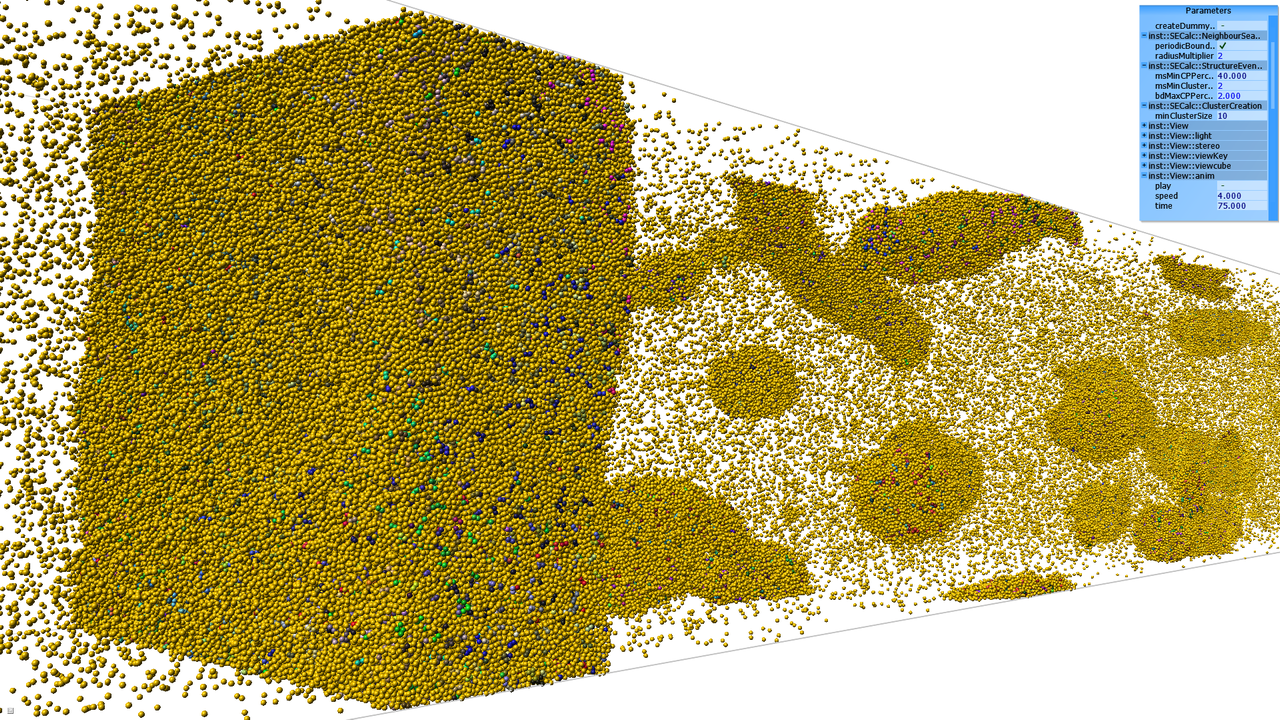
\includegraphics[width=.41\textwidth]{eva/2R-01-f75-Block-small}}
				{\caption{Zweifacher Radius.}\label{fig:eva:cluster-2r}}\vss
				\ffigbox[\FBwidth][\FBheight]
				{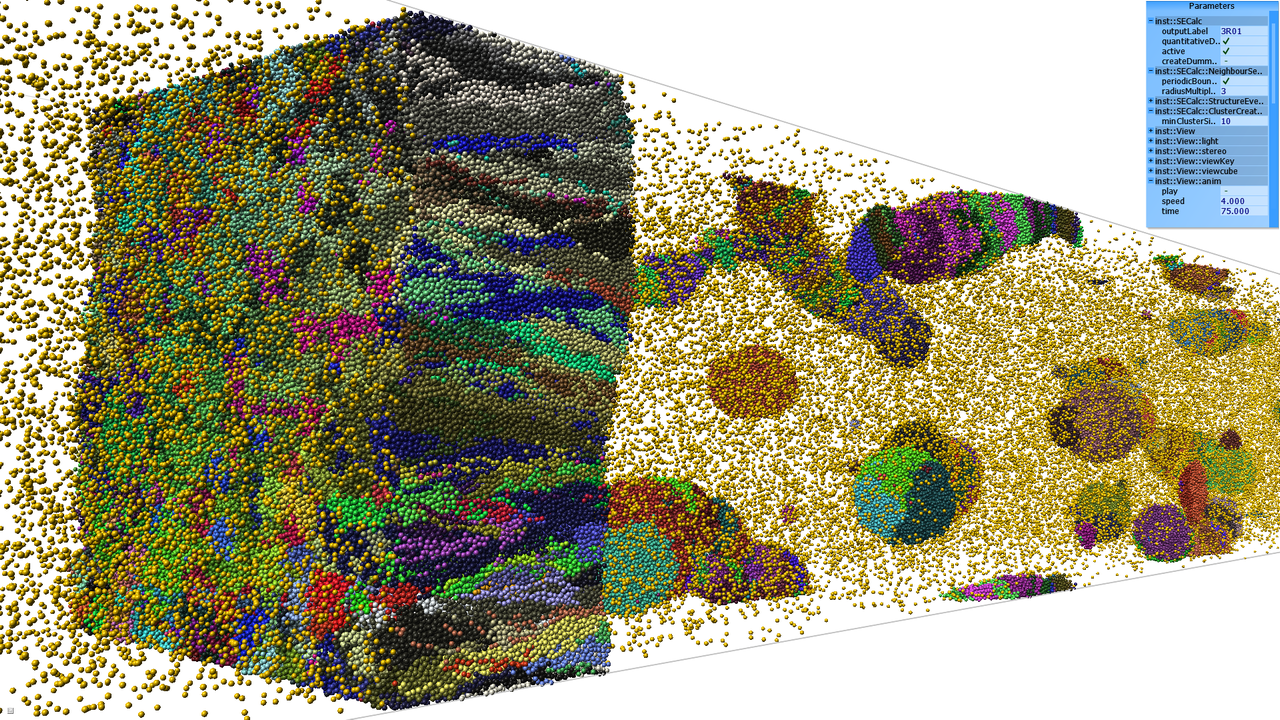
\includegraphics[width=.41\textwidth]{eva/3R-01-f75-Block-small}}
				{\caption{Dreifacher Radius.}\label{fig:eva:cluster-3r}}\vss
				\ffigbox[\FBwidth][\FBheight]
				{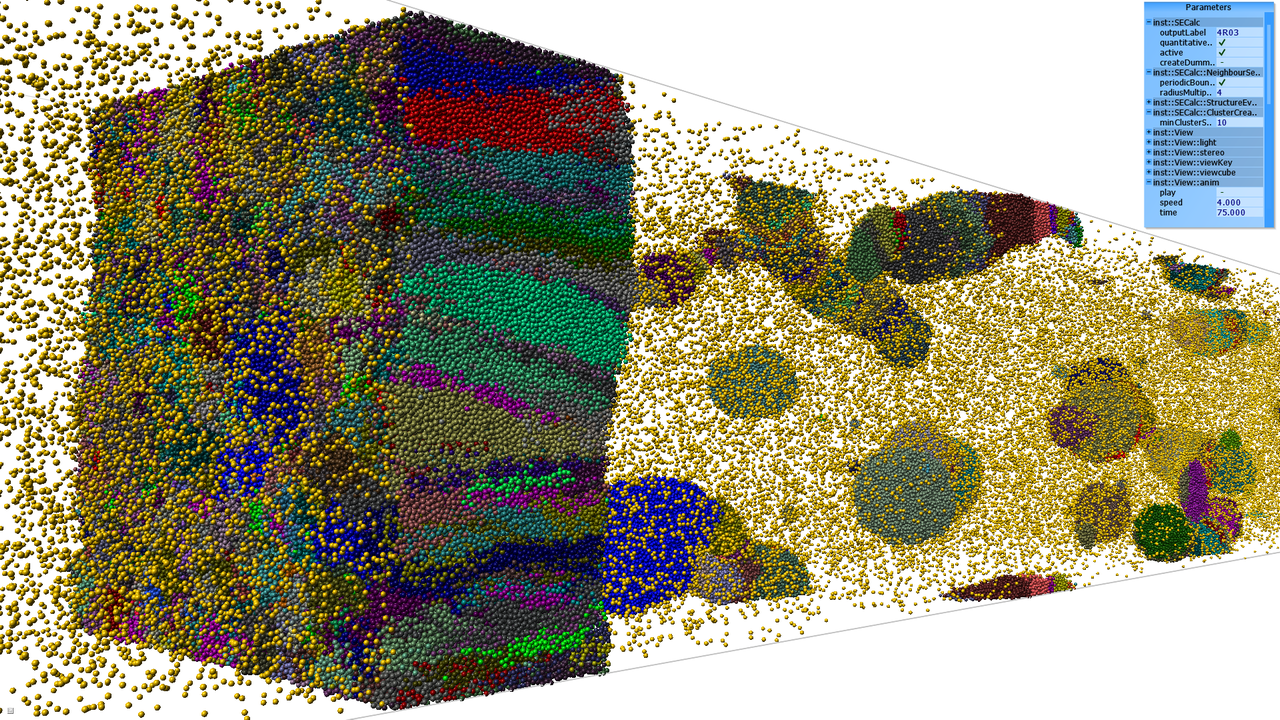
\includegraphics[width=.41\textwidth]{eva/4R-03-f75-Block-small}}
				{\caption{Vierfacher Radius.}\label{fig:eva:cluster-4r}}
			}
		\end{subfloatrow}
		\hspace*{\columnsep}%
		\begin{subfloatrow}
			\hsize0.7\hsize
			\vbox {%
				\ffigbox[\FBwidth][\FBheight]
				{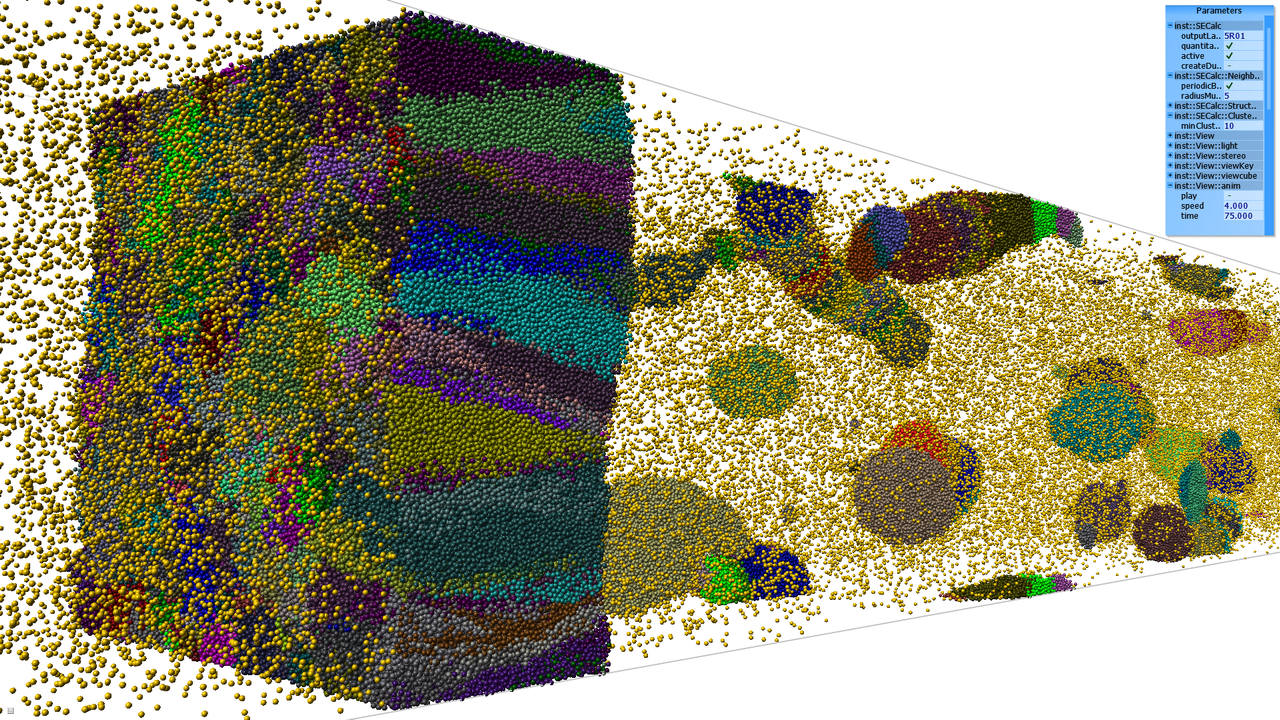
\includegraphics[width=.41\textwidth]{eva/5R-01-f75-Block-small}}
				{\caption{Fünffacher Radius.}\label{fig:eva:cluster-5r}}
				\ffigbox[\FBwidth][\FBheight]
				{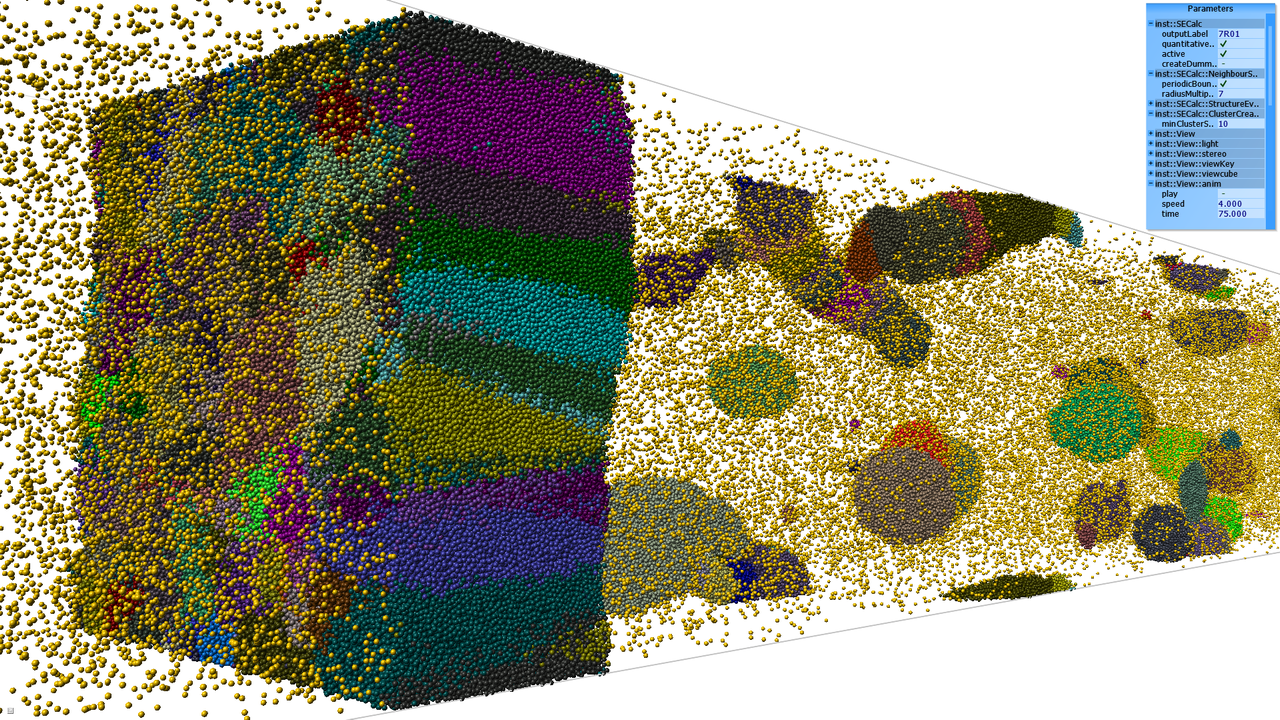
\includegraphics[width=.41\textwidth]{eva/7R-01-f75-Block-small}}
				{\caption{Siebenfacher Radius.}\label{fig:eva:cluster-7r}}\vss
				\ffigbox[\FBwidth][\FBheight]
				{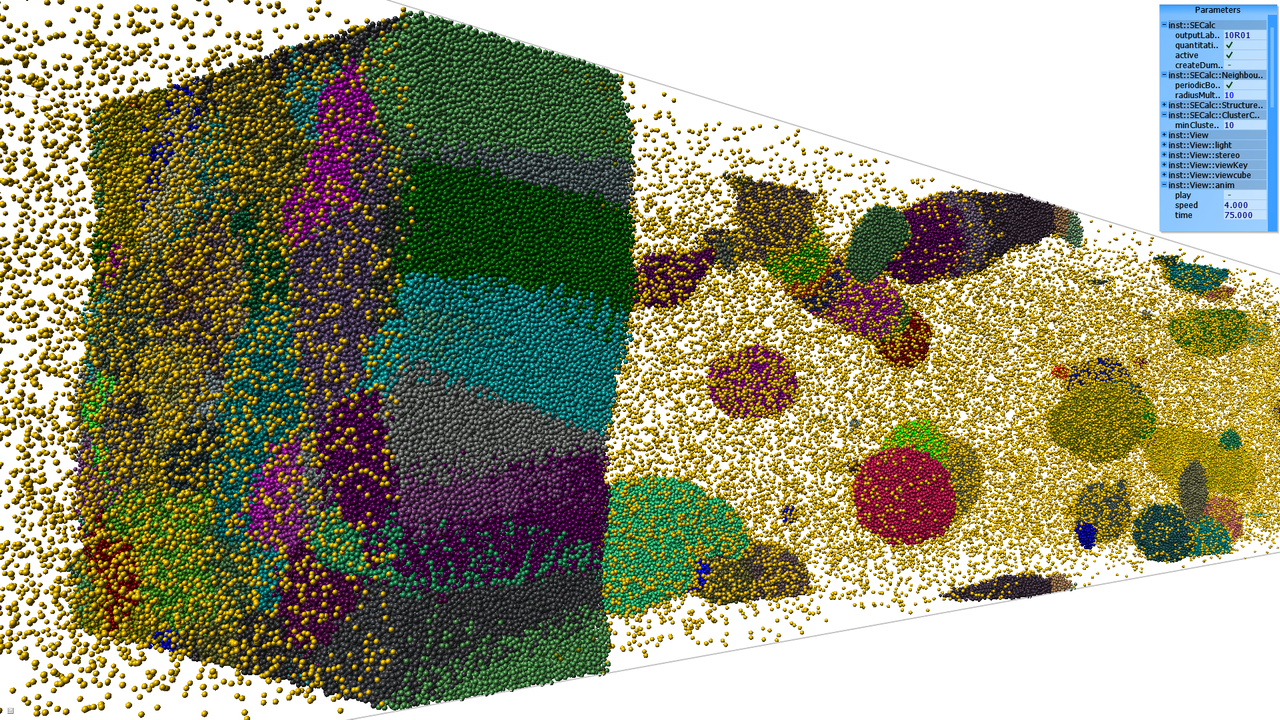
\includegraphics[width=.41\textwidth]{eva/10R-01-f75-Block-small}}
				{\caption{Zehnfacher Radius.}\label{fig:eva:cluster-10r}}
			}
		\end{subfloatrow}
	}
	{\caption{Clusterbildung abhängig von der Reichweite bei der Nachbarschaftserkennung. Dabei ist das Vielfache des Partikelradius angegeben. Die Aufnahmen sind bei Zeitschritt 75 entstanden.}\label{fig:eva:cluster}}
\end{figure}

\begin{figure}
	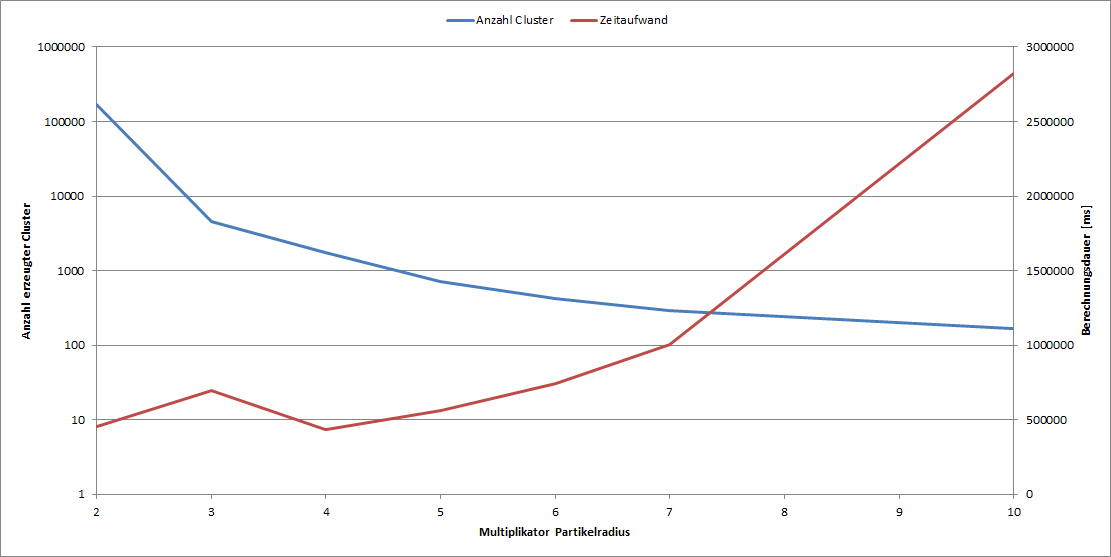
\includegraphics[width=1\textwidth]{eva/cluster-r-alle}
	\caption{Logarithmische Anzahl der erzeugten Cluster sowie die Berechnungszeit in Abhängigkeit des Radius der Nachbarschaftssuche bei Zeitschritt 75.}\label{fig:eva:cluster-r-alle}
\end{figure}

In \autoref{fig:eva:cluster} ist deutlich zu sehen, dass bei zweifachem Partikelradius bei der Nachbarschaftserkennung nur sehr kleine Cluster gefunden werden. Dies liegt daran, dass bei dieser geringen Suchreichweite kaum Nachbarn vorhanden sind. Somit ist diese Radiuseinstellung zu klein, auch ist die Clusteranzahl mit zwei Größenordnungen über der Anzahl bei dreifachem Radius viel zu hoch (siehe \autoref{fig:eva:cluster-r-alle}). Bei fünffachen Radius beträgt die Anzahl der gefunden Cluster bei Zeitschritt 75 mit 722 Clustern nur noch 40\% der Anzahl mit vierfachem Radius. Der Zeitaufwand liegt mit etwa 500 Sekunden nur 30\% höher, was ein guter Kompromiss ist. So wird der fünffache Radius als Basiseinstellung für die Berechnung über den gesamten Simulationszeitraum verwendet und als ergänzende Daten der sieben- und der zehnfache Radius ebenfalls betrachtet.

\begin{figure}
	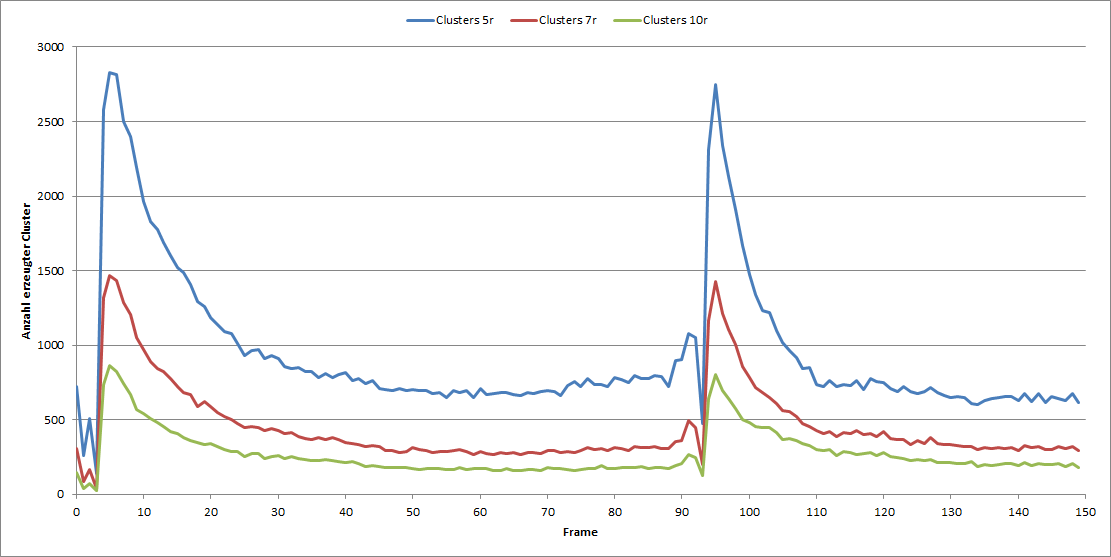
\includegraphics[width=1\textwidth]{eva/cluster-r}
	\caption{Anzahl der erzeugten Cluster in Abhängigkeit des \CFDterm{Partikelradiusmultiplikator} der Nachbarschaftssuche über alle Zeitschritte.}\label{fig:eva:cluster-r}
\end{figure}

Der große Einfluss des gewählten Radiusmodifikator bei der Nachbarschaftssuche ist in \autoref{fig:eva:cluster-r} auch über den gesamten Simulationszeitraum sichtbar. Mit zunehmenden Suchradius nimmt die Anzahl an Cluster stark ab. Je größer die Suchreichweite, desto höher ist die Anzahl der Nachbarn pro Partikel und auch Partikel, die etwas weiter entfernt sind, werden zu Nachbarn. Damit verringert sich effektiv die Anzahl an lokalen Maxima, denn wenn bei kleinerem Suchradius, wie dem fünffachen Partikelradius, zwei lokale Maxima nebeneinanderliegen, so werden diese bei größeren Suchradien während des \SECC zu einem zusammengefasst, da die beiden Maxima dann selbst direkte Nachbarn sind und so das tiefere, höhere Maximum das kleinere verdrängt.

Weiterhin ist der große Einfluss der durch den Simulationsverlauf bedingten Strukturänderungen auf die Clusteranzahl zu erkennen. Dies ist durch die veränderte Topologie und damit der variierenden Anzahl an lokalen Maxima bedingt. Die Auswirkungen werden bei der Ereignisanalyse in \autoref{sec:eva:ereignis-verlauf} genannt.

\section{Quantitative Analyse der Ereignisermittlung}\label{eva:quantitativ}

Bei der Erkennung von Birth und Death Ereignissen wurde eine zusätzliche Erkennungsmöglichkeit über die Anteile an gemeinsamen Partikeln implementiert (siehe Parameter in \autoref{sec:ereigniserkennung}). Die Überprüfung der Birth- und Deathereignisse mit Anteilen von 0-5\% an gemeinsamen Partikeln ergab einen über alle Anteile identischen Wert (siehe digitale Logs des \gls{dse}). Das bestätigt die Stabilität der gewählten Birth bzw. Death Erkennung über Cluster ohne Partner und auf diesen Paramenter braucht daher nicht weiter eingegangen zu werden.

\begin{figure}
	\ffigbox[\FBwidth] {
		\begin{subfloatrow}
			\vbox {%
				\ffigbox[\FBwidth][\FBheight]
				{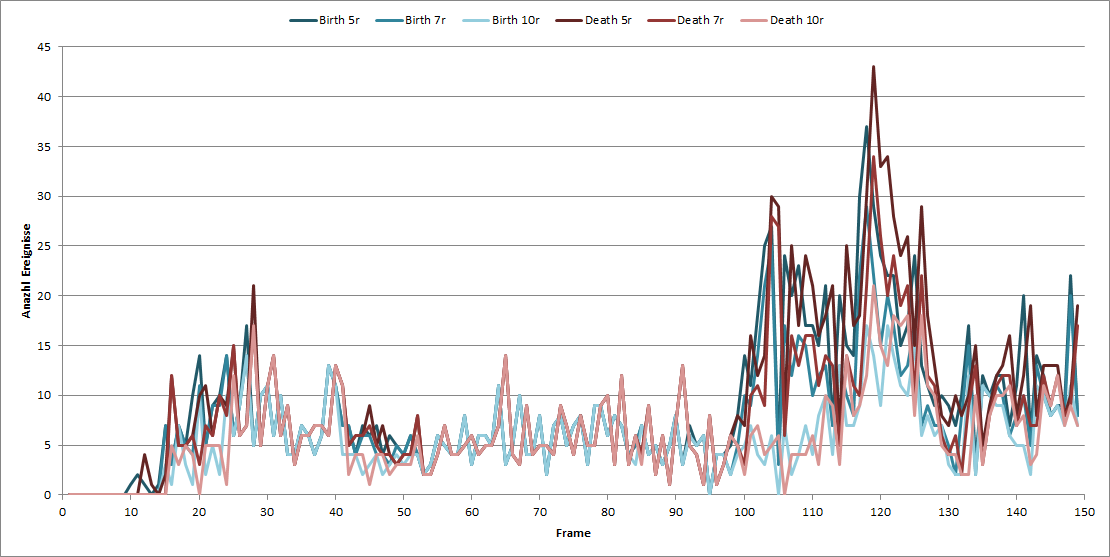
\includegraphics[width=1\textwidth]{eva/birth-death-r}}
				{\caption{Birth (blau) und Death (rot)}\label{fig:eva:birth-death-r}}\vss
				\ffigbox[\FBwidth][\FBheight]
				{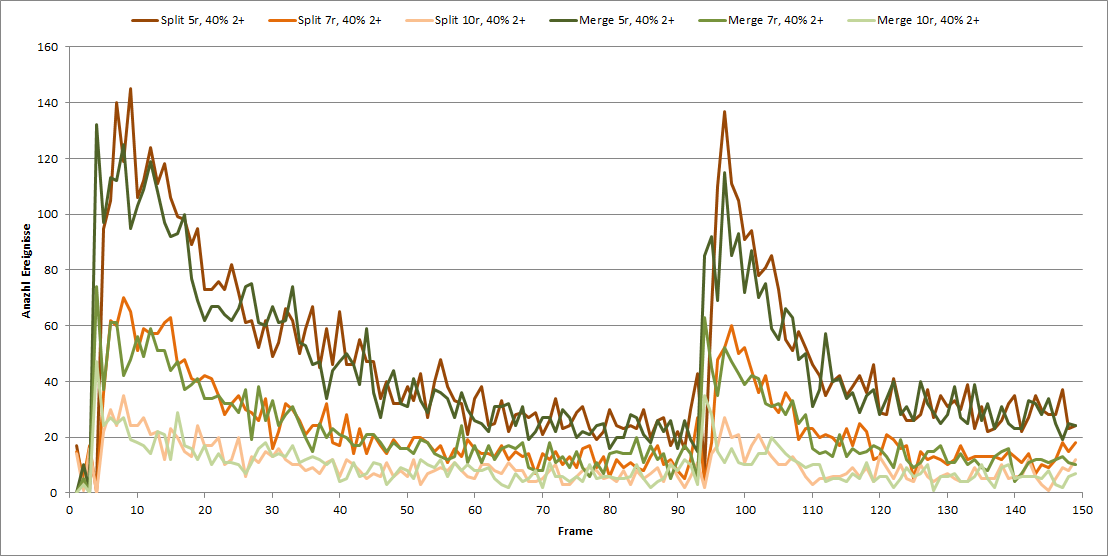
\includegraphics[width=1\textwidth]{eva/merge-split-r}}
				{\caption{Merge (grün) und Split (orange) bei einer Einstellung von zwei \SECterms{Partnerclustern}{Partnercluster} mit jeweils 40\% gemeinsamen Partikeln}\label{fig:eva:merge-split-r}}
			}
		\end{subfloatrow}
	}
	{\caption{Anzahl der Ereignisse über den Zeitraum der Simulation in Abhängigkeit des Radius der Nachbarschaftssuche}\label{fig:eva:ereignis-r}}
\end{figure}

\subsection*{Abhängigkeit von der Nachbarschaftssuche}
In \autoref{fig:eva:ereignis-r} ist zu sehen, dass Birth und Death weit weniger von der Radiuseinstellung bei der Nachbarschaftssuche abhängen als Merge und Split. Das kommt daher, weil diese Ereignisse vor allem bei kleinen Tröpfchenstrukturen vorkommen, bei denen die Anzahl von Clustern aufgrund der geringen Partikelanzahl unabhängig der Radiuseinstellung ist.

Merge und Split hingegen zeigen eine starke Abnahme ihrer Anzahl mit zunehmendem Radius (Helligkeit in \autoref{fig:eva:merge-split-r}). Dies hängt mit der geringeren Clusteranzahl und der damit verbundenen, kleineren \SECterm{Clustervergleichsmatrix} zusammen, wodurch bei denselben Ereigniserkennungsparametern weniger Ereignisse erkannt werden können.

\subsection*{Abhängigkeit vom Simulationsverlauf}\label{sec:eva:ereignis-verlauf}
Die Anzahl der Ereignisse ändert sich in Abhängigkeit vom Simulationsverlauf stark (siehe \autoref{sec:simulation}). Dies korreliert mit der Anzahl der Cluster (siehe \autoref{fig:eva:cluster-r}) und fällt insbesondere bei der Trennung und das Zusammenstoßen der Flüssigkeitsfronten ins Auge. Auf Merge und Split hat dieses Geschehnis einen großen und unmittelbaren Einfluss, auf Birth und Death einen kleineren.
Daraus kann abgeleitet werden, dass viele Merge- und Splitereignisse innerhalb der Fronten stattfinden, während Birth und Death eher bei Tröpfchen vorkommen. Weiterhin nehmen Merge und Split ab, je länger die Trennung bzw. der Zusammenstoß zurückliegen. Bei Zeitschritt 90 ist ihre Anzahl auf ein Fünftel im Vergleich zum Beginn der Frontentrennung zusammengeschrumpft. Dieses Verhältnis gilt für einen fünffachen Radius bei der Ermittlung der Nachbarn. Je höher dieser Suchradius gewählt wird, desto geringer sind die Differenzen bei der Anzahl der Strukturereignisse, da auch die Gesamtzahl der Ereignisse abnimmt.

Die Merge- und Splitereignisse weisen eine ähnliche Anzahl bei der Trennung und beim Zusammenstoß auf. Die Birth- und Deathereignisse ebenfalls. Als Besonderheit nehmen diese Ereignisse nach dem Zusammenstoß nicht ab, sondern stark zu. Das könnte daran liegen, dass sich viele sehr kleine Cluster bilden oder Phänomene wie der »Nulltiefenwert \CFDterm{Einpartikelcluster}« auftreten (siehe \autoref{sec:eva:ereignisse-quali-verlauf}, \autoref{sec:nulltiefenwert-einpartikel-cluster}). In \autoref{sec:eva:ressourcen} wird die Annahme über die Bildung kleiner Clustern untermauert.

\subsection*{Abhängigkeit von den Ereignisparametern}\label{sec:eva:ereignis-param}
Die durch den Nutzer einstellbaren Parameter für die Ereigniserkennung sind die Anzahl an \SECterms{Partnerclustern}{Partnercluster} und die Anteile an gemeinsamen Partikeln dieser Cluster. Birth und Death werden mit einer festen Anzahl von null Partnern erkannt, besitzen aber einen einstellbaren Anteil von gemeinsamen Partikeln. Wie am Anfang dieses Kapitels beschrieben, hat dieser keinen Einfluss auf die Ereignisanzahl bei relevanten, geringen Werten. Somit werden nur die Merge- und Splitereignisse betrachtet.

Die in \autoref{fig:eva:split-param} abgebildeten Verläufe zeigen mit strikteren Parametereinstellung einen erwarteten Abfall der Ereignisanzahl. Insbesondere die Erhöhung der Mindestanzahl an benötigten \SECterms{Partnerclustern}{Partnercluster} schlägt sich enorm nieder. Drei \SECterm{Partnercluster} mit jeweils 30\% gemeinsamen Partikeln treten fast nie auf, eine Senkung auf 25\% bewirkt eine im Vergleich deutliche Erhöhung, liegt jedoch gerade einmal auf ähnlichem Niveau wie zwei Partnern mit 45\% gemeinsamen Partikel. Eine mögliche Einstellung mit mindestens vier benötigten Partnern wird daher einen wesentlich geringeren Anteil erfordern, um mit der Heuristik Merge- und Splitereignisse erkennen zu lassen.

Trotz dieser Unterschiede ist die Verteilung der Ereignisanzahl über den Simulationsverlauf hinweg für alle Parametereinstellungen ähnlich. Insbesondere zeigt auch die Einstellung mit drei Mindestpartnern und 25\% Anteil ähnliche Ausschläge wie die Verläufe mit deren zwei, so zum Beispiel bei den Zeitschritten 95 und 97.

\begin{figure}
	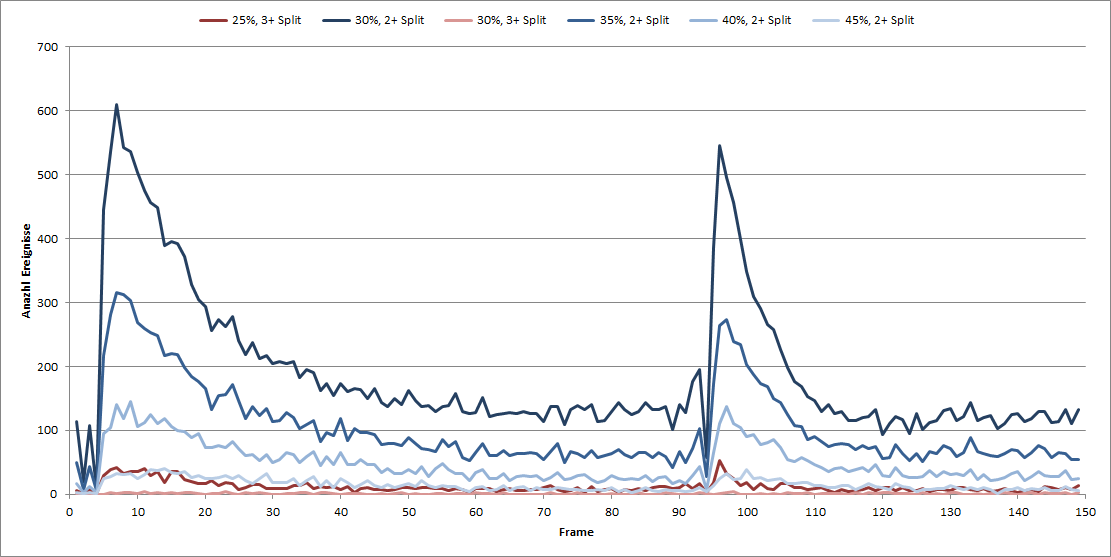
\includegraphics[width=1\textwidth]{eva/split-param}
	\caption{Anzahl der Ereignisse in Abhängigkeit der Parameter. Rote Verläufe sind Messungen für drei \SECterm{Partnercluster}, blaue Verläufe für zwei. Für Merge sind Verlauf und Verhältnisse analog. Die Prozentangaben stehen für die Anteile gemeinsamer Partikel pro Partner.}\label{fig:eva:split-param}
\end{figure}

In der folgenden, qualitativen Analyse werden Möglichkeiten und Grenzen der Algorithmen aufgezeigt.

\section{Qualitative Analyse der Ereignisermittlung}\label{sec:eva:ereignisse}
%TODO Gespeicherte Daten anschauen, einige Durchschnittsbilder und v.a. kritische Punkte/Grenzen herauspicken

Aufgrund des Mangels eines optimalen Systems kann keine Bestimmung der Güte der bei der Ereigniserkennung zum Einsatz kommenden Heuristik getroffen werden. Allerdings ermöglicht die überlagerte Visualisierung des Partikel- und des \viss{Ereignisobjektes}{Ereignisobjekt} (siehe \autoref{sec:renderer}) eine Bewertung der Ereignisermittlung durch einen Vergleich mit den Positionen von Clustern. Durch eine ähnliche Bewegungsrichtung und Geschwindigkeit der Partikel sowie durch ihre örtliche Nähe oder Ferne lassen sich Agglomerationen von Partikeln während der Animation erkennen. Unterstützt wird dies durch die Einfärbung der Partikel nach ihrer Clusterzugehörigkeit. Dies hilft auch, ohne der Zuhilfenahme von \viss{Ereignisglyphen}{Ereignisglyph} eine Verschmelzung oder Trennung über mehrere Zeitschritte hinweg zu erkennen, so dass in einigen Fällen eine Beurteilung über die korrekte Ermittlung der Ereignisart getroffen werden kann. Zu diesen Fällen zählt das Trennen oder Verschmelzen von Filamenten oder von Tröpfchen.

\subsection*{Ereignisse im Simulationsverlauf}\label{sec:eva:ereignisse-quali-verlauf}

\begin{figure}
	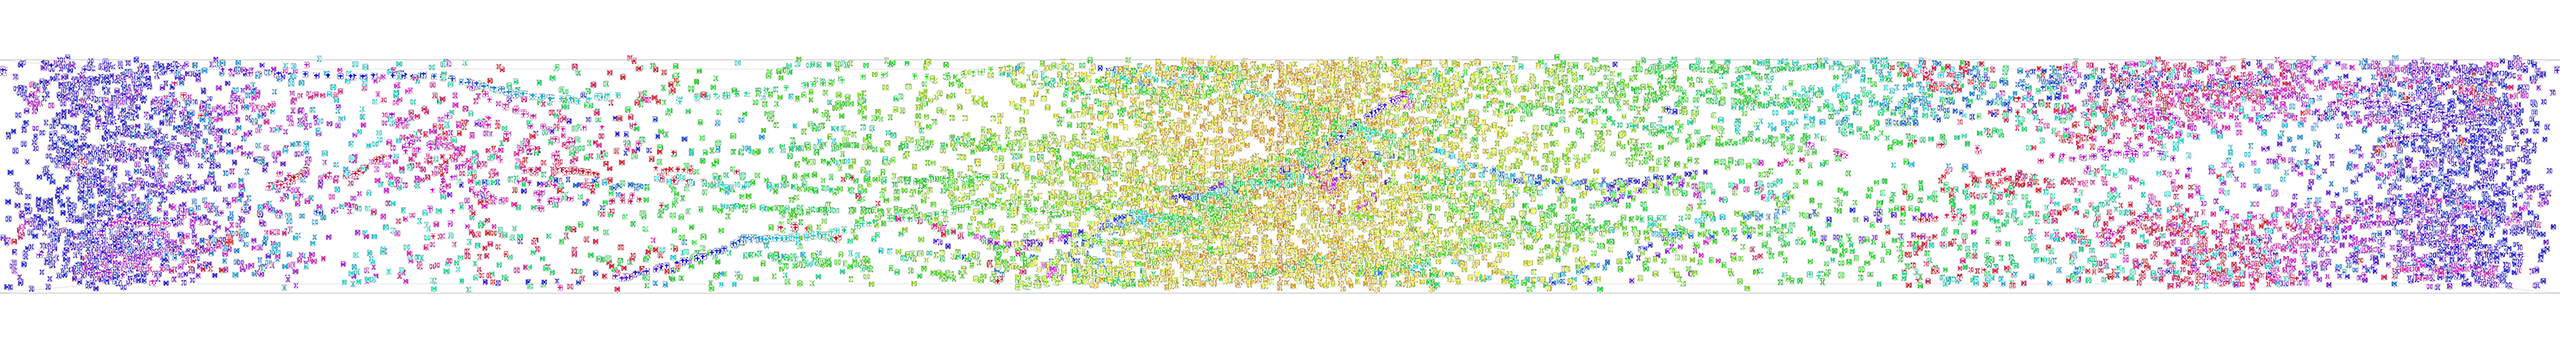
\includegraphics[width=1\textwidth]{eva/EventFlow-Hue-5r-10-ms2-40-bd2-cropped-small}
	\caption{Alle Ereignisse visualisiert im Simulationsraum. Die Zeit ist über den Farbwert der Glyphen visualisiert. Die Glyphgröße beträgt 0,012. Der \CFDterm{Partikelradiusmultiplikator} beträgt fünf, die \SECterm{Ereignisheuristik} arbeitet mit zwei \SECterms{Partnerclustern}{Partnercluster} mit jeweils 40\% Anteil an gemeinsamen Partikeln.}\label{fig:eva:EventFlow-Hue-5r-10-ms2-40-bd2-cropped-small}
\end{figure}

In \autoref{fig:eva:EventFlow-Hue-5r-10-ms2-40-bd2-cropped-small} sind alle Ereignisse bei einem \CFDterm{Partikelradiusmultiplikator} von fünf visualisiert. Die Zeit der Ereignisses ist mit der Farbe kodiert. Vor allem im zweiten und vierten Fünftel sind deutlich horizontal langgestreckte, perlenkettenartige Verläufe der \viss{Ereignisglyphen}{Ereignisglyph} zu sehen. Ihre Anordnung zeigt, dass durch die Bewegung der Flüssigkeit nach außen entstehen Filamentstrukturen die meisten der Strukturereignisse verursacht werden. Auch werden Ereignisse durch die Tröpfchen oder die Flüssigkeitsfronten erzeugt, jedoch ist die Zahl der durch die Tröpfchen verursachten Ereignisse geringer und die durch die Fronten sind über die kurzen Achsen des Simulationsraumes verteilter. Dies kann nur während des Auftauchens der Glyphen während der Animation beurteilt werden, was dieses \href{https://www.youtube.com/watch?v=0K7J3ISMrDM}{Video der Animation mit zufälliger Clustereinfärbung} zeigt.

Diese Eigenschaft der Berechnung wurde ebenfalls in der Umfrage behandelt, um zu überprüfen, ob die Visualisierung korrekte Rückschlüsse ziehen lässt. Dabei ist vor allem die Expertenbeurteilung von Belang. Aufgrund der kleinen Anzahl werden in \autoref{fig:eva:umfrage-letzte} auch die Antworten der Laien aufgeführt.

\begin{figure}
	\ffigbox[\FBwidth] {
		\begin{subfloatrow}
			\vbox {%
				\ffigbox[\FBwidth][\FBheight]
				{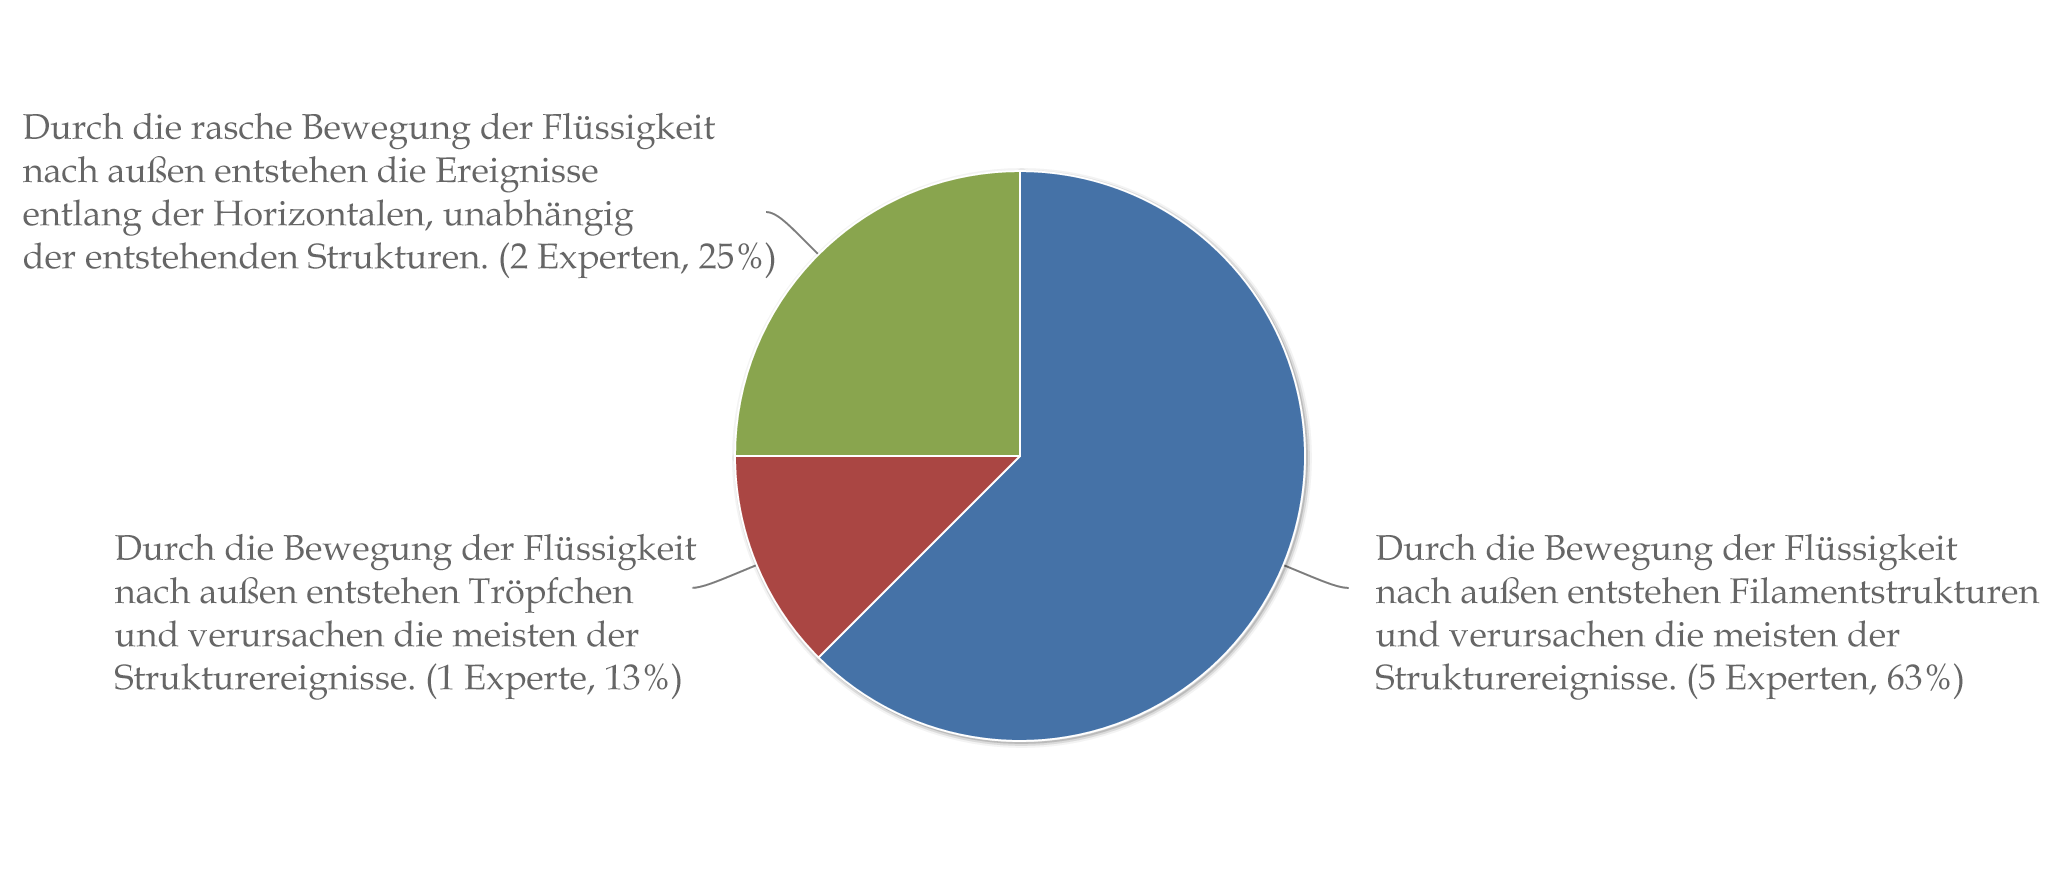
\includegraphics[width=1\textwidth]{eva/umfrage-letzte-experten}}
				{\caption{Antwortverteilung von acht Experten}\label{fig:eva:umfrage-letzte-experten}}\vss
				\ffigbox[\FBwidth][\FBheight]
				{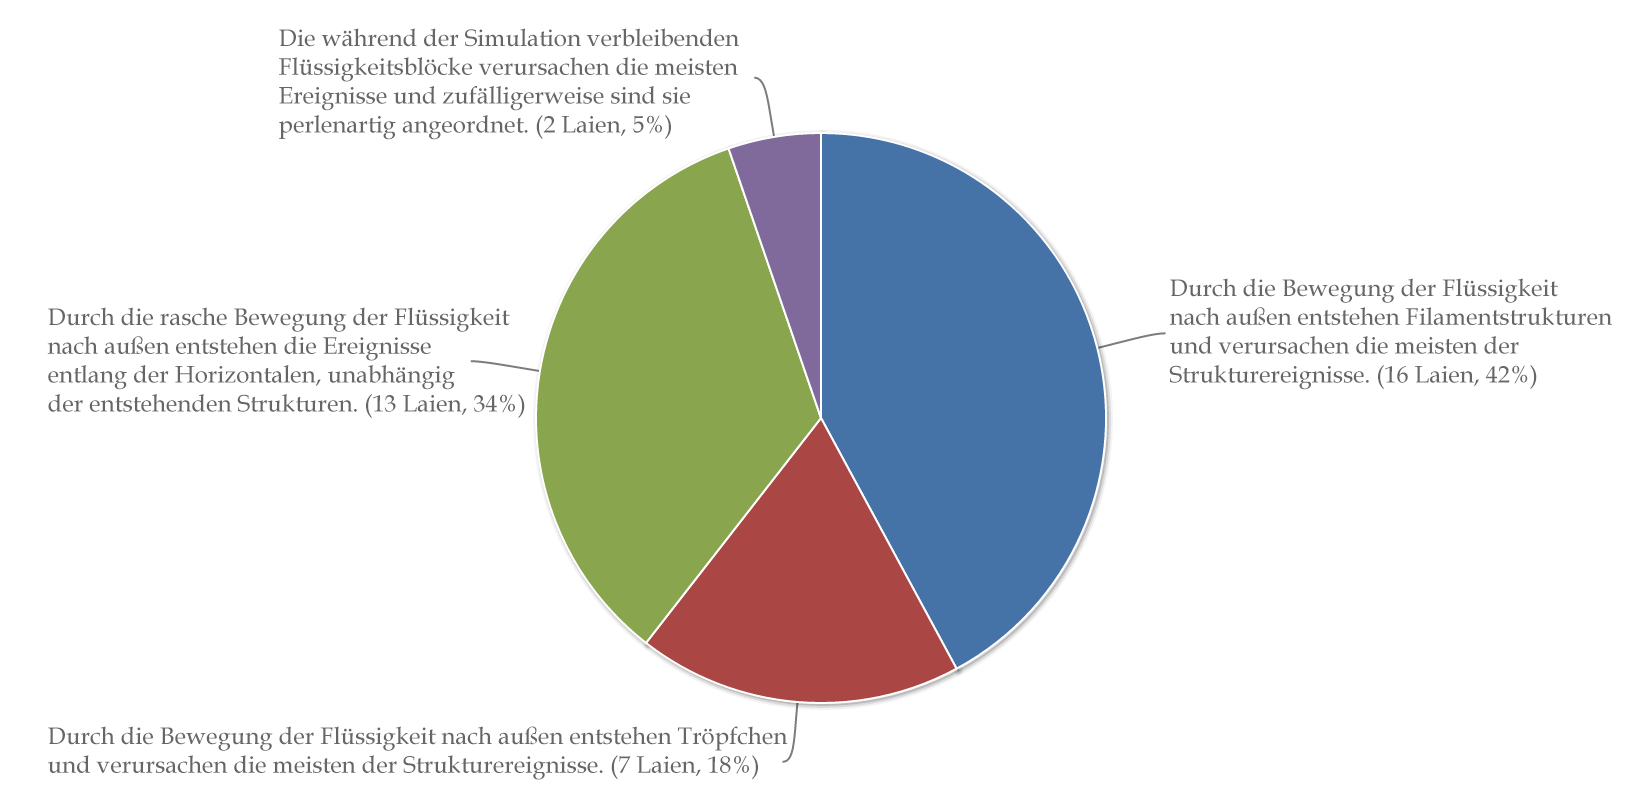
\includegraphics[width=1\textwidth]{eva/umfrage-letzte-laien}}
				{\caption{Antwortverteilung von 38 Laien}\label{fig:eva:umfrage-letzte-laien}}
			}
		\end{subfloatrow}
	}
	{\caption{Inhaltliche Beurteilung der Ereignisvisualisierung nach Vergleich eines Videos der Simulation mit der statischen Visualisierung aller Ereignisse analog zu \autoref{fig:eva:EventFlow-Hue-5r-10-ms2-40-bd2-cropped-small}}\label{fig:eva:umfrage-letzte}}
\end{figure}

Vier Antwortmöglichkeiten wurden gegeben. Durch die Bewegung der Flüssigkeit nach außen entstehen (a) Filamentstrukturen und verursachen die meisten der Strukturereignisse oder (b) Tröpfchen und verursachen die meisten der Strukturereignisse oder (c) die Ereignisse entlang der Horizontalen, unabhängig der entstehenden Strukturen erzeugen die meisten Strukturereignisse oder (d) die während der Simulation verbleibenden Flüssigkeitsblöcke verursachen die meisten Ereignisse und zufälligerweise sind sie perlenartig angeordnet. Insgesamt 46\% der Teilnehmer beantworteten die Frage korrekt mit (a), von den Experten waren es mit 63\% bedeutend mehr.

Überraschend war, dass selbst zwei der Experten die Ereignisse unabhängig der Strukturen einordneten (Antwort c), was im Sinne der Ereignisvisualisierung falsch ist. Dies deutet die Schwierigkeit an, die Visualisierung ohne Erklärungen zu interpretieren. Das mit 34\% weit mehr Laien diese Antwort gewählt haben zeigt, dass die Beurteilung ohne Hintergrundwissen noch schwieriger fällt.

Die zahlreichen, innerhalb der beiden Flüssigkeitsfronten entstehenden Strukturereignisse lassen sich visuell nur schwer beurteilen. Ihre Entstehung kann jedoch mit der Abhängigkeit des \CFD von lokalen Maxima (siehe \autoref{sec:eva:cluster}) und damit verbundenen Schwankung der Clusterzugehörigkeit von Partikeln begründet werden, wodurch die \SECterm{Ereignisheuristik} viele Ereignisse erkennt. Durch einen Schnitt im Simulationsraum kann ... TODO SCREENSHOT
%TODO Bild mit Clipplane interpretieren

Diese Art von Ereignissen innerhalb von Strukturen ohne deren sichtbare Trennung oder Vereinigung werden als \SECterm{Ereignisrauschen} bezeichnet. Es muss vom in \autoref{sec:ereigniserkennung} erwähnten Rauschen abgegrenzt werden, da es nicht die Bildung kleiner \SECterm{Partnercluster} beschreibt.

Birth- und Deathereignisse treten sehr gehäuft an kleinen Clustern auf. Interessanterweise bilden sie bei der Visualisierung über den gesamten Zeitverlauf mehrere, wie in \autoref{fig:eva:birth-death-flow} abgebildeten Ketten.

\begin{figure}
	\ffigbox[\FBwidth] {
		\begin{subfloatrow}
			\vbox {%
				\ffigbox[\FBwidth][\FBheight]
				{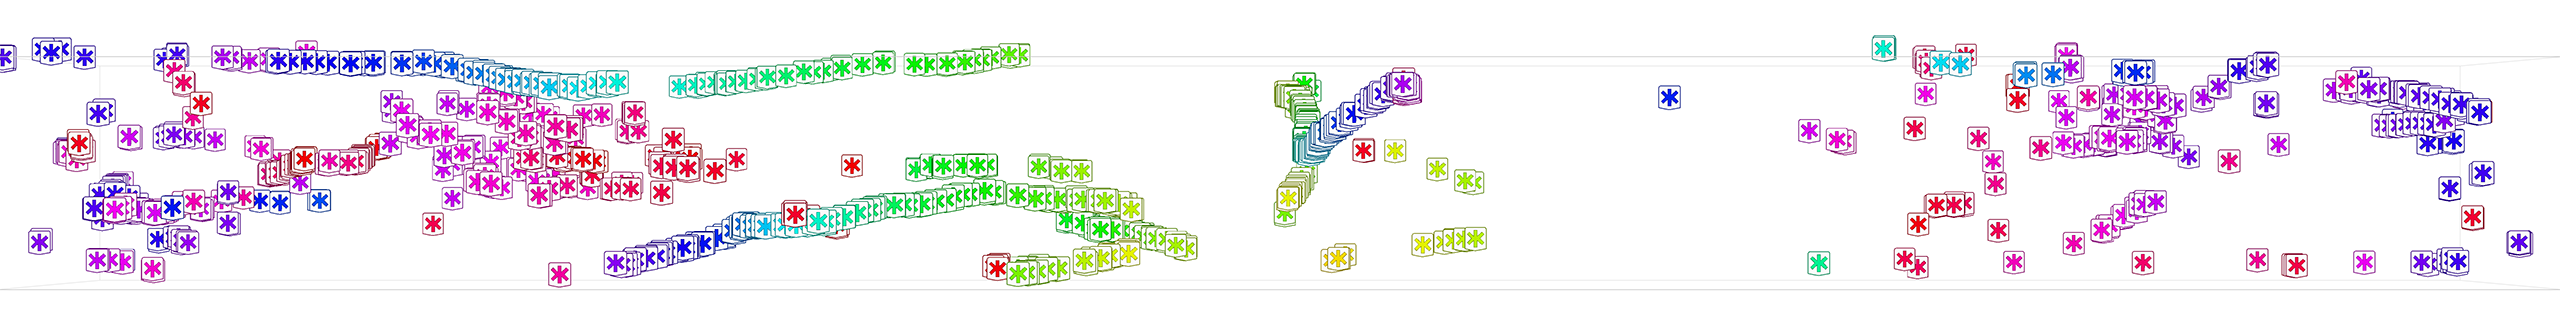
\includegraphics[width=1\textwidth]{eva/EventFlow-Hue-5r-10-ms2-40-bd2-cropped-small-birth}}
				{\caption{Birthereignisse im gesamten Simulationsverlauf. Deutlich sind schnürenartige Verläufe zu erkennen. Die Zeit wird über den Farbwert wiedergegeben und die Glyphgröße beträgt 0,049. Death verhält sich analog.}\label{fig:eva:birth-death-verlauf}}\vss
				\ffigbox[\FBwidth][\FBheight]
				%{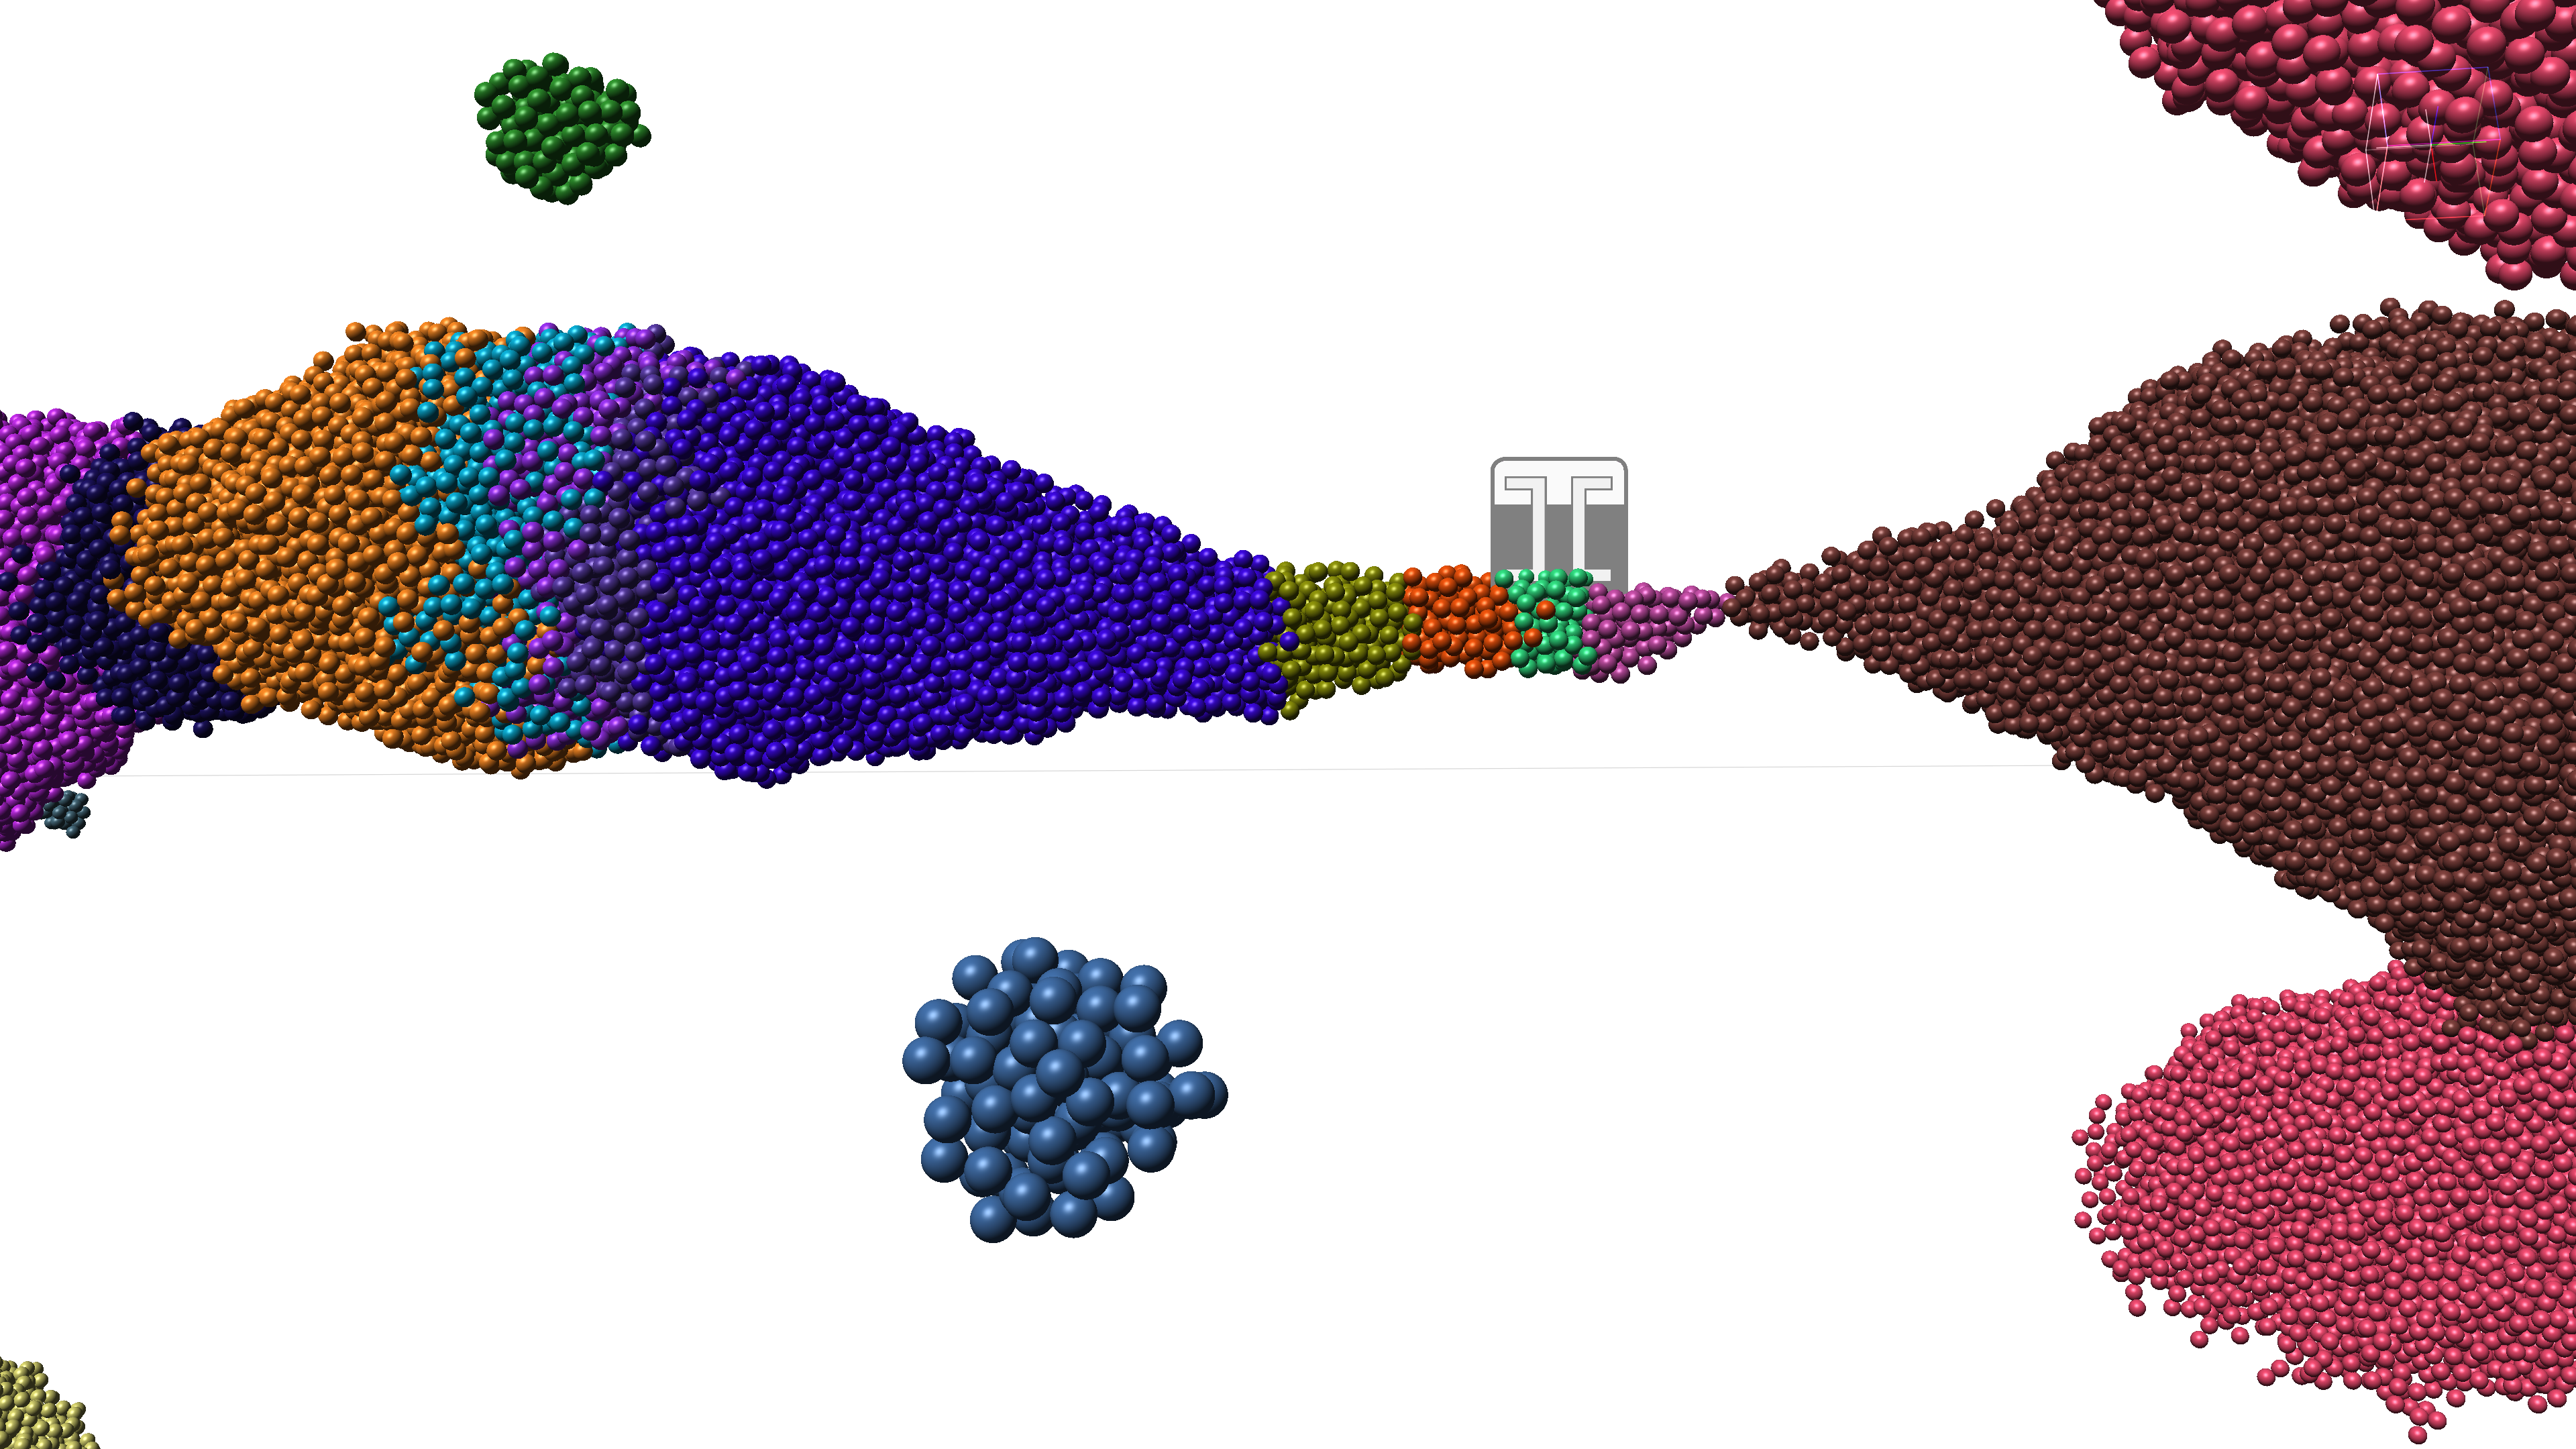
\includegraphics[width=1\textwidth]{eva/spliterkennung-ms2-45-f101}}
				{}
				{\caption{Birth und Death und die zugehörigen \CFDterm{Einpartikelcluster} in der Nahaufnahme mit einer Glyphgröße von TODO.}\label{fig:eva:birth-death}}\vss
			}
		\end{subfloatrow}
	}
	{\caption{Kettenverläufe von Birth- und Deathereignissen bei einem \CFDterm{Partikelradiusmultiplikator} von fünf.}\label{fig:eva:birth-death-flow}}
\end{figure}

%TODO Ketten an Birth/Death Mixen

Diesem Phänomen wird der Name »Nulltiefenwert \CFDterm{Einpartikelcluster}« gegeben, welches in \autoref{sec:nulltiefenwert-einpartikel-cluster} näher beschrieben wird.

\subsection*{Abhängigkeit von den Ereignisparametern}\label{eva:ereignis-quali-param}

\begin{figure}
	\ffigbox[\FBwidth] {
		\begin{subfloatrow}
			\vbox {%
				\ffigbox[\FBwidth][\FBheight]
				{
					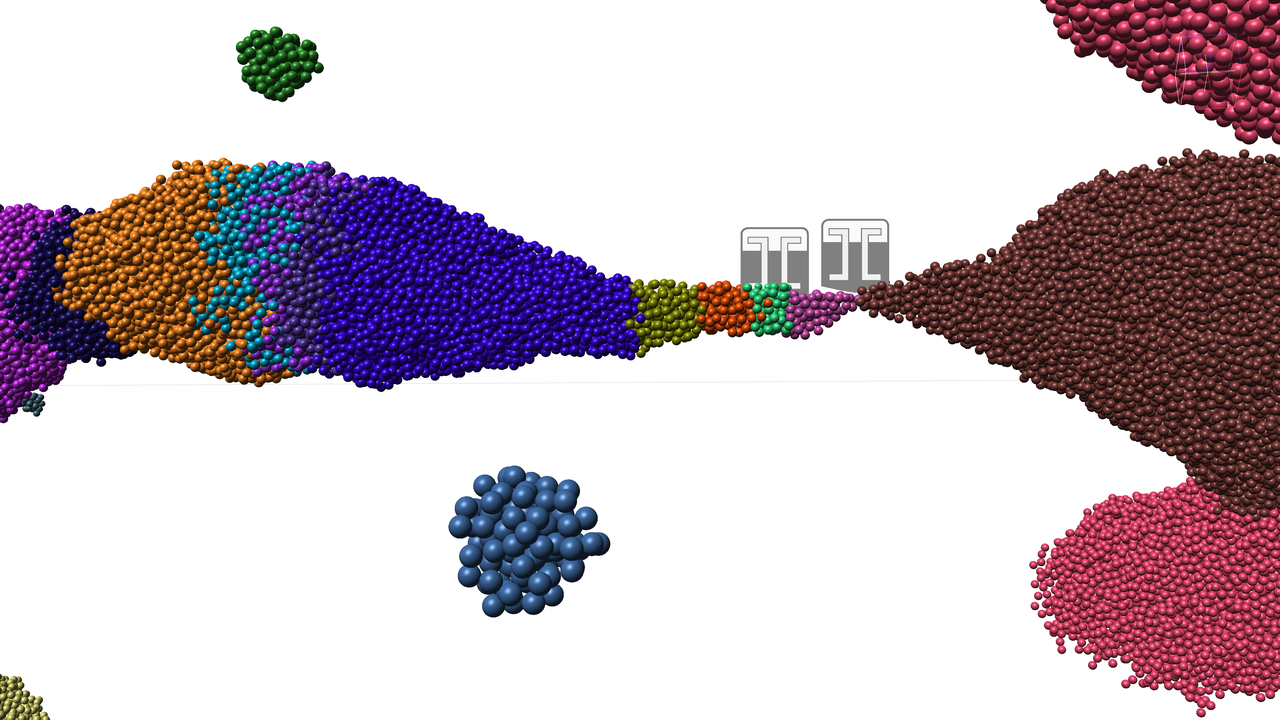
\includegraphics[width=.49\textwidth]{eva/spliterkennung-ms2-40-f101-small}
					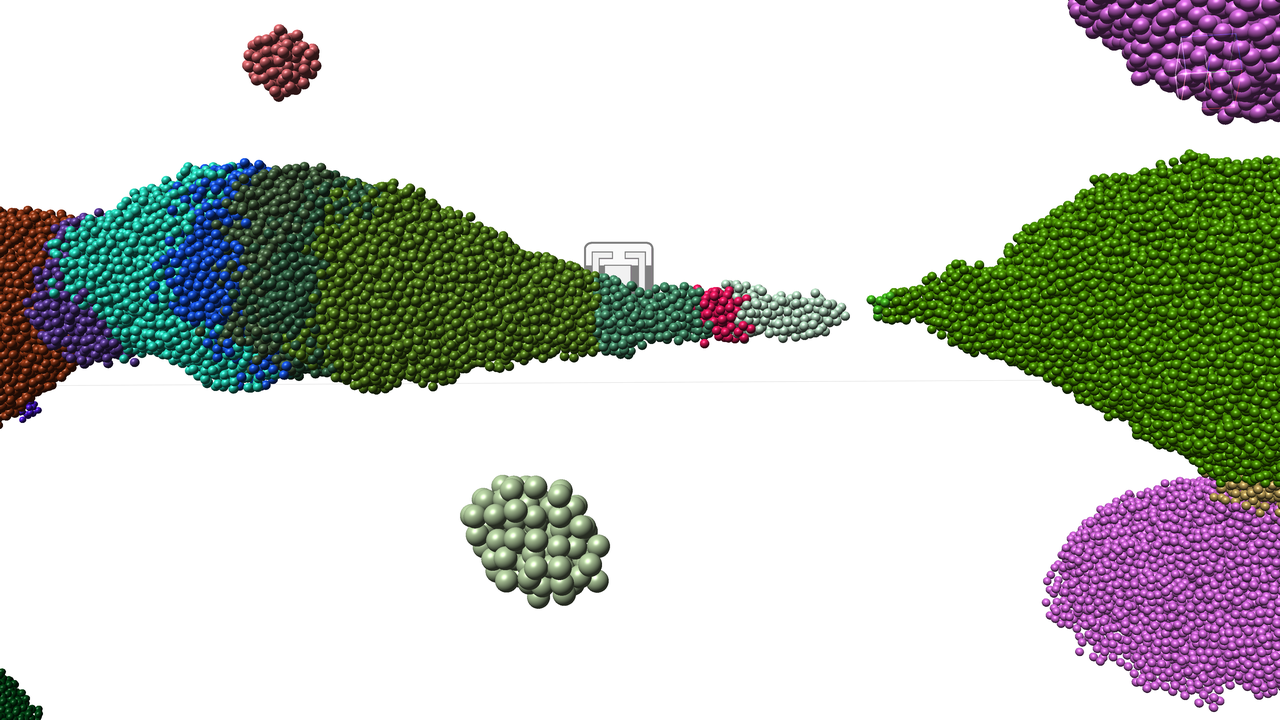
\includegraphics[width=.49\textwidth]{eva/spliterkennung-ms2-40-f102-small}
				}
				{\caption{Das Splitereignis (das Rechte der beiden Splitereignisse) wird erkannt bei einem Anteil von 40\% gemeinsamer Partikel. Das Mergeereignis (rechts) kann als \SECterm{Ereignisrauschen} betrachtet werden.}\label{fig:eva:spliterkennung-ms2-40}}\vss
				\ffigbox[\FBwidth][\FBheight]
				{
					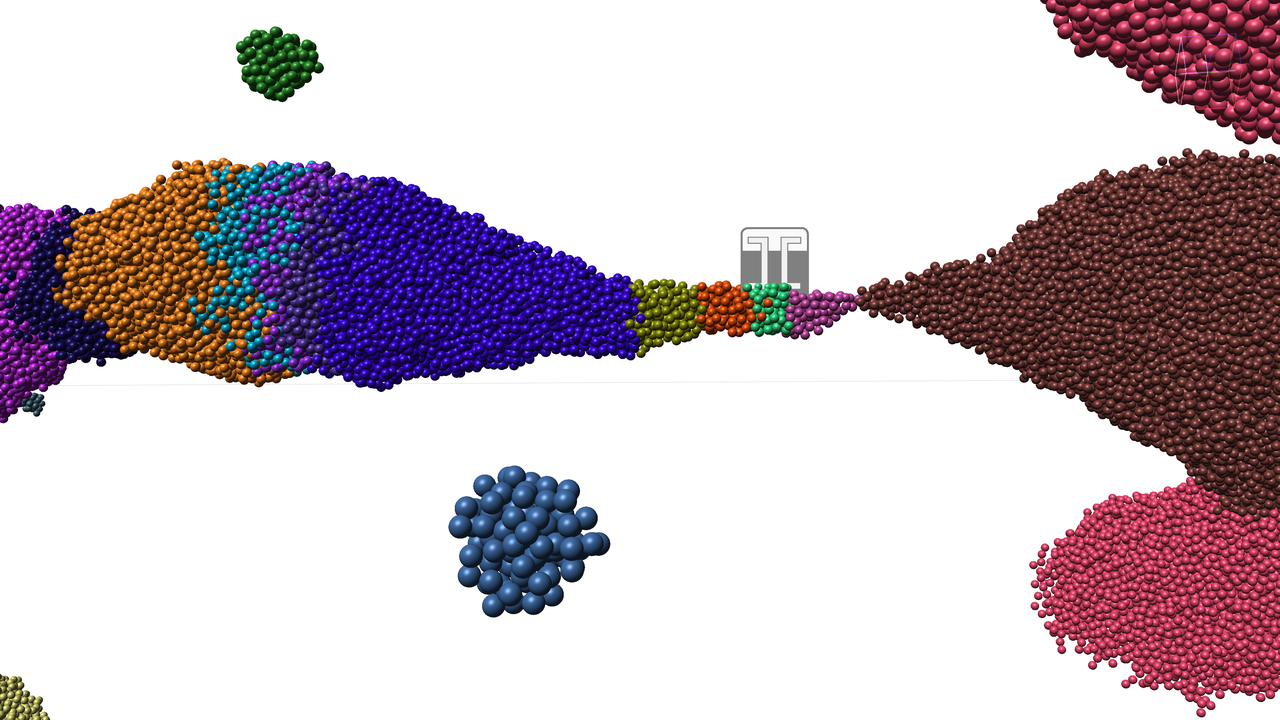
\includegraphics[width=.49\textwidth]{eva/spliterkennung-ms2-45-f101-small}
					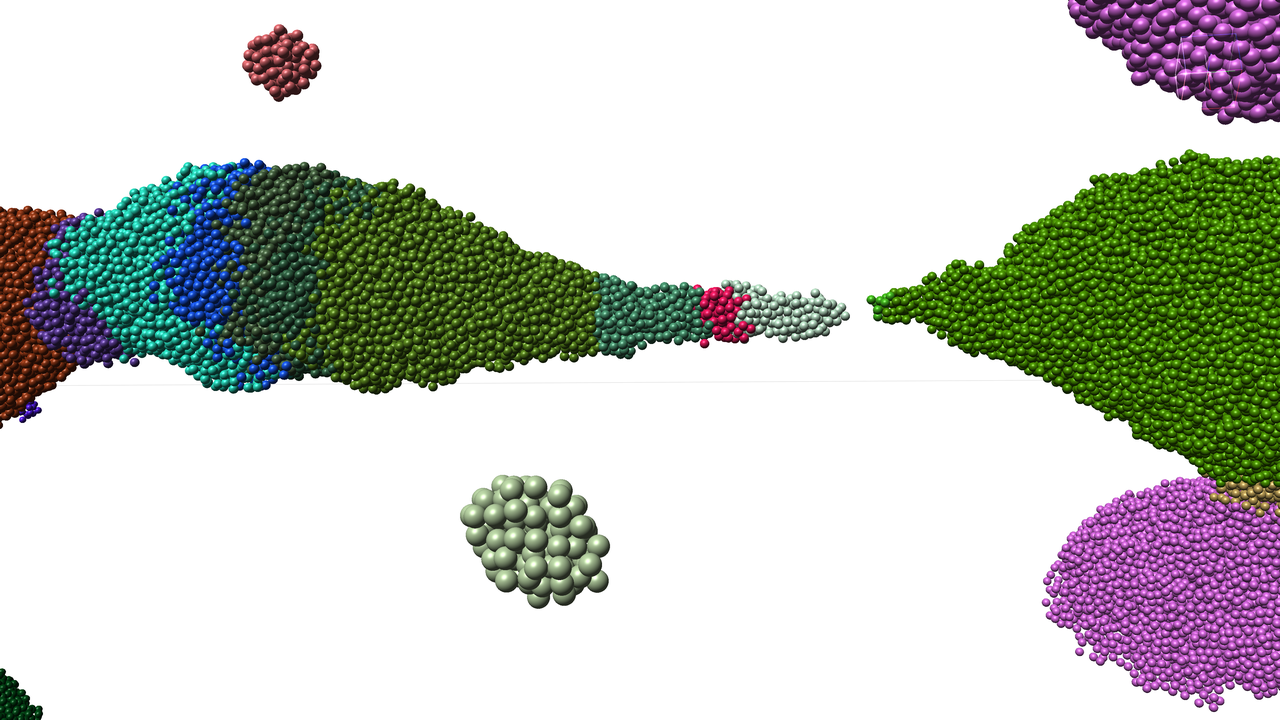
\includegraphics[width=.49\textwidth]{eva/spliterkennung-ms2-45-f102-small}
				}
				{\caption{Das Splitereignis wird bei einem Anteil von 45\% gemeinsamer Partikel nicht erkannt. Gleichzeitig ist jedoch das \SECterm{Ereignisrauschen} geringer, da kein Mergeereignis innerhalb des Filaments auftaucht (rechts).}\label{fig:eva:spliterkennung-ms2-45}}\vss
			}
		\end{subfloatrow}
	}
	{\caption{Abhängigkeit der Erkennung eines Splitereignisses an einem Filament vom Anteil der gemeinsamen Partikel. Der braune Cluster hat sich während des Zeitschritts 101 (links) bereits vom lilafarbenen Cluster gelöst, was im Zeitschritt 102 (rechts) besser zu sehen ist. Durch die zufällige Clusterfärbung verändern sich die Farben zwischen den Zeitschritten. Partikel der Gasphase sind ausgeblendet.}\label{fig:eva:spliterkennung}}
\end{figure}

Der Vergleich in \autoref{fig:eva:spliterkennung} zeigt beispielhaft die erwartete Abnahme der Erkennung der Ereignisse bei restriktiveren Einstellungen der Parameter. So wird die Trennung des Filaments bei einem Anteil gemeinsamer Partikel von 40\% der beiden beteiligten Cluster als Ereignis erkannt, bei einem Anteil von 45\% jedoch nicht mehr, so dass dieser Wert für dieses Filament zu hoch eingestellt ist.
Andererseits ermöglichen restriktivere Werte die Verringerung des \SECterm{Ereignisrauschen}, wie an der Erkennung des Mergeereignisses innerhalb des Filaments zu erkennen ist.

Diese Art der Abhängigkeit der Ereigniserkennung von den gewählten Parametern kann über die gesamte Simulation beobachtet werden.

\section{Visualisierung der Cluster und Ereignisse}

DIESE SEKTION IST NOCH UNFERTIG!

\subsection*{Farbzuweisung der Cluster}
Wenn die Cluster durch die Vererbung der Farben des vorhergehenden Zeitschrittes visualisiert werden, können benachbarte Cluster eine identische Farbe aufweisen, so dass die Clusterunterscheidung erschwert ist. Bei der zufälligen Zuweisung der Farbe geschieht dies nicht. In \autoref{fig:eva:clusterfarbe-rdInteritance} sind deutlich weniger Cluster unterscheidbar als in \autoref{fig:eva:clusterfarbe-allRd}. Aus diesem Grund wurden für die qualitative Analyse nur Datensätze mit zufälligen Clustereinfärbung verwendet.

\begin{figure}
	\ffigbox[\FBwidth] {
		\begin{subfloatrow}
			\vbox {%
				\ffigbox[\FBwidth][\FBheight]
				{\includegraphics[width=1\textwidth]{eva/clusterfarbe-rdInteritance}}
				{\caption{Clusterfärbung mit Vererbung}\label{fig:eva:clusterfarbe-rdInteritance}}\vss
				\ffigbox[\FBwidth][\FBheight]
				{\includegraphics[width=1\textwidth]{eva/clusterfarbe-allRd}}
				{\caption{Zufällig Clusterfärbung ohne Vererbung}\label{fig:eva:clusterfarbe-allRd}}
			}
		\end{subfloatrow}
	}
	{\caption{Clustereinfärbung mit und ohne Vererbung bei Zeitschritt 101. Der \CFDterm{Partikelradiusmultiplikator} beträgt fünf. Partikel der Gasphase sind ausgeblendet.}\label{fig:eva:clusterfarbe}}
\end{figure}

In der Visualisierung als Animation ist der Verlauf der Cluster bei der Farbvererbung jedoch besser zu verfolgen, da bei der zufälligen Zuweisung ein starkes Farbflackern auftritt.

\subsection*{Anordnung}

% Diskussion Vis
\autoref{sec:visualisierung}
Die Komplexität der Ereignisvisualisierung (\vis{Ereignisobjekt}) ist dabei geringer ist als die der Partikel (\vis{Partikelobjekt}). Das hat drei Gründe. Erstens ist die Anzahl der Ereignisse um mehrere Größenordnungen kleiner und zweitens werden im Rahmen dieser Arbeit keine Verbindungen zwischen den Ereignissen analysiert und visualisiert, was die Differenz der Elementanzahl erhält. Schließlich ist drittens, was als Hauptgrund betrachtet werden sollte, die Visualisierung der Ereignisse statisch. Sie behalten im Gegensatz zu den Partikeln dieselbe Position, was sie für den Betrachter während der Animation einfacher erfassbar macht.
Andererseits steigern die in den Glyphen gespeicherten Informationen über den Zeitpunkt und die Ereignisart den Komplexitätsgrad des \viss{Ereignisobjektes}{Ereignisobjekt}, worauf in der Auswertung eingegangen wird.

%Evaluation Vis
In der Übersichtsansicht Komplexitätsgrad Glyphen doof, rangezoom nicht.x




\subsection*{Sichten}
Die Makrosicht dient zur quantitativen Erfassung:
%vorher erklärt, hier bewerten: zum Erkennen von zusammengehörigen und alleinstehenden Elemente, der Struktur im Ganzen. Individuelle Verbindungen sind dabei nicht relevant.

Die Mikrosicht zur qualitativen Erfassung 

(siehe \autoref{sec:related-visFilter})


\subsection*{Glyphdesign}
%TODO Umfrageergebnisse einbinden!

Ein Vorschlag eines Teilnehmers lautete, die ikonische Darstellung des Birthereignisses mit den symbolischen Darstellungen der drei anderen Ereignisse zu kombinieren, da der Teilnehmer »den Kreis nur nach Ausschlussprinzip« zuordnen konnte. Hingegen sagen die Wert, dass der Kreis BLABLA

Erfolg der Glyphgestaltung.



ALT:
- qualitative Umfrage Erkennung der Symbole: Tester (Vorstellung im Bekannten- und Freundeskreis) haben gezeigt, dass sie den Symbolen die korrekte Semantik zuordnen, bei der abstrakten Vorstellung fiel die Zuordnung wesentlich ungenauer aus.


\subsection*{Glyphdarstellung im Partikelraum}\label{sec:eva:glyphdarstellung}

Die in \autoref{sec:vis:glyph-pos} getroffene Annahme, dass die Positionierung des Glyphen oberhalb des Ereignisses intuitiv sei, wurde ebenfalls mit der Umfrage überprüft. Dazu wurde jeweils ein Partikel unter die Spitze, knapp über die Spitze und in die Mitte des Glyphen platziert. Überraschenderweise wurde der Annahme durch eine große Mehrheit widersprochen, denn für die implementierte Variante entschieden sich mit zehn Teilnehmern nur 16\% der Befragten. Eine Platzierung des Partikels knapp oberhalb der Spitze wurde zwar lediglich von zwei Personen favorisiert, dafür entschieden sich 46 der Teilnehmer (75\%) für die Positionierung in der Mitte des Glyphen.

Ein Kommentar bewertet den hohen Komplexitätsgrad des \viss{Ereignisobjektes}{Ereignisobjekt} in der Makrosicht als negativ und spricht von einer »überladenen Glyphdarstellung, die unter Verdeckungen leidet«. Dies ist der Darstellung in der Umfrage geschuldet, da dort die Makrosicht gewählt wurde und aufgrund der statischen Darstellung als Bild mit begrenzter Zoommöglichkeit eine große Glyphgröße gewählt wurde. In der Anwendung können die Glyphen durch den Nutzer skaliert werden, da das \MMStruktur{StaticRenderer Modul} einen entsprechenden Parameter besitzt (siehe \autoref{sec:renderer}).

- schlechte Sichtbarkeit bei gleichzeitiger Ansicht von Partikeln und Events, ClipPlane bei SimpleSphereRenderer hilft etwas %TODO Beispielscreenshot

%TODO Qualitativ



\section{Ressourcenverbrauch}\label{sec:eva:ressourcen}
\begin{figure}
	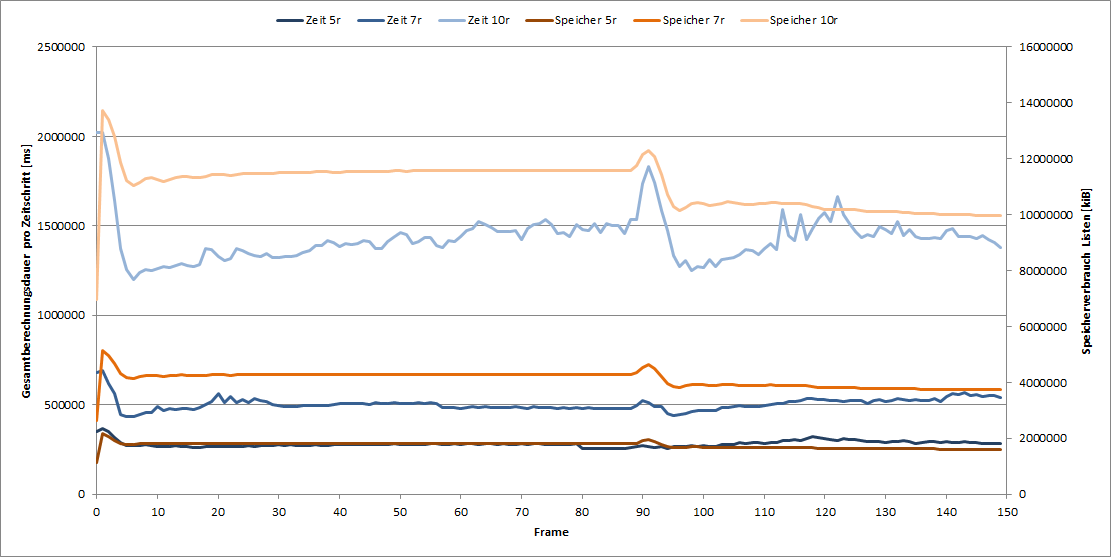
\includegraphics[width=1\textwidth]{eva/ressourcen}
	\caption{Ressourcenverbrauch über alle Zeitschritte in Abhängigkeit des \CFDterms{Partikelradiusmultiplikators}{Partikelradiusmultiplikator}. Der Speicherverbrauch spiegelt nur die Listengröße und nicht den durch die Berechnungen benötigten Speicher wider.}\label{fig:eva:ressourcen}
\end{figure}

In \autoref{fig:eva:ressourcen} ist wiederholt eine starke Abhängigkeit vom \CFDterm{Partikelradiusmultiplikator} bei der Nachbarschaftssuche festzustellen. Mit größerem Suchvolumen nehmen Zeit- und Speicherverbrauch stark zu. Der aufgezeigte Speicherverbrauch spiegelt lediglich die Größe der die Datenstrukturen enthaltenen Listen wider. Bei der Berechnung hat der Prozess mit dem gegeben Datensatz und ohne Visualisierung bis zu 13 \gls{GiB} bei einem Multiplikator von zehn benötigt.

Der Ressourcenverbrauch ist über den Zeitraum annähernd gleichbleibend, bis auf zwei Ausnahmen. Bei der Trennnung und beim Zusammenstoß der Flüssigkeitsfronten ist er stark erhöht, was auf die erhöhte Anzahl an Nachbarschaftsbeziehungen durch die dichte Packung der Partikel in den Fronten sowie die erhöhte Anzahl an Clustern zu diesem Zeitpunkt (siehe \autoref{sec:eva:cluster}) zurückzuführen ist. Dies lässt sich gut in \autoref{fig:eva:ressourcen-berechnungsschritte} erkennen. Vor allem die Nachbarschaftssuche benötigt deutlich länger und der Speicherplatz für die Partikelliste ist größer, da die durchschnittliche Anzahl von Nachbarn pro Partikel aufgrund der dichteren Nähe vieler Partikel zueinander während dieser Zeiten höher ist.

\begin{figure}
	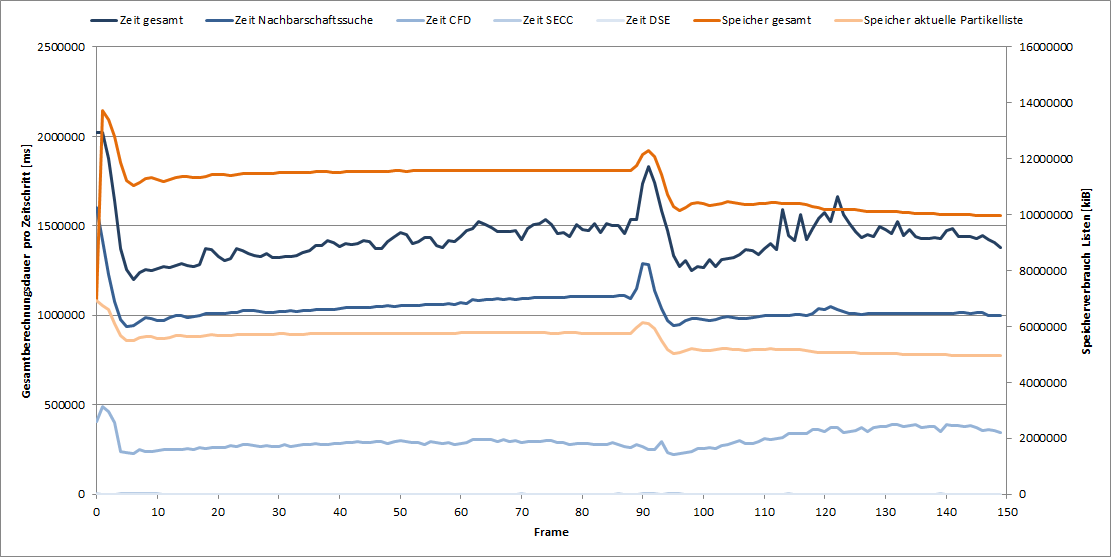
\includegraphics[width=1\textwidth]{eva/ressourcen-berechnungsschritte}
	\caption{Ressourcenverbrauchsverteilung der Berechungsschritte über den gesamten Zeitraum bei einem \CFDterm{Partikelradiusmultiplikator} von zehn. Die Speicherdaten für \SECC sowie für \gls{dse} wurden ausgeblendet, da ihre geringen Werte wie auch ihre Zeitdaten unerheblich sind.}\label{fig:eva:ressourcen-berechnungsschritte}
\end{figure}

Nach dem Zusammenstoß beider Fronten kann eine leichte Abnahme der durchschnittlichen Nachbarn pro Partikel im Vergleich zur Zeit vor dem Zusammenstoß beobachtet werden. Das ist ein Indiz auf mehr Randpartikel mit weniger Nachbarn und damit ein erhöhtes Tröpfchenaufkommen. Diese Vermutung wird durch ein stark erhöhtes Aufkommen von \CFDterm{Mindestgrößencluster} nach dem Zusammenstoß in \autoref{fig:disk:merge-min-one-size} gestützt. Weiterhin könnten auch mehr Partikel in die Gasphase übergegangen sein als zuvor, was durch die Messungen in \autoref{fig:eva:gasparticles} bestätigt wird.

\begin{figure}
	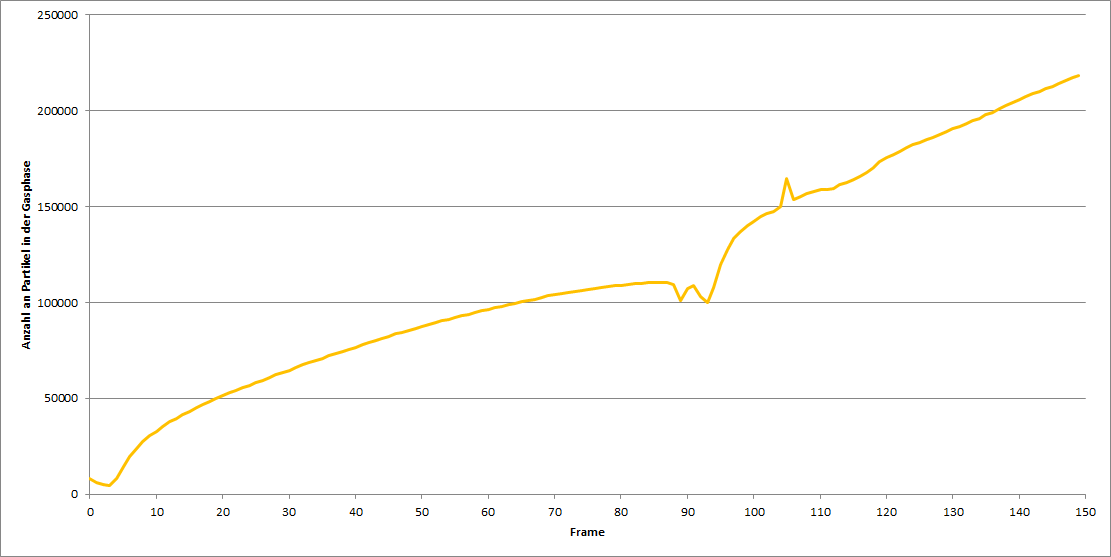
\includegraphics[width=1\textwidth]{eva/gasparticles}
	\caption{Anzahl der Partikel in der Gasphase über den Zeitraum der Simulation verteilt.}\label{fig:eva:gasparticles}
\end{figure}

Der nahezu halbierte Speicherverbrauch der Partikelliste des aktuellen Zeitschrittes und dem Gesamtspeicherverbrauch liegt daran, dass die Partikelliste des vorhergehenden Zeitschrittes in den Gesamtverbrauch einfließt. Hingegen sind die anderen Listen für die Cluster, \SECterm{Partnercluster} sowie Ereignisse mit einer Größe von wenigen \gls{kiB} vernachlässigbar klein und wurden daher ausgeblendet.

Diese Daten liefern eine wichtige Erkenntnis. Die Nachbarschaftssuche benötigt mit großem Abstand die meiste Zeit, danach folgt der \CFD mit etwa ein Viertel des Zeitverbrauchs. Die anderen Schritte liegen mit einer Dauer von maximale zwei Sekunden für den \SECC und wenigen Millisekunden für die Ereignisheuristik um zwei und mehr Größenordnungen darunter.

Der Speicherverbrauch der Listen ist mit maximal 1,4 \gls{GiB} bei einem \CFDterm{Partikelradiusmultiplikator} von zehn überschaubar. Der in Stichproben registrierte wesentlich höhere Gesamtspeicherverbrauch des Berechnungsprozesses zwischen elf und 13 \gls{GiB} ist vor allem auf das Vorhalten des gesamten Datensatzes der Simulation in Form des \gls{mmpld} im Speicher zurückzuführen (über fünf \gls{GiB}) sowie auf den hohen Verbrauch bei der Durchsuchung des kD-Baums.


\chapter{Diskussion der Ergebnisse}\label{sec:diskussion}

\section{Einfluss der Nachbarschaftssuche}\label{sec:eva:nachbarschaftssuche}

Wie die Evaluation zeigt, hat die bei der Nachbarschaftssuche gewählte, maximale Reichweite einen maßgeblichen Einfluss auf alle Berechnungsschritte. Deswegen ist die Diskussion des \CFDterms{Partikelradiusmultiplikators}{Partikelradiusmultiplikator} und die damit verbundenen Phänomene bedeutend für diese Arbeit.

\subsection*{Flüssigkeitspartikel ohne Cluster und erhöhtes Ereignisrauschen bei zu kleiner Nachbarschaftssuche}
In \autoref{sec:eva:cluster} ist zu sehen, dass bei kleinem \CFDterm{Partikelradiusmultiplikator} nur sehr kleine Cluster erkannt werden, denn das Volumen für die Nachbarschaftssuche ist so klein, dass viele Partikel der Flüssigkeitsphase keine Nachbarn besitzen. Weiterhin ist die Berechnungsgeschwindigkeit bei einem vierfachen Modifikator 20\% geringer als mit einem dreifachen, so dass der in der Benutzeroberfläche zugelassene Minimalwert für den Radiusmultiplikator vier beträgt. Ein weiterer Grund ist, dass ein sehr kleines Suchvolumen das Aufkommen winziger Cluster stark erhöht, da die Partikel der flüssigen Phase nicht dicht gepackt sein müssen und so nebeneinanderliegende Partikel nicht als solche erkannt werden. 
Damit ist es wahrscheinlicher, dass der \CFD \autoref{sec:fast-depth} sie unterschiedlichen Clustern zuordnet, weil räumlich benachbarte, aber bei der Nachbarschaftssuche nicht als Nachbarn erkannte Partikel bei der Suche nach dem nächsten, tiefer liegenden Partikel nicht beachtet werden (siehe \autoref{fig:eva:cluster}). Eine erhöhte Clusteranzahl innerhalb von Zusammenhangskomponenten führt zu einer erhöhten Anzahl von detektierten Ereignissen. Wenn der Nutzer den Einfluss kleiner Cluster ignorieren möchte und sie als \SECterm{Ereignisrauschen} statt als gewinnbringende Information betrachtet, so ist ein kleines Suchvolumen bei der Nachbarschaftssuche von Nachteil.

\subsection*{Gaspartikelcluster bei der Clusterreduktion}  %MergeClusters produces adjacent gas particle clusters theory

Wenn andererseits der \CFDterm{Partikelradiusmultiplikator} zu groß gewählt wird (fünffacher Radius oder höher), können auch Partikel der Gasphase Nachbarn erhalten und werden im \CFD Clustern zugeordnet. Dies wiederum kann dazu führen, dass beim Reduzieren der kleinen Cluster \autoref{sec:clusterreduktion} die Partikel in Clustern mit nur diesem einen Partikel zurückbleiben. Das liegt darin begründet, dass die Clusterreduktion begrenzte Iterationsschritte aufweist. Falls der von den umliegenden Cluster am Weitesten entfernte Partikel als erstes ausgewählt wird, weisen die umliegenden Partikel noch denselben Cluster auf. Wenn die Suche nach drei Nachbarschaftsebenen abbricht und die durchsuchten Partikel alle denselben Cluster aufweisen, verbleibt der Partikel im aktuellen Cluster. Hingegen werden die umliegenden Partikel aufgrund der geringeren Entfernung zu den benachbarten, größeren Clustern in diese aufgenommen. So verbleibt der zuerst ausgewählte Partikel als einziger im Cluster. Das führt in der Ereigniserkennung \autoref{sec:ereigniserkennung} zu falschen Birth und Death Erkennungen.
Allerdings ist dieser Fehler nicht aufgetreten, es werden keine einzelnen Partikel oder kleine Partikelgruppen durch die Clusterreduktion erzeugt. Das kann durch den Vergleich der Einpartikel- sowie der minimalen Cluster direkt nach der Clusterbildung mit deren Anzahl nach der Clusterreduktion überprüft werden. In \autoref{fig:disk:merge-min-one-size} bleibt in allen Zeitschritten die Anzahl nach der Clusterreduktion gleich oder ist geringer als vorher. Damit ist gezeigt, dass durch die Reduktion keine Gaspartikelcluster erzeugt werden.

\begin{figure}
	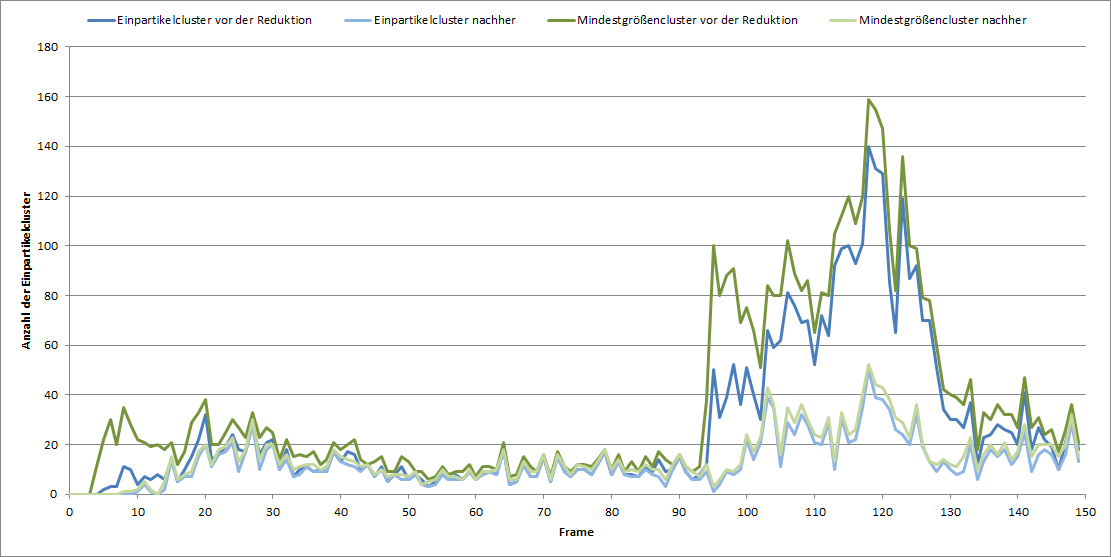
\includegraphics[width=1\textwidth]{eva/merge-min-one-size}
	\caption{Anzahl der Mindestgrößencluster (grün) sowie der \CFDterm{Einpartikelcluster} (blau) vor und nach der Clusterreduktion bei einem \CFDterm{Partikelradiusmultiplikator} von fünf.}\label{fig:disk:merge-min-one-size}
\end{figure}

%Umgangen wird dieser mögliche Fehler bei der Bestimmung der Clusterzusammenhänge \autoref{sec:clusterzusammenhaenge} durch das Herausfiltern von Clustern mit einer Partikelanzahl von eins.
Das Ausbleiben dieses Fehlers lässt sich auf die verwendete minimale Clustergröße von maximal zehn Partikeln zurückführen. Somit ist die dreifache Iteration der Clusterreduktion ausreichend. Hingegen wird mit höheren Mindestclustergrößen der Fehler verstärkt auftreten. Das kann leicht vermieden werden, indem die Anzahl der durchsuchten Nachbarschaftsebenen erhöht wird, etwa durch die Umstellung der Clusterreduktion in einen iterativen oder rekursiven Prozess, dessen Durchgänge abhängig der gewählten Mindestclustergröße abhängig sein können.

\subsection*{Gaspartikel in Clustern bei großen Radien}

Zur Beschleunigung des \CFD werden alle Partikel, die beim Suchen entlang des Pfades getroffen wurden, ebenfalls zum Cluster hinzugefügt. Diese Beschleunigung kann Fehler verursachen, wenn der \CFDterm{Partikelradiusmultiplikator} bei der Nachbarschaftssuche (siehe \autoref{sec:nachbarschaftssuche}) groß gewählt wurde, da so auch Gaspartikel am Rand von Clustern mit hinzugefügt werden. Diese Fehler sind jedoch vernachlässigbar, da die Heuristik der Ereigniserkennung \autoref{sec:ereigniserkennung} Mengen betrachtet und somit einzelne Gaspartikel in der Clustergruppe einen geringen Einfluss auf das Ergebnis haben.

\subsection*{Nulltiefenwert Einpartikelcluster Phänomen}\label{sec:nulltiefenwert-einpartikel-cluster} %zero signed distance one size clusters phenomenon 

Aufgrund der Abbruchbedingung der Traversierung über die \contours{Tiefenwerte}{Tiefenwert} kann es passieren, dass Partikel mit denselben \contours{Tiefenwerten}{Tiefenwert} in einzelne, separate Cluster eingeteilt werden, die alle nur diesen einen Partikel enthalten. Da Gaspartikel vom \CFD aussortiert werden und der Algorithmus für das Eintreten dieses Falls keine tieferen Nachbarn finden darf, müssen die Partikel einen Tiefenwert von null aufweisen. Damit nebeneinander angeordnete Partikel diesen Tiefenwert aufweisen können, muss der Cluster sehr klein sein.
Die Überprüfung der Positionen der betroffenen \CFDterm{Einpartikelcluster} bestätigt diese Annahme. Da diese Daten sehr umfangreich sind und sich schwer statisch visualisieren lassen, wird hierbei auf die digitalen Protokolle des \CFD in den einzelnen Messungen verwiesen. %siehe CFD.csv bei den Messungen
Dieses Phänomen tritt ab dreifachem Partikelradius in der Nachbarschaftssuche auf, Bei kleineren Radien werden die nebeneinanderliegenden Partikel mit einem \contour{Tiefenwert} von null nicht als Nachbarn erkannt. Da diese Partikel somit nachbarlos sind, werden sie vom \CFD ignoriert und nicht in Cluster eingeteilt.

Diese Phänomen bewirkt die Bildung zahlreicher Birth- und Deathereignisse (siehe \autoref{sec:eva:ereignisse-quali-verlauf}). Da diese Cluster jedoch korrekt erkannt werden, wird dies nicht als Fehler betrachtet. Eine Einordnung als \SECterm{Ereignisrauschen} kann hingegen vorgenommen werden.

\section{Farbgebung der Glyphen}
DIESE SEKTION IST NOCH UNFERTIG!

Die Umfrage über die Positionierung des Glyphen relativ zum Ereignis widerspricht der Implementation und scheint damit dem in \autoref{sec:related-praattentiveWirkung} formulierten Ziel zur Förderung der präattentiven Wahrnehmung entgegen zu wirken. Dem kann begegnet werden, indem entweder die Glyphdarstellung durch einen deutlich spitzer zulaufender Pfeil am unteren Rand eindeutiger gestaltet wird oder die Positionierung des Glyphs mittig über dem Ereignis erfolgt.

%TODO
Farbverläufe: Feedback Umfrage
Erfahrungswerte mit Farbe gekoppelt, so dass eine Farbgebung nach bekanntem Muster (z.B. Verkehrsampel) sinnvoller ist.


\section{Verdeckung der Glyphen}
Wie in der Evaluation in \autoref{sec:eva:glyphdarstellung} gezeigt, wurde in der Umfrage die Verdeckung der Glyphen untereinander bei starken Zoomfaktoren bemängelt. Dies ist der Darstellung in der Umfrage geschuldet, da in der Anwendung die Glyphen skaliert werden können. Falls auch das nicht ausreicht, kann die Einführung einer Beziehungssicht nach Lima helfen (siehe \autoref{sec:related-visFilter}). Um diese Sicht herstellen zu können, kann nach Gleicher et al (siehe \autoref{sec:related-visAnordnung}) eine Kombination von Gegenüberstellung und expliziter Verschlüsselung genutzt werden und so durch die Trennung des Ereignisraums vom Raum der Partikel die Bindung der \viss{Ereignisglyphen}{Ereignisglyph} an die Position aufgehoben werden, wie es die in dieser Arbeit vorgeschlagene \vis{Strukturereignistaxonomie} ermöglicht (siehe \autoref{sec:strukturereignistaxonomie})
Weiterhin zeigte sich bei der Nutzung des Programms das Problem, dass die Glyphen durch die Partikel verdeckt werden, was dadurch ebenfalls beseitigt werden kann. %siehe auch Ausblick.


\section{Optimierung des Ressourcenverbrauchs durch Parallelisierung}
Die Nachbarschaftssuche ist der zeit- und speicherintensivste Schritt. Eine Parallelisierung der Schleifen für die Partikel wäre wünschenswert, da die Partikel voneinander unabhängig behandelt werden und jeder einzelne Schleifendurchgang rechenaufwändig ist. Dies tritt bei der Beachtung der periodischen Randbedingungen und dem damit verbundenen, achtfachen Aufruf des Suchalgorithmus des kD-Baums umso hervor. Allerdings haben Versuche mit \tool{OpenMP} als auch mit der \PPL gezeigt, dass die \ANN bei der Parallelisierung durch eines der beiden Verfahren trotz rein lesenden Zugriffs Zugriffsfehler aufweist, da jeder Thread auf denselben Baum und dessen Zeiger zugreift. Das Kopieren des Suchbaums für jeden Thread könnte eine mögliche Lösung sein, die unabhängigen Suchen würden mit steigender Partikel- und Threadanzahl jedoch sehr viel Speicher verbrauchen (siehe \autoref{sec:eva:ressourcen}).
Der Blocker für die Parallelisierung mit der \ANN ist allerdings, dass sie während der Programmlaufzeit für alle Suchstrukturen denselben Speicherbereich nutzt und ihn dadurch auch beim Löschen einzelner Suchstrukturen nicht deallokiert \cite[S.~8]{mount2010ann}. Somit ist \ANN für eine parallele Nutzung nicht geeignet und ein Wechsel zu einer anderen Bibliothek ist empfehlenswert, wie beispielsweise zu \FLANN \cite{ohara2013annAlgo} \cite{wijewardena2014annPerformance}.

Bei der Clusterbildung als zweitlängster Schritt kann die Verarbeitung für jeden Partikel parallelisiert werden. Allerdings wird die Beschleunigung nur gering oder sogar negativ ausfallen. Zum Einen müssen die Clustererstellung sowie die Clusterzuordnung des \CFDterms{Wurzelpartikels}{Wurzelpartikel} threadsicher umgestaltet werden, zum Beispiel mittels Mutex-Verfahren, um eine mehrfache Clusterzuweisung auf denselben Partikel zu vermeiden. Das führt zu einer Verringerung der Parallelisierungseffizienz, da die Prozesse gegenseitig aufeinander warten müssen, bis die Erstellung und Zuordnung abgeschlossen ist. Zum Anderen müsste das Hinzufügen der traversierten Partikel zum Cluster entfernt werden, wodurch die auch in vorhergehenden Schritten getroffenen Partikel untersucht werden müssen, was vor allem bei langen Traversierungspfaden aufgrund der sequentiell ablaufenden Traversierung die Effizienz stärker senken kann, als die durch die Parallelisierung hinzugewonnene.

Die Clusterreduktion ist beim Durchlaufen der Partikel parallelisiert und dadurch kann auf dem Zweikernprozessor mit vier Threads des Testsystems in Stichproben eine Geschwindigkeitsverbesserung von über 15\% festgestellt werden (Frame 75 5622 \gls{ms} zu 6733 \gls{ms}, Frame 76 5631 \gls{ms} zu 6802 \gls{ms}). Die geringe Skalierung ist damit zu erklären, dass nur ein Bruchteil der Partikel reduziert wird (in den Stichprobe der Frames 75 und 76 sind es 66 bzw. 55 Partikel, damit 0,03\% aller Partikel). Die Berechnung der Winkel zu den benachbarten Clustern geschieht in einer Schleife innerhalb des Durchlaufes eines Partikels und ist noch einmal parallelisiert, was aufgrund der geringen Clusteranzahl nur in einem minimalen Geschwindigkeitsgewinn von unter 4\% resultiert. Die Mutex in beiden Schleifen (Zählvariable und minimaler Winkel) haben keinen messbaren Einfluss auf die Geschwindigkeit.
Die Parallelisierung der drei einzelnen Suchschritte nach den benachbarten Clustern ist nicht sinnvoll, da dort zum Ersten lediglich Vergleiche und Inkrementationen durchgeführt werden und zum Zweiten das Hinzufügen des ermittelten Wertes zum der die benachbarten Cluster enthaltenen Container nicht Threadsicher ist und durch einen Mutex geschützt sein muss. Versuche haben gezeigt, dass der bei der Parallelisierung erzeugte Verwaltungsaufwand den Vorgang sogar verlangsamt. Bei Frame 75 wird ohne Parallelisierung der Clustersuche eine Dauer von 6791 \gls{ms} und mit Parallelisierung eine Dauer von 8711 \gls{ms} ermittelt, respektive bei Frame 76 6688 \gls{ms} zu 8394 \gls{ms}.
%TODO-- Verlinkung SECalc Parallelisierungseinfluss von mergeClusters.csv, nicht notwendig!

Beim Clustervergleich sowie der Ereigniserkennung wäre aufgrund des geringen Berechnungsaufwandes, des nötigen Mutex-Verfahren der Listen sowie der sequentiell zu erfolgenden Ausgabe eine Parallelisierung in der Geschwindigkeit kaum spürbar bzw. sogar nachteilig.

%Falsch: In der Implementation wird so oft wie möglich der Parallelmodus von libstdc++ genutzt, um den Zugriff auf die Listen zu beschleunigen. %TODO nicht standardmäßig durch vc++ unterstützt? url https://gcc.gnu.org/onlinedocs/libstdc++/manual/parallel\_mode.html
%Gelegentlich werden OpenMP Direktiven unmittelbar an den Schleifen verwendet.


\section{Optimierung der Algorithmen}\label{sec:disc:optimierungAlg}
Der \CFD kann optimiert werden, indem beim Treffen auf den ersten Partikel, der einem Cluster angehört, die Suche beendet ist und die Clusterzuweisung erfolgt. Dies kann enorme Geschwindigkeitszuwächse des Algorithmus bewirken, ohne dass dessen Qualität beeinflusst wird.

Die \SECC kann um einen Clusternachbarschaftsgraphen erweitert werden. Dieser speichert wie in \autoref{sec:clusterzusammenhaenge} vorgeschlagen für jeden Zeitschritt die Nachbarschaften der Cluster. In Kombination mit dem Mengenvergleich können so mit einer messbaren Wahrscheinlichkeit die Cluster zugeordnet werden (siehe \autoref{sec:visualisierung:cluster}). %Redundant: Die Zuordnung könnte verbessert werden durch Berücksichtigung eines Durchschnittswert der enthaltenen Partikel IDs mit einer Toleranzgrenze, die experimentell bestimmt werden müsste.
Dies stellt eine weitere Option bereit, um die Strukturereignisse daraus abzuleiten.



\chapter{Zusammenfassung}
%Kurzzusammenfassung/Abstract ausführlicher, auf Details eingehen

Diese Arbeit stellt eine auf den Ideen der Skelettextraktion und \contours{Konturbäumen}{Konturbaum} aufbauende Möglichkeit vor, um aus Punktdaten Strukturen zu erkennen. Diese Strukturen werden genutzt, um daraus Strukturereignisse abzuleiten.

Die Berechnungen lassen mit Hilfe ihrer sowohl quantitativen als auch qualitativen Ausgabe Erkenntnisse über die Veränderung der Strukturen während der Simulation zu, da die Anzahl der Cluster und die Verteilung der Partikel stark auf Topologieänderungen reagiert. Der Nutzer kann Parameter ändern, um etwa \SECterm{Ereignisrauschen} zu verringern und durch die Möglichkeit, die Berechnungen permanent zu speichern, auch schnell zwischen den Parametern für die einzelnen Berechnungsschritte wechseln und so die Nachteile der individuellen Einstellungen auszugleichen. Beispielsweise die Erfassung aller wesentlichen Ereignisse durch einen kleinen \CFDterm{Partikelradiusmultiplikator} und einen niedrigen Schwellwert für die Anteile gemeinsamer Partikel mit dem Nachteil von starkem \SECterm{Ereignisrauschen}. Dagegen können restriktivere Einstellung mit höheren Schwellwerten geringes \SECterm{Ereignisrauschen} verursachen mit dem Nachteil, einige wesentliche Ereignisse nicht zu erfassen (siehe \autoref{sec:eva:ereignis-param}, \autoref{eva:ereignis-quali-param}).

Trotz dessen, dass die erhoffte Umsetzung der Berechnungen mit \contours{Konturbäumen}{Konturbaum} und ihren bereitgestellten Schwellwerten nicht erfolgen konnte, wurde die Zielstellung, Strukturveränderung mittels \viss{Ereignisglyphen}{Ereignisglyph} abzubilden, durch die Entwicklung eigener Algorithmen in Form des \CFD und der \SECC sowie der darauf aufbauenden \SECterm{Ereignisheuristik} erreicht. Diese geben dem Nutzer Mittel in die Hand, Schwellwerte zu setzen, die die Qualität und Anzahl der erkannten Ereignisse stark beeinflussen. Weiterhin ergab eine Umfrage unter Experten und Laien, dass die Bedeutung der Glyphen intuitiv eingeschätzt werden kann und die Prozesse, die zu den visualisierten Ereignissen führten, seitens der Experten größtenteils korrekt eingeschätzt werden. Hingegen fällt es schwer, ohne Hintergrundwissen allein durch die Visualisierung Prozesse richtig zu beurteilen (siehe \autoref{sec:eva:ereignisse-quali-verlauf}).

Durch die Clustervisualisierung, die umfangreiche Bereitstellung quantitativer Ergebnisse, die vorgeschlagene \vis{Strukturereignistaxonomie}, mehrere Möglichkeiten zur Glyphdarstellung sowie durch die Auswertung unter Einbeziehung von Laien konnten die geplanten Ziele der Arbeit übertroffen werden. Auch ist das entstandene Plugin in der Lage, Strukturanalysen von Partikeldatensätzen mit einem Skalarfeld für den \contour{Tiefenwert} durchzuführen und mit Hilfe des \viss{Glyphprototypen}{Glyphprototyp} können weitere Überprüfungen zur Verknüpfung von \viss{visuellen Variablen}{visuelle Variable} mit Parametern einer Struktur durchgeführt werden. Verweise und Kurzbeschreibungen befinden sich in \autoref{sec:pluginaufbau} und \autoref{sec:glyphprototyp}.

Ein Problem der entwickelten Algorithmen stellt das \SECterm{Ereignisrauschen} dar, dass bei allen vier Arten der Strukturereignisse auftritt. Weiterhin dauern die Berechnungen zu lang, um in direkt angezeigt zu werden. Auch gibt es Verdeckungen der Glyphen untereinander sowie durch die Partikel, was die Erfassung der Ereignisinformationen erschwert. Im folgenden Kapitel werden diesbezügliche Verbesserungsmöglichkeiten beschrieben.


\chapter{Ausblick}
LISTEN WERDEN NOCH IN FLIESSTEXT UMGEWANDELT!

Zur Verringerung des starken \SECterms{Ereignisrauschens}{Ereignisrauschen} werden vier Modifikationen für die Algorithmen vorgeschlagen.
\begin{itemize}
	\item Clustergröße, die zur Bildung des Ereignisses geführt hat, im Ereignis abspeichern. So kann der Benutzer eine Gewichtung der Ereignisse abhängig von der Clustergröße vornehmen bzw. die Auswirkungen kleiner Cluster dynamisch ausblenden.
	
	\item Die Mindestclustergröße auf wesentlich höhere Werte, zum Beispiel größer 100 einstellen, um das \SECterm{Ereignisrauschen} in Zusammenhangskomponenten zu senken. Voraussetzung dafür ist die Erhöhung der durchsuchten Nachbarschaftsebenen. Dies kann zum Beispiel durch Umwandlung des iterativen Vorgehens in ein Rekursives erreicht werden. Empfehlenswert ist die Skalierung der Rekursionschritte mit der Mindestclustergröße, um die Berechnungsdauer der Reduktion nicht unnötig zu erhöhen. Da kleinere Cluster, die nur eine Zusammenhangskomponente bilden, bei der Reduktion erhalten bleiben, gibt es keinen Verlust dieser Ereignisinformationen.
	Die im Berechnungsmodul vorhandenen Ausgaben der berechneten, quantitativen Daten ermöglichen leicht eine vorangehende statistische Analyse für eine zielgerichtete Einstellung der Mindestclustergröße, etwa durch die Ausgabe der Anzahl von Clustern bestimmter Größen.
	
	\item Einbeziehung von sowohl der Forward- als auch der Backwardsliste bei der Ermittlung von Merge und Split, Vergleich der Durchschnittswerte der Verhältnisse der gemeinsamen Partikel der Elternpartner in der jeweiligen anderen Liste und eine daraus abgeleitete Gewichtung.
	
	\item Nutzung der Nachbarschaften von Clustern, wie mit dem Nachbarschaftsgraphen vorgeschlagen
\end{itemize}

Zusätzliche Erkenntnisse für die Strukturveränderungen können durch, in dieser Arbeit nicht betrachteten, Zusammenhängen zwischen Clustern gebildet werden. Mit den vorhandenen Algorithmen kann das geschehen, indem Cluster über mehrere oder alle Zeitschritte verglichen werden. Dazu kann eine Signatur für jeden Cluster genutzt werden, die beispielsweise aus der Summe der Partikelidentifikatoren gebildet werden kann. Dadurch können Ereignisse zueinander in Beziehung gestellt werden.
	
Weiter ist eine Geschwindigkeitserhöhung der Berechnungen mit den vorhanden Algorithmen umsetzbar. So
	\begin{itemize}
		\item Nachbarschaftssuche: Nutzung von \FLANN o.ä., die Parallelisierung nutzen. \cite{ohara2013annAlgo}
		
		\item Parallelisierung bei Clusterbildung: Mehrere Partikel parallel verarbeiten. Dazu muss die Clusterliste eine vordefinierte Größe aufweisen, was bereits durch die Speicherplatzreservierung implementiert ist. Des Weiteren müssen die Sprünge in der Schleife durch Abfragen ersetzt werden, was einen geringen Einfluss auf die Geschwindigkeit hat. Jedoch muss die Clustererstellung sequentiell erfolgen, um eine mehrfache Clusterzuweisung auf denselben Partikel zu vermeiden, was zu einer Verringerung der Parallelisierungseffizienz führt, da die Prozesse gegenseitig aufeinander warten müssen, bis die Clusterzuordnung des \CFDterms{Wurzelpartikels}{Wurzelpartikel} abgeschlossen ist. Weiterhin müsste das Hinzufügen der traversierten Partikel zum Cluster entfernt werden, was ebenfalls die Effizienz senkt.
		
		\item \SECalc: Annahme von \gls{mpdc} mit Clustereinfärbung, so dass die Nachbarschaftssuche und die Clusterberechnung wegfallen. Dadurch sind die Auswirkungen der Parameter für die Ereignisberechnung in wenigen Sekunden sichtbar. Nachteil 
	\end{itemize}

	%\item Performanceerhöhung beim Lesen (und Speicherplatzverringerung) \MMSE Datenformat: Eventeinteilung nach Zeit in Unterlisten (so dass beim Auslesen direkt auf den Zeitschritt gesprungen werden kann) und dort auch Einteilung nach Typ.

Problem der Verdeckung:
\begin{itemize}
	\item Die Partikel als auch die Daten der Strukturereignisse werden im selben Raum visualisiert. Dies kann zu Verdeckungsproblemen der Glyphen untereinander sowie der Verdeckung durch die Partikel führen (siehe \autoref{sec:diskussion}). Zur Lösung können die in \autoref{sec:related-visAnordnung} vorgestellten Kategorien genutzt werden, um die überlagerte Darstellung beispielsweise durch eine explizite Verschlüsselung in Verbindung mit der Gegenüberstellung zu ersetzen. Dies würde dem Verdecken entgegenwirken und könnte zudem eine quantitative Erfassung der einzelnen Ereignisarten etwa durch eine Einstellung der Dicke der Verbindungselemente zwischen dem Partikelraum und dem Ereignisraum erleichtern. Die \vis{Strukturereignistaxonomie} aus \autoref{sec:strukturereignistaxonomie} unterstützt dabei die explizite Verschlüsselung, etwa durch eine freie Anordnung der Glyphen, angepasst an die Anforderungen der Anzeige der Verbindungselemente zwischen beiden Ansichten.
	
	\item Die vorgeschlagene Nutzung weiterer Visualisierungsarten für den Vergleich von \vis{Ereignisobjekt} und \vis{Partikelobjekt} bedeutet für die ebenfalls in diesem Kapitel vorgeschlagene Beziehungsbildung zwischen Ereignissen eine flexible Anpassung für die Visualisierung der Ereignisbeziehungen. So kann das \vis{Ereignisobjekt} als Zeitverlaufsdiagramm dargestellt werden und trotzdem mit Hilfe der expliziten Verschlüsselung auf die Positionen im \vis{Partikelobjekt} verweisen, indem z.B. Linien von den Ereigniselementen zu den entsprechenden Positionen im \vis{Partikelobjekt} gezogen werden.
	
	%Animationen zu trivial: Position Ereignisglyph an die Ereigniszeit gekoppelt: wozu?
	
	%Etwas trivialeres Zeug, eventuell in die anderen Absätze integrieren:
	\item automatisierte Abhängigkeit der Größe des Ereignisglyphs von der Entfernung zur Kamera, damit der Nutzer diese Einstellung nicht manuell durchführen muss, wenn er die Sichten (siehe \autoref{sec:related-visFilter}) wechselt.

	\item Bessere Überlagerung von Glyphen und Partikeln ermöglichen: Senken der Partikelopazität, damit die sich hinter Partikeln befindlichen Glpyhen leichter sichtbar werden.

\end{itemize}

%Weitere Untersuchungsmöglichkeiten der Visualisierung:
%\begin{itemize}
% zu trivial, wozu?	\item Nutzung von Animationen mit visuellen Bewegungsattributen (Bewegungsrichtung, Bewegungsbahn, Beschleunigung, Geschwindigkeit) sowie Veränderung der anderen Attribute; die Zuweisung der Bewegungsattribute wäre an die Parameter Zeit und Position denkbar, die Zuweisung der Veränderung der anderen Attribute kann an alle drei Parameter erfolgen
%hm, das wird durch die Glyphskalierung gelöst	\item Attribut \visattr{Position} als \propername{Vokabular} bei örtlicher Häufung von Ereignissen
%zu allgemein	\item Wirkung der Farbzuordnung untersuchen
%obsolet	\item \visattr{Form}: Polyeder on-the-fly berechnen für unendlich viele Varianten (bei konvexen: vertex [0f-2f] und edge truncation [0f-1f], siehe Blender/Regular Solids) und offene Formen erlauben (keine Flächen, nur dicke Kanten), vgl. \cite{WebGLUniformPolyhedra}.
%\end{itemize}

%Benutzung von flexiblen Isooberflächen nach \cite{carr2010flexibleIsosurfaces}.



\appendix

\chapter{Anhang}

\section{Aufbau des Plugins}\label{sec:pluginaufbau}
Das \href{https://github.com/roidanton/mmvis_static}{Plugin} enthält mehrere Module und Kommunikationsklassen (Call):
\begin{description}
	\item [\MMStruktur{StaticRenderer Modul}] Visualisierung der Strukturereignisse mit einem \vis{Billboard}-Shader
	\item [\MMStruktur{StructureEventsCalculation Modul}] Berechnungen der Strukturereignisse
	\item [\MMStruktur{StructureEventsDataCall}] Kommunikationsklasse zur intermodularen Weiterleitung von Daten
	\item [\MMStruktur{StructureEventsDataSource Modul}] Liest \MMSE Dateien
	\item [\MMStruktur{StructureEventsWriter Modul}] Dateiausgabe für die Strukturereignisse, schreibt \MMSE Dateien
\end{description}

Die Prämisse beim Entwerfen und Programmieren des Plugins lautete, nah bei den Kernmodulen von \tool{MegaMol} zu bleiben. Dies erhöht die Lesbarkeit für die mit \tool{MegaMol} Vertrauten und es können Performancevorteile genutzt werden. Im Besonderen beinhaltet dies die Verwendung von \tool{OpenGL} 2.1 im Renderer und im \vis{Billboard}-Shader, von Zeigern im Callmodul, von der Beschränkung auf Felder im Schreib- und Lesemodul sowie die Verwendung von Bytecode beim Dateiformat selbst.

Das Werkzeug zum Erstellen der für das Betreiben der \tool{MegaMol} Konsole notwendigen \gls{XML} Dateien und zur Visualisierung dieser Aufbauten ist der \tool{MegaMol Configurator}.

\subsection*{Aufbau der Ausgangsdaten}\label{sec:pluginaufbau-mmpld}
%\begin{lstlisting}[language=c]
%MultiParticleDataCall::Particles::COLDATA_FLOAT_I
%\end{lstlisting}
Die vorliegenden Quelldaten der Simulation enthalten den Wert der vorzeichenbehafteten Distanzfunktion als Gleitkommawert im für die Farbdaten vorgesehenen Speicherbereich des \gls{mmpld}. Für den Farbwert wird der Typ »MultiParticleDataCall::Particles::COLDATA\_FLOAT\_I« vorausgesetzt. Diese Daten sind neben den Vertexdaten für jeden Partikel im Speicher sequentiell, direkt hintereinander angeordnet. Weiterhin kann der Radius global oder für jeden Vertex gespeichert sein. Der Elementabstand wird durch den Stride bzw. Typ bestimmt (jeweils für den Vertex und die Farben). Weitere Feinheiten wie die Zusammenfassung in Partikellisten können der Spezifikation entnommen werden \cite[S.~3]{FileFormatSpecificationMMPLD}. Die Ausgabe der Clustereinfärbung nutzt keine Partikellisten und speichert einen \gls{rgb} Farbwert sowie den Radius für jeden Partikel separat. Daher ist die Dateigröße mit etwa 7,8 \gls{GiB} um 30\% größer als die 5,6 \gls{GiB} des Ausgangsdatensatzes.

\subsection*{Kommunikationsklassen (Calls)}
Die Module kommunizieren über spezielle Kommunikationsklassen. Der für diese Arbeit entwickelte \MMStruktur{StructureEventsDataCall} nutzt wie andere \tool{MegaMol}-Calls Zeiger, um die Daten zwischen den Modulen weiterzuleiten, ohne sie im Speicher kopieren zu müssen. Das spart vor allem Speicherplatz und auch minimal Zeit für den Kopiervorgang, der durch die hohen Zugriffs- und Schreibraten des Arbeitsspeichers allerdings sehr schnell vonstatten geht. Erleichtert wird seine Arbeit, da sämtliche Listenelemente, auf die mit Zeigern zugegriffen wird - wie Partikel, Cluster und Strukturereignisse - dichtgepackte Strukturen mit Datentypen der Länge vier oder acht Byte sind, damit der Compiler kein zusätzliches Padding einfügt und so die Strides und damit die Zeiger ungültig macht.

\subsection*{Programmaufbau für die Berechnung}\label{sec:pluginaufbau-calc}
\begin{figure}
	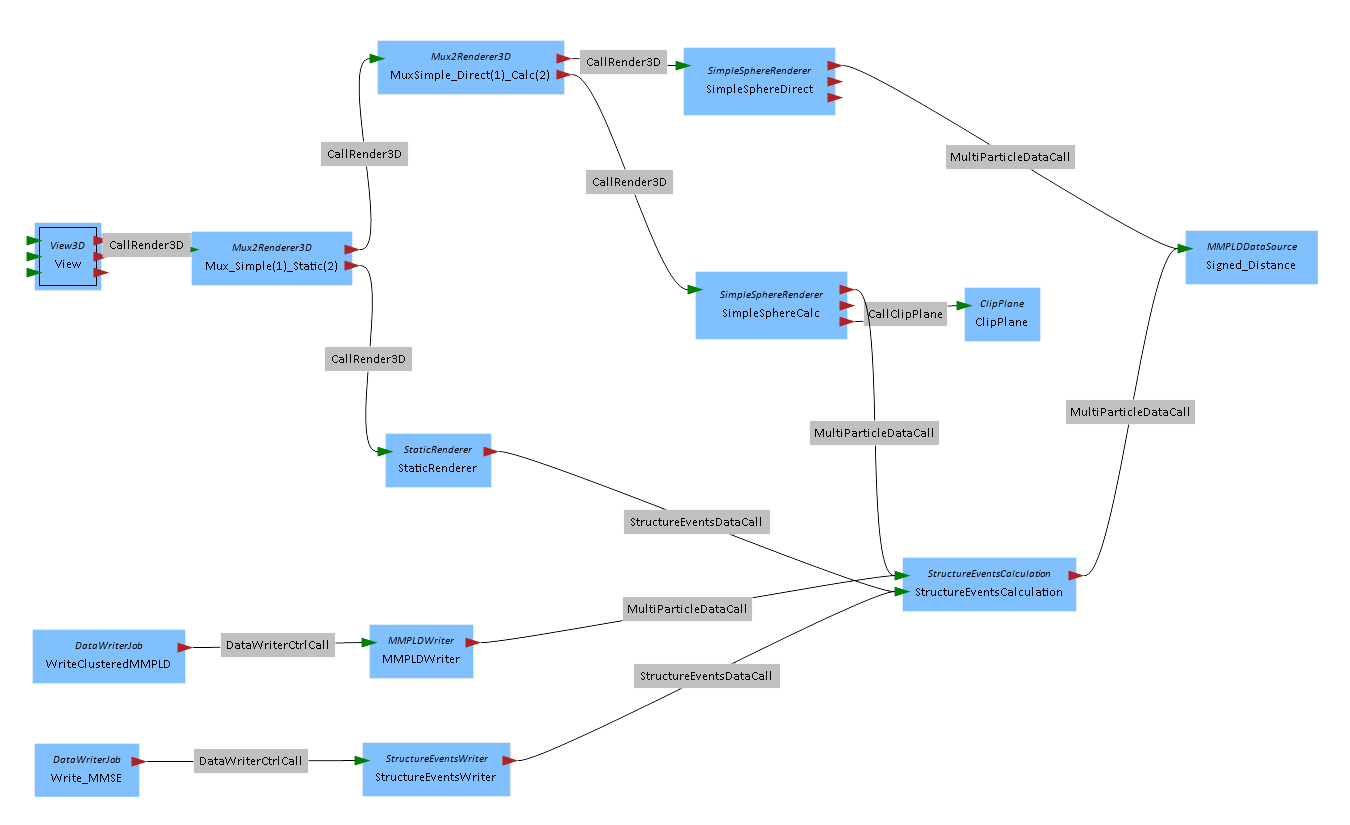
\includegraphics[width=1\textwidth]{pluginAufbau-writer}
	\caption{Anordnung der \tool{MegaMol} Module für die Überprüfung und Ausgabe der Berechnungen.}\label{fig:pluginAufbau-writer}
\end{figure}

Wie in \autoref{fig:pluginAufbau-writer} zu sehen, erfolgt die Speicherung der Clustervisualisierung in einem \gls{mmpld}, wozu das \MMStruktur{MMPLDWriter Modul} mit dem zugehörigen Job zum Einsatz kommt. Die Speicherung der Strukturereignisse geschieht durch das \MMStruktur{StructureEventsWriter Modul} bzw. innerhalb des \SECalc aufgrund spezieller Anforderungen des \tool{MegaMol} Jobsystems. Um eine schnelle visuelle Überprüfung der Ergebnisse vornehmen zu können, werden mehrere \MMStruktur{SimpleSphereRenderer} für die Partikel sowie die Ereignisvisualisierung mittels des \MMStrukturs{StaticRenderer Moduls}{StaticRenderer Modul} im selben Raum angezeigt. Dies ist durch die mehrfache Verschaltung des \MMStrukturs{MuxRenderers}{MuxRenderer} möglich.

Verbunden sind die Daten-, Berechnungs- und Visualisierungsmodule über den \SEDC bzw. des \gls{mpdc}. Wie der \gls{mpdc} sind die weiteren Module und Kommunikationsklassen Teil des \tool{MegaMol} Kerns. Das Viewmodul steuert unter anderem den angezeigten Frame. Die Auslösung der Berechnung für die unterschiedlichen Frames erfolgt durch den View über den verbundenen \MMStruktur{SimpleSphereRenderer}, da der aus \SECalc ausgehende \gls{mpdc} für den Wechsel der Frames verantwortlich ist.

Für die Berechnungen aller Frames wird Jobsystem von \tool{MegaMol} genutzt. Der Aufbau für die Jobs ist einfacher, da auf sämtliche Visualisierungsmodule verzichtet werden kann. Auch wird das \MMStruktur{StructureEventsWriter Modul} aufgrund von Restriktionen des Jobsystems in \SECalc integriert. Der Job wird auf dem \MMStruktur{MMPLDWriter Modul} aufgerufen, an dem das \SECalc mittels eines \gls{mpdc} angeschlossen ist, welches seine Daten durch einen weiteren, mit dem Lesemoduls für \gls{mmpld} Dateien verknüpften \gls{mpdc} bekommt. Dieses Modul liest den der Arbeit zugrundeliegenden Datensatz aus.

\subsection*{Programmaufbau für die Visualisierung}\label{sec:pluginaufbau-vis}
\begin{figure}
	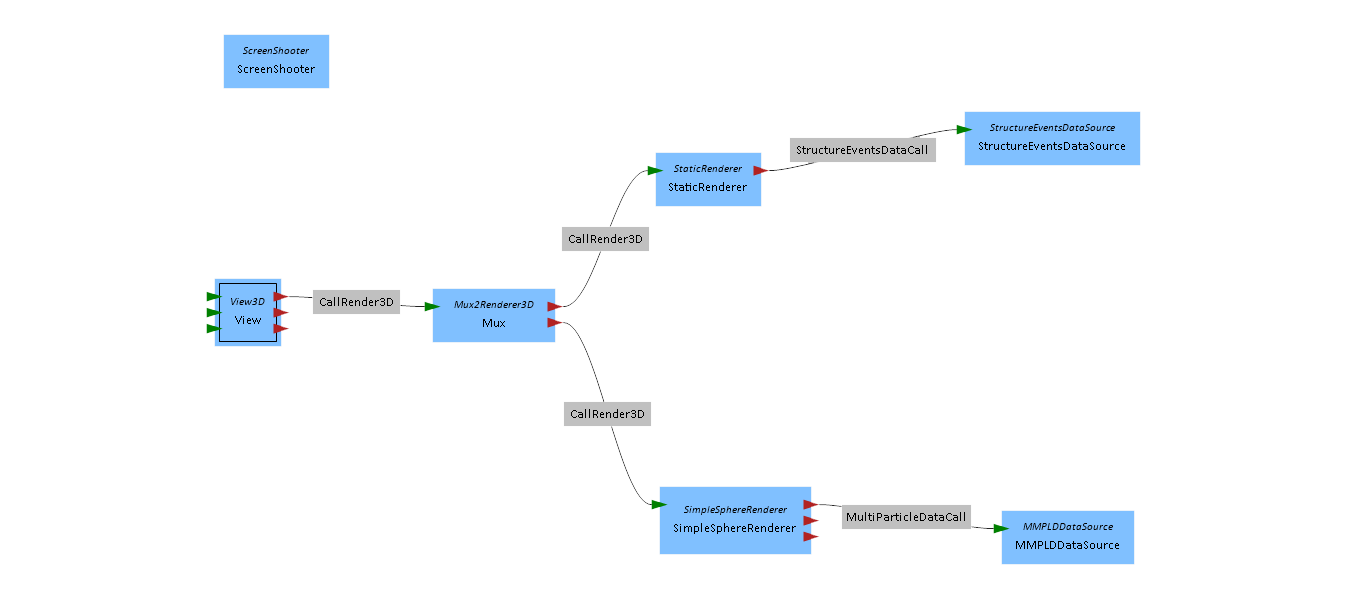
\includegraphics[width=1\textwidth]{pluginAufbau-reader}
	\caption{Anordnung der \tool{MegaMol} Module für die Ausgabe der erzeugten \gls{mmpld} und \MMSE Dateien.}\label{fig:pluginAufbau-reader}
\end{figure}

Die Ausgabe erfordert zwei Renderer. Den \MMStruktur{SimpleSphereRenderer} für die Visualisierung der Clustereinfärbungen und das \MMStruktur{StaticRenderer Modul} für die Strukturereignisse. Diese werden gemäß der geforderten, überlagerten Darstellung (siehe Superposition in \autoref{sec:related-visAnordnung}) mit Hilfe des \MMStrukturs{MuxRenderers}{MuxRenderer} im selben Simulationsraum angezeigt. Ihre Daten bekommen die Renderer jeweils von einem entsprechenden Lesemodul. 

Für die Ausgabe wurden Kernmodule modifiziert. Die wichtigste Modifikation ist die Ausblendung der in der Gasphase befindlichen Partikel mittels Deaktivierung von Partikeln mit der die Gasphase markierenden Farbe im entsprechenden Fragmentshader des \tool{MegaMol} Kerns. Diese Farbe ist in der aktuellen Implementation des Plugins über einen Slot in \SECalc festgelegt. Für eine langfristige Implementation dieses Features in \tool{MegaMol} müsste sie im \MMStruktur{SimpleSphereRenderer} durch den Nutzer einstellbar sein.

\begin{lstlisting}[language=c]
    // Discard fragments with certain color.
    if (gl_Color.r == .98 &&
	    gl_Color.g == .78 &&
	    gl_Color.b == 0.0)
	    discard;
\end{lstlisting}

\subsection*{Weiteres Optimierungspotential}\label{sec:pluginaufbau-optimierung}

\begin{itemize}
	\item \MMStruktur{SimpleSphereRenderer}: Filtern (Ausblenden) nach Partikelfarben wie oben vorgeschlagen
	\item \MMStruktur{StaticRenderer Modul}: Visuelle Ausgabe von quantitativen Ereigniswerten, analog zur Protokollierung in \SECalc.
	\item Globales Kennzeichen für die Logausgabe analog zum Protokollkennzeichen in \SECalc.
	\item WASD-QE-RF Steuerung, als Vorbild dienen die guten User Interfaces von Spielen wie Elite Dangerous
%	\item Hinzufügen eines Pfades für Texturen, indem zur megamol.cfg ein weiteres Element <texturedir> mit dem Attribut path hinzugefügt wird, analog zum Element <shaderdir>.
%	\item Hinzufügen eines Pfades für Logdateien zur Ausgabe von quantitativen Daten, indem zur megamol.cfg ein weiteres Element <outputFiledir> mit dem Attribut path hinzugefügt wird, analog zum Element <shaderdir>.
\end{itemize}


\section{Aufzählung der Cluster- und Ereigniserkennungsschritte}\label{sec:cluster-ereignis-schritte}

\begin{enumerate}
	\item
	\begin{enumerate}
		\item Aufbau der Partikelliste mit den Daten des \gls{mpdc}.
		\item Erstellung von kD-Bäumen für die Nachbarschaftserkennung
		\item Nutzung des kD-Baum Suchalgorithmus der \ANN, um Nachbarn jedes Partikels zu diesem hinzuzufügen unter Berücksichtigung des \CFDterm{Partikelradiusmultiplikator}
	\end{enumerate}
	\item
	\begin{enumerate}
		\item Cluster erstellen unter Nutzung der Nachbarn.
		\item Reduktion der \CFDterm{Mindestgrößencluster} innerhalb von Zusammenhangskomponenten, die weniger Partikel besitzen als für die benutzerdefinierte minimale \CFDterm{Clustergröße} erlaubt.
	\end{enumerate}
	\item \SECC durch Nutzung der \CFDterm{Clustervergleichsmatrix} und Erstellung von zwei Listen mit \SECterms{Partnerclustern}{Partnercluster} in vorwärtiger beziehungsweise rückwärtiger Richtung.
	\item Anwendung von Verhältnisberechnungen auf diese Listen und Nutzung von benutzerdefinierten Grenzwerten für die \SECterm{Ereignisheuristik}
\end{enumerate}

\section{Glyphprototyp}\label{sec:glyphprototyp}
Zur Überprüfung einer sinnvollen Zuweisung von Datenparametern zu den \viss{visuellen Variablen}{visuelle Variable} dienen Mockups. Aufgrund der Vielzahl der in \autoref{sec:strukturereignistaxonomie:zuweisung} genannten Kombinationsmöglichkeiten wird eine programmatische Erstellung der Mockups gewählt.

Dazu wird ein Glyphprototyp geschrieben, der \href{http://mmm.takera.de}{im Webbrowser verwendet werden kann}. Da eine schnelle Umsetzbarkeit im Vordergrund steht, wird \tool{Unity3D} als Entwicklungsumgebung gewählt. Ein Vorteil dieser Engine ist die Möglichkeit, rasch Prototypen erstellen zu können sowie die einfache Umsetzbarkeit für verschiedenste Plattformen, ohne auf Containermanager wie \href{https://www.docker.com/}{Docker} angewiesen zu sein.
%Letzterer Umstand ist für den möglichen Einsatz der Mockups als Evaluationswerkzeug von Bedeutung.
Die Geschwindigkeit der graphischen Anzeige spielt bei der Erstellung von Mockups eine untergeordnete Rolle.

%Beim Deploy der \tool{Unity3D} WebGL Anwendung kam es auf bestimmten Apachekonfigurationen zu Problemen. Dies war durch eine \href{http://forum.unity3d.com/threads/html-mem-causes-http-500-internal-server-error-on-apache.309762/}{manuelle Umbenennung von Dateien und Verweisen} in der durch \tool{Unity3D} generierten Anwendung zu lösen. Von offizieller Seite wurde dies \href{http://forum.unity3d.com/threads/html-mem-causes-http-500-internal-server-error-on-apache.309762/#post-2014787}{als Bug markiert}. SOLCHE SÄTZE HABEN IN DER BA VERMUTLICH NIX ZU SUCHEN?

Der Glyphprototyp basiert auf einer älteren Entwicklungsstufe der \vis{Strukturereignistaxonomie}, in der die Opazität vorhanden war und die Textur fehlte. Dies wirkt sich nicht nachteilig aus. Zum Einen erfolgt im Prototyp keine überlagerte Darstellung mit einem anderen Datenobjekt. Zum Anderen wird er in dieser Arbeit nur zur Überprüfung der dreidimensionalen Glyphdarstellung genutzt. Der Vorteil in der Verwendung der Opazität liegt darin, dass so das in \autoref{sec:glyphprototyp:opazitaet} beschriebene, günstige Verhalten der Opazität bei der Zuweisung zur Häufung genutzt werden kann.

\subsection*{Erstellung des Datensatzes}\label{sec:glyphprototyp:daten}
Um eine Vergleichbarkeit der verschiedenen Mockups zu gewährleisten, liegt ein fester Datensatz zugrunde. Sämtliche Werte wurden für die Datenparameter Ort und Zeit so gewählt, dass eine Überlappung der Ereigniselemente von nebeneinanderliegenden Ereignissen bei einer Zuweisung an die \vis{visuelle Variable} Position nicht auftritt, da andernfalls durch das \vis{Gesetz der verbundenen Elemente} ein falsches Abbild der zugrundeliegenden Daten übertragen werden würde. Der Zahlenbereich für die Zeit ist auf das Intervall $[1,22]$ begrenzt. Da sich in der Simulation die meisten Elemente mit zunehmender Zeit vom Zentrum entfernen, wird die $x$-Koordinate des Ortes mit \autoref{eq:glyphprototyp:zeit-ortx} direkt an die Zeit $t$ gekoppelt.
\begin{align}\label{eq:glyphprototyp:zeit-ortx}
	x = \left\lfloor\frac 43\cdot t + 0,5\right\rfloor
\end{align}
Aufgrund des zylinderförmigen Raumes in der Simulation wird sowohl für die $y$-Koordinate als auch für die $z$-Koordinate des Ortes ein identisches und kleineres Intervall von $[1,10]$ gewählt.

Die Zuweisung der Ereignisart erfolgt manuell. Da die Partikel des \gls{mmpld} Quelldatensatzes zu Beginn der Simulation einen einzigen Cluster in flüssiger Phase bilden (siehe \autoref{sec:simulation}), werden im Prototypen bei kleinen Zeitwerten vornehmlich Splits zugewiesen.

Zur Darstellung der in \autoref{sec:strukturereignistaxonomie:haeufung} beschriebenen Häufung, %werden die Ereignisse $6-9$, $35/36$ sowie $46-48$
werden einige Ereignisse jeweils gruppiert und händisch an denselben Ort und dieselbe Zeit gesetzt. Weiterhin wird, wie in \autoref{sec:strukturereignistaxonomie:haeufung} empfohlen, die Häufung als Ereignisparameter implementiert, um ihr visuelle Variablen zuweisen zu können.

\subsubsection*{Zuweisung der Zahlenwerte}
Zur Gewährleistung der in \autoref{sec:glyphprototyp:daten} beschriebenen Vermeidung unnötiger Überlappungen der Ereigniselemente wird der Standardwert der \viss{visuellen Variable}{visuelle Variable} Größe, d.h. wenn die Variable keinem Parameter zugewiesen ist, entsprechend skaliert. Um nah bei der Visualisierung der Molekularsimulation selbst zu bleiben, wird in den Mockups, die die \vis{visuelle Variable} Form nicht beinhalten, eine Kugel verwendet. 

Die Variablen in den Mockups weisen folgende Zahlenbereiche auf:
\begin{itemize}
	\item x-, y-, z-Position: $[-\infty, \infty]$, beim Parameter Ort erfolgt eine direkte Zuweisung 
	\item Farbwert: $[0, 340]\degree$ bei $100\%$ Sättigung (\gls{hsb} Modell)
	\item Helligkeit $[40, 100]\%$, Standardwert $100\%$ (\gls{hsb}-Modell)
	\item Form: besitzt keinen Zahlenbereich, sondern beinhaltet verschiedene Formen von Polyedern sowie die Kugel als Standardwert
	\item Skalierung: $[0.25,2]$, Standardwert $1$
	\item Opazität: $[40, 100]\%$, Standardwert $100\%$
\end{itemize}
Die Mindesthelligkeit $b_{\text{min}}$ von $40\%$ dient dazu, um noch eine Farbwertunterscheidung treffen zu können, genauso wie die Mindestopazität von ebenfalls $40\%$. Der Maximalfarbwert $h_{\text{max}}$ von $340\degree$ wird festgelegt, um eine Unterscheidung zu den niedrigen Farbwerten zu erhalten.

Da die Grenzwerte der \viss{visuellen Variablen}{visuelle Variable} $a_{\text{min}}$ und $a_{\text{max}}$ bekannt sind und sich für die Parameter $p$ des Datensatzes ein minimaler und maximaler Wert $p_{\text{min}}$ und $p_{\text{max}}$ bestimmen lässt, wird für die Berechnung der Variablenwerte die Linearfunktion in \autoref{eq:glyphprototyp-linearfunktion} verwendet.

\begin{equation}
\begin{aligned}\label{eq:glyphprototyp-linearfunktion}
a &= m \cdot p + n\\
a_{\text{max}} &= m \cdot p_{\text{max}} + n\\
a_{\text{min}} &= m \cdot p_{\text{min}} + n\\
m &= \boxed{\frac{a_{\text{max}} - n}{p_{\text{max}}}}\\
n &= a_{\text{min}} - m \cdot {p_{\text{min}}} = a_{\text{min}} - \frac{a_{\text{max}} - n}{p_{\text{max}}} \cdot p_{\text{min}}\\
&= a_{\text{min}} - a_{\text{max}} \cdot \frac {p_{\text{min}}}{p_{\text{max}}} + n \cdot \frac {p_{\text{min}}}{p_{\text{max}}}\\
n \cdot p_{\text{max}} &= a_{\text{min}} \cdot p_{\text{max}} - a_{\text{max}} \cdot p_{\text{min}} + n \cdot p_{\text{min}}\\
n \cdot \left( p_{\text{max}} - p_{\text{min}}\right) &= a_{\text{min}} \cdot p_{\text{max}} - a_{\text{max}} \cdot p_{\text{min}}\\
n &= \boxed{\frac{a_{\text{min}} \cdot p_{\text{max}} - a_{\text{max}} \cdot p_{\text{min}}}{p_{\text{max}} - p_{\text{min}}}}\\
\end{aligned}
\end{equation}

Anschließend erfolgt eine Rundung zur handlichen Verwendung der Ergebnisse.
\begin{align}\label{eq:glyphprototyp-rundung}
	a = \left\lfloor m \cdot p + n + 0,5 \right\rfloor
\end{align}

Aufgrund des großen Umfangs und der geringen Relevanz der Berechnungsergebnisse sind sie hier nicht aufgeführt.
%Die Berechnungsergebnisse sind in \autoref{sec:mockups:berechnungen} zu finden.

\subsubsection*{Zuweisung des Vokabulars}

Da die Mächtigkeit $M$ des Vokabulars der Ereignisart bekannt ist, kann das Intervall $v$ der \viss{visuellen Variable}{visuelle Variable} $a$ in \autoref{eq:glyphprototyp-vokabular} zur rechnerischen Ermittlung der Variablenwerte $a_i$ genutzt werden.

\begin{equation}
\begin{aligned}\label{eq:glyphprototyp-vokabular}
M &= 4\\
\Rightarrow p_{0\ldots 3} &= \left( 0, \frac 13, \frac 23, 1 \right) \\
v &= a_{\text{max}} - a_{\text{min}}\\
\\
a_i &= \left\lbrace p_i \cdot v + a_{\text{min}} \left| 0 \le i \le M-1 \right. \right\rbrace 
\end{aligned}
\end{equation}

Ausnahmen bilden die \viss{visuellen Variablen}{visuelle Variable} Farbe und Form. Wegen der kleinen Mächtigkeit des Vokabulars und zur Sicherung einer optimale Aufteilung des Farbwerts, wird dieser in \autoref{tab:glyphprototyp:ereignisart} manuell definiert. Für die Form werden zur optimalen Unterscheidung vier Varianten aus der Menge der \viss{platonischen Körper}{platonischer Körper} ausgewählt.

\begin{table}
	\begin{tabularx}{\textwidth}{@{}CRRRCR@{}}
		\toprule
		Art & Farbwert [°] & Helligkeit [\%] & Position x & Form & Größe \tabularnewline
		\midrule
		Birth & 145 & 100 & 31 & D & 2 \tabularnewline
		Death & 0   & 40  & 1  & T & 0,25 \tabularnewline
		Merge & 55  & 60  & 11 & H & 0,83 \tabularnewline
		Split & 245 & 80  & 21 & O & 1,42 \tabularnewline
		\bottomrule
	\end{tabularx}
	\caption{Festlegung der Attributeigenschaften für die Ereignisart in den Mockups.}\label{tab:glyphprototyp:ereignisart}
\end{table}

\subsubsection*{Konstanter Variablenwert bei Opazität}\label{sec:glyphprototyp:opazitaet}
Die Reservierung der Opazität für die Häufung ist sinnvoll, denn dies hat zwei Vorteile. Zum Einen ist keine nachträgliche Modifizierung der visuellen Attribute der einzelnen Ereignisse notwendig, denn die Opazitätseigenschaft sorgt durch Überlagerung für eine von der Anzahl direkt abhängige Hintergrundverdeckung. Dadurch werden zum Anderen auch keine Informationen über die Häufigkeit im Datensatz benötigt. Hingegen wird zum Beispiel bei der Zuweisung des visuellen Attributes Größe eine Größenveränderung nachträglich für jedes Ereignis in der Anhäufung auf der Basis eines temporalen oder lokalen Häufungswertes durchgeführt.

Aufgrund dieses günstigen Verhaltens der Opazität wird ihr ein konstanter Variablenwert zugewiesen, so dass keine zusätzlichen Ereigniswerte für die Häufung benötigt werden. Dieser konstante Wert wird auf $50\%$ Opazität festgesetzt.

\subsection*{Unterscheidbarkeit von Polyedern}\label{sec:polyeder}
Da die Unterscheidung von Polyedern mit zunehmender Flächenanzahl schwieriger wird, findet im Glyphprototyp eine Begrenzung auf die fünf \viss{platonischen Körper}{platonischer Körper} mit einer geringen Ecken- und Flächenanzahl statt.
\begin{description}
	\item[T] Tetraeder mit 4 Ecken und 4 Flächen
	\item[O] Oktaeder mit 6 Ecken und 8 Flächen
	\item[H] Hexaeder mit 8 Ecken und 6 Flächen
	\item[I] Icosaeder mit 12 Ecken und 20 Flächen
	\item[D] Dodekaeder mit 20 Ecken und 12 Flächen
\end{description}
Die Abkürzungen folgen dem Vorschlag von Baierl \cite[S.~42]{KonvexePolyeder}. Bei der Modellierung in \tool{Blender} wurde für die Polygonnetze die maximale Dimension von $1$ (einheitenlos) entsprechend der Dimension der kugelförmigen Standardelemente in \tool{Unity3D} gewählt.


\section{Berechnungen Glyph}\label{sec:berechnungen:glyph}
Die folgenden Berechnungen sind abhängig von der Ereigniszeit $t$ mit $t_{\text{max}}$ als höchsten Zeitpunkt aller Ereignisse. Die Farben werden im \gls{hsv}-Farbraum berechnet.

Berechnung des Farbwertes $h$ im Intervall $[0,1]$ mit $h_{\text{offset}} = \frac{30\degree}{360\degree}$ als Versatz zur Vermeidung identischer Farbwerte am Anfang und Ende des Zeitraums. Die Sättigung $s$ und Helligkeit $v$ sind maximal $s = v = 1$.
\begin{equation}
\begin{aligned}\label{eq:berechnungen:glyph-farbe}
h &= \left(\frac{t}{t_{\text{max}}}\right) \cdot (1 - h_{\text{offset}}) + h_{\text{offset}}
\end{aligned}
\end{equation}

Berechnung der Helligkeit $v$ im Intervall $[0,1]$ mit $b_{\text{offset}} = 0,4$ als Versatz zur Vermeidung identischer Helligkeitswerte am Anfang und Ende des Zeitraums. Der Farbwert ist ein Blauton $h = \frac{208\degree}{360\degree}$ und die Helligkeit $v$ ist maximal $v = 1$.
\begin{equation}
\begin{aligned}\label{eq:berechnungen:glyph-helligkeit}
v &= \left(\frac{t}{t_{\text{max}}}\right) \cdot (1 - b_{\text{offset}}) + b_{\text{offset}}
\end{aligned}
\end{equation}

Berechnung der Höhe der dunkelgrauen Texturfarbe $p$ im Intervall $[0,1]$ mit $p_{\text{offset}} = 0,01$ als Versatz zur Korrektur des unteren Transparenzbereiches der Textur. %Die Farbe ist weiß $hsv = (0, 0, 1)$.
\begin{equation}
\begin{aligned}\label{eq:berechnungen:glyph-textur}
p &= \left(\frac{t}{t_{\text{max}}}\right) \cdot (1 - p_{\text{offset}}) + p_{\text{offset}}
\end{aligned}
\end{equation}

\section{Verwendete Hardware}\label{sec:hardware}
Das Plugin wurde auf folgendem System entwickelt:
\begin{itemize}
	\item Prozessor: Intel Core i5-3210M @2,5GHz
	\item Arbeitsspeicher: 2x4 \gls{GiB} DDR3-1600
	\item Betriebssystem: Windows 8.1
\end{itemize}
Wenn nicht anders gekennzeichnet, beziehen sich die Zeit- und Ressourcenangaben auf dieses System.

Die Berechnung aller Frames wurden aufgrund des hohen Ressourcenverbrauchs auf folgendem System durchgeführt
\begin{itemize}
	\item Prozessor: Intel Core i5-3570K @3,4GHz
	\item Arbeitsspeicher: 2x8 \gls{GiB} DDR3-1600
	\item Betriebssystem: Windows 8.1
\end{itemize}

\section{Werkzeuge und Bibliotheken}\label{sec:werkzeuge}

\subsubsection{Mockup Visualisierung}
\begin{description}
	\item [Adobe Illustrator]
	\item [Blender] mit Regular Solids
	\item [Unity3D] mit \href{http://forum.unity3d.com/threads/a-working-stylable-combo-box-drop-down-list.264167/}{UIComboBox}, \href{http://forum.unity3d.com/threads/fly-cam-simple-cam-script.67042/}{Simple FlyCamera} 
\end{description}

\subsubsection{Dokumentation}
\begin{description}
	\item [Adobe Photoshop]
	\item [Blender] mit Extra Objects
	\item [Fraps] Aufnahme der visuellen MegaMol Ausgaben
	\item [IrfanView] Bildumwandlung
	\item [TeXstudio, TeXlive] mit tudscr, glossaries, tikz u.a.
\end{description}

\subsubsection{MegaMol Plugin}
\begin{description}
	\item [ActivePerl]
	\item [Adobe Illustrator] zur Gestaltung der Glyphen
	\item [Adobe Photoshop] zur Erstellung der Texturen
	\item [glm] zur Speicherung von Vektoren analog zu \tool{OpenGL}.
	\item [lodepng] zum Laden von Texturen
	\item [MegaMol] mit \ANN, AntTweakBar, mmstd\_datatools, vislib
	\item [MegaMolConf]
	\item [VisualStudio 2013] mit \href{http://openmp.org/}{OpenMP} und \href{https://msdn.microsoft.com/en-us/library/dd492418.aspx}{Parallel Patterns Library}
\end{description}

\subsubsection{Konturbäume}
In der Implementation nicht genutzt, aber aufgrund des Schwerpunktes in der Analyse mit aufgeführt.
\begin{description}
	\item [SimpleCT]  \href{https://github.com/baranaydogan/SimpleCT/}{Repository} \cite{aydogan2013contourTreeBinary}
	\item [libtourtre] \href{http://graphics.cs.ucdavis.edu/~sdillard/libtourtre/doc/html/}{Website}, basierend auf \cite{carr2001computingCountourTrees} und \cite{pascucci2004multiResolutionComputation}
\end{description}

\section{Alternative Bestimmung der Cluster ohne Nachbarschaftskenntnisse}\label{sec:cluster-radial}
Partikel eines Clusters können über eine radialbasierte Nachbarschaftsbeziehung bestimmt werden, wobei vom Partikel mit der größten Tiefe, dem sogenannten \contour{Saatpartikel} begonnen wird.

Um diesen Prozess zu beschleunigen, werden beim Auslesen der MMPLD Daten alle Partikel nach ihrem \contour{Tiefenwert} in einer Liste sortiert, analog zum ersten Schritt des Abtastalgorithmus (siehe \autoref{sec:related:konturAbtast}). Eine speichersplatzsparendere Methode, die auf das Kopieren aller Partikel im Speicher verzichtet, wäre das Nutzen von Zeigern auf den vorhandenen Datensatz, allerdings wäre zum Einen eine Änderung der Daten aufwändig (Lockingmechanismen) und der nächste \contour{Tiefenwert} müsste bei jeder Partikelbehandlung aus dem ursprünglichen MPDC erneut herausgesucht werden.

Ausgehend vom \contour{Saatpartikel} werden die Partikel in der Liste abgelaufen und in eine neue Liste gespeichert. Sollte der nächste Partikel, der den gleichen oder einen etwas geringeren \contour{Tiefenwert} aufweist, in einem bestimmten Radius zum vorhergehenden Partikel liegen, so wird dieser in dieselbe Liste geschrieben, ansonsten in eine andere. Der Radius, mit dem geprüft wird, hängt von der Differenz des \contours{Tiefenwertes}{Tiefenwert} zwischen betrachteten Partikel und Minimalpartikel der aktuellen Liste ab. Sollte der Partikel außerhalb dieses Radius' liegen, wird eine neue Liste erstellt. Eine Ausnahme bilden Partikel mit negativem \contour{Tiefenwert}. Sie werden in eine separate Liste geschrieben und es erfolgt keine Positionsprüfung. Jede Liste enthält einen Offset. Dort befindet sich der Listenidentifikator.

Dieser Algorithmus ist wegen der Entfernungsbestimmung über den Radius sehr langsam. Zur Beschleunigung könnte die Entfernungsbestimmung bei den Partikeln auf solche mit ähnlichen Tiefenwerten eingeschränkt werden %$O(n^2 - k | k = n_{SignedDistance} > intervall)$
oder es könnte eine Einteilung des Raumes in ein Gitter erfolgen und jede Zelle erhält ihre eigene Partikelliste. Bei der Suche nach benachbarten Partikeln werden nur die Nachbarzellen durchsucht. Allerdings ist auch bei diesen Varianten immer noch eine Entfernungsbestimmung notwendig, wenn auch mit wesentlich weniger Überprüfungen je Partikel.

Daher werden diese Methoden nicht weiter verfolgt und stattdessen wird auf eine Baumstruktur zur Nachbarschaftsbildung zurückgegriffen und von diesen Daten aus eine Clusterbestimmung vorgenommen (siehe \autoref{sec:nachbarschaftssuche}).

%\backmatter %Nachspann: Römische Seitennummerierung

\printbibliography[heading=bibintoc]\label{sec:bibliography}

\printindex % Überschriftentyp in \indexsetup, level

\end{document}